\documentclass{article}
\usepackage{float}
\usepackage{graphicx}
\usepackage{subfig}
\usepackage{lipsum}
\usepackage{tikz}
\usepackage{eso-pic}
\usepackage{changepage}
\usepackage{xcolor}
\usepackage{afterpage}
\usepackage[document]{ragged2e}
\usepackage[none]{hyphenat}
\usepackage[margin=1in,footskip=0.25in]{geometry}
\usepackage{array}
% \usepackage{l3kernel}
% \usepackage{l3packages}
\usepackage{siunitx}
\usepackage{color,soul}
\usepackage{placeins}
\usepackage{microtype}
\usepackage[backend=biber]{biblatex}
\usepackage[hidelinks]{hyperref}
\usepackage[toc,page]{appendix}
%\usepackage[toc]{glossaries}
\usepackage[subfigure]{tocloft}
\usepackage{rotating}
\usepackage[printwatermark]{xwatermark}
% \usepackage[table,xcdraw]{xcolor}
\usepackage{xcolor}
\hypersetup{
	colorlinks,
	linkcolor={black!50!black},
	citecolor={blue!50!black},
	urlcolor={blue!80!black}
}

\cftsetindents{subsection}{.25in}{.4in}

\usepackage[flushleft]{threeparttable}
\newcolumntype{C}[1]{>{\centering\let\newline\\\arraybackslash\hspace{0pt}}m{#1}}

\definecolor{ULred}{HTML}{872434}

\usepackage{chngcntr}
\counterwithin{table}{section}
\counterwithin{figure}{section}

\pdfoptionpdfminorversion=6
%\addbibresource{FireAttackReport.bib}

\setlength{\parskip}{1em}

% ******* REMOVE COMMENTS AND PLACE GLOSSARY.TEX IN ROOT DIRECTORY TO ADD GLOSSARY, SEE END FOR ADDITIONAL LINES TO UNCOMMENTS *******
%
%\loadglsentries{glossary.tex}
%
%\makeglossaries

% ******* REMOVE COMMENTS ON THIS BLOCK TO ADD DRAFT TO REPORT ********
% \newsavebox\mybox
% \savebox\mybox{\tikz[color=gray,opacity=0.5]\node{DRAFT};}
% \newwatermark*[
% allpages,
% angle=65,
% scale=15,
% xpos=-65,
% ypos=20
% ]{\usebox\mybox}

\begin{document}
	
	\begin{titlepage}
		
		\pagecolor{ULred}\afterpage{\nopagecolor}
		

		\AddToShipoutPictureFG*{\AtPageUpperLeft{\raisebox{-\height}{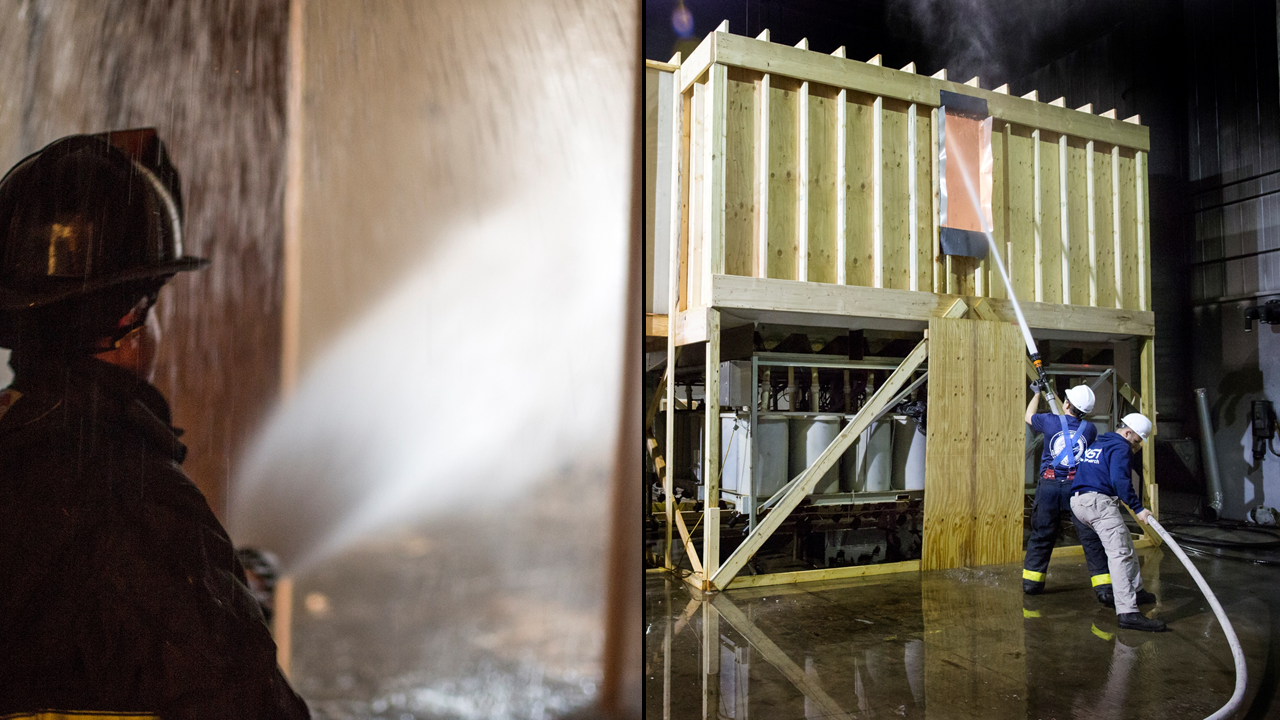
\includegraphics[width=7in]{Figures/General/TitlePagePhoto.png}}}} 

			\vspace*{20\baselineskip} 

		\huge
		\begin{adjustwidth}{-0.5in}{-0in}
		\color{white}
		\textbf{Study of the Impact of Fire Attack \\ Utilizing Interior and Exterior Streams \\ on Firefighter Safety and Occupant Survival}
		\end{adjustwidth}
		\huge
		\begin{adjustwidth}{-0.5in}{-0in}
		\color{white}
		\textbf{Part I: Air Entrainment and Water Distribution}
		\end{adjustwidth}
		\begin{adjustwidth}{-0.5in}{}
		\color{white}
		\vspace{.2\baselineskip}
		\large
		Stephen Kerber \\
		Director \\
		UL Firefighter Safety Research Institute \\
		\vspace*{.5\baselineskip}
		Robin Zevotek \\
		Lead Engineer \\
		UL Firefighter Safety Research Institute \\ 
		\vspace*{.5\baselineskip}
		Keith Stakes \\
		Research Engineer \\
		UL Firefighter Safety Research Institute \\
		\vspace*{.8\baselineskip}	
		\today
		\vspace*{.8\baselineskip}
		\begin{figure}[h]
			\hspace*{-0.5in}
\includegraphics[width=0.75in]{../0_Images/ULLogoWhite.pdf}
		\end{figure}
		\end{adjustwidth}
	\end{titlepage}

\begin{center}
	DISCLAIMER\\
	\vspace*{\baselineskip}
	\begin{adjustwidth}{-0.25in}{-0.25in}
		In no event shall UL be responsible to anyone for whatever use or non-use is made of the information contained in this Report and in no event shall UL, its employees, or its agents incur any obligation or liability for damages including, but not limited to, consequential damage arising out of or in connection  with the use or inability to use the information contained in this Report. Information conveyed by this Report applies only to the specimens actually involved in these tests. UL has not established a factory Follow-Up Service Program to determine the conformance of subsequently produced material, nor has any provision been made to apply any registered mark of UL to such material. The issuance of this Report in no way implies Listing, Classification or Recognition by UL and does not authorize the use of UL Listing, Classification or Recognition Marks or other reference to UL on or in connection with the product or system.
	\end{adjustwidth}
\end{center}

\begin{center}
	FUNDING
\vspace*{\baselineskip}
\begin{adjustwidth}{-0.25in}{-0.25in}
This work was funded through a grant from the Department of Homeland Securities Assistance to Firefighters Grant Program under the Fire Prevention and Safety Grants, Research and Development.
\end{adjustwidth}
\end{center}

\begin{center}
	
\includegraphics[width=0.28\textwidth]{Figures/General/DHS.png}
\end{center}

\clearpage

\renewcommand{\abstractname}{Abstract}
\setlength{\emergencystretch}{5pt}

\begin{abstract}

As research continues into how fire department interventions affect fire dyanmics in the modern fire environment; questions continue to arise on the impact and implications of interior versus exterior fire attack on both firefighter safety and occupant survivability. Previous research into various types of fire ground ventilation, flow paths, and exterior fire streams has provided the fire service with a more in-depth understanding of fire dynamics in addition to raising questions about certain fire attack methods stemming from differing traditions and myths. This knowledge gap and lack of previous research into the impact of fire streams has driven the need for further research into fire department interventions at structure fires with a focus on hose streams and suppression tactics. Statistics show that both firefighters and building occupants continue to loose their lives due to fire. As such, research into the various methods of fire attack will allow a broader understanding of how firefighter interventions on the fire ground can impact the outcome of both life safety and property protection. 

This study will build and expand upon the fire research conducted to date by analyzing how firefighting tactics, specifically suppression methods, affect the thermal exposure and survivability of both firefighters and buidling occupants in addition to impacting fire behavior in structures. The project will be comrprised of 3 parts:
\vspace*{\baselineskip}
\begin{itemize}
	\item Part I: Air Entrainment and Water Distribution.
	\item Part II: Full-scale Residential Fire Experiments.
	\item Part III: Acquired Structure Fire Testing.
	\end{itemize}
\vspace*{\baselineskip}
This report details the experimental data from the air entrainment and water distribution experiments. Results from the first two experiment series were analyzed and reviewed with assistance from our technical panel. These results were summarized into tactical considerations and can be seen below:

\vspace*{\baselineskip}
\noindent \bf{Air Entrainment} -
\normalfont
\begin{itemize}
	\item Air entrainment in nozzles is dependent on nozzle type (smooth bore, straight stream, fog) and not nozzle manufacturer.
	\item Air entrainment in nozzles is dependent on structure geometry and configurations.
	\item Nozzle application patterns have little effect on overall air entrainment.
	\item Air entrainment, either into or out of the structure, is dependent on the distance of the nozzle to the ventilation opening.
	\end{itemize}
\vspace*{\baselineskip}
\noindent \bf{Water Distribution} -
\normalfont
\begin{itemize}
	\item Water distribution is dependent on nozzle type (smooth bore, straight stream, fog).
	\item Water distrubtion is dependent on stream direction within a compartment (max angle, mid ceiling, min angle).
	\item Varying nozzle pressure and flow can affect the amount of water applied to a given area while the distribution remains somewhat constant.
	\item Applying water from the exterior or from a distance via the interior will adequately coat the surfaces of a compartment (walls and ceiling) while applying little water to the center of the room.
	\end{itemize}
\vspace*{\baselineskip}

\end{abstract}

\newpage

\tableofcontents

\newpage

\section*{Introduction}

The purpose of this study is to improve firefighter safety, fireground tactics, and the knowledge of fire dynamics by providing the fire service with credible scientific information, developed from both water flow and full-scale fire testing, in representative single family homes, on the impacts and implications of both interior and exterior fire attack. Part I of the study is aimed at quantifying air entrainment in nozzles to provide insight into how hose streams move air inside buildings and determining where water is distributed in compartments. These series of tests were conducted without the presence of fire in order to gain a basic understanding of air flow and water flow before Parts II and III of the study were conducted as full-scale fire experiments. The full-scale fire experiments were designed based on the results from Part I of this study. Each test in Part I was designed to evaluate the differences in air entrainment and water distribution by testing various application methods, nozzle types and patterns, pressures/flows, and stream location and angles. Over 150 tests were performed for air entrainment and more than 80 tests were performed for water distribution. 

\clearpage

\section{Background}

Recent fire service research has highlighted the importance of applying water to the fire as quickly as possible. This tactical consideration has highlighted a knowledge gap and increased the interest in better understanding the impact of water applied as part of an interior attack or exterior attack. Many variables exist in fire attack that impact firefighter effectiveness and victim survivability, stream placement, the timing required to get water on the fire, stream type, stream movement, air entrainment, steam development, hot gas cooling and contraction and position of flow paths. The fire service's most important tool for many years at structure fires is their hose line, however many questions have arisen as more research shows the impact of ventilation, flow paths and exterior fire streams. Whether a fire attack crew chooses to apply water as part of an interior attack or as part of an exterior or transitional attack they need to know what impact their stream has on the fire environment ahead of them. This is difficult on the fire ground because visibility is commonly limited and therefore all of their experience is from behind the nozzle. This results in beliefs about conditions (e.g., temperature), ahead of the nozzle and its impact on victim survivability but knowledge of actual impact has not been researched. Additionally, when the fire is ultimately suppressed that does not mean it was done most effectively, efficiently and safely but the experience gained suggests that it was. Fire service adages such as ``don’t put water on smoke,'' ``you will steam the victims,'' and ``fog nozzles always disrupt the thermal layer'' have been passed on from generation to generation with little context or substantiation. Without the context these concepts get treated like rules and can severely limit firefighters understanding of fire suppression.

Fire training curriculum defines 3 fire attack methods, direct attack, indirect attack and combination attack. Direct attack involves the discharge of water directly onto the burning fuel. Indirect attack involves directing the stream toward the ceiling of a compartment in order to generate a large amount of steam in order to cool the compartment. Converting the water to steam displaces oxygen, absorbs the heat of the fire and cools the hot gas layer sufficiently for firefighters to safely enter and make a direct attack. Combination attack extinguishes a fire by using both a direct and indirect attack. Another technique to safely approach a fire that cannot be reached with a direct attack is gas cooling. Gas cooling provides a buffer zone around the attack team but the larger the compartment the less the impact on cooling the hot gas layer. Gas cooling must be a continuous process while advancing toward a shielded fire. Techniques for effective gas cooling and the upper limit of the volume where gas cooling is effective is not well known.  

In fire fighter training there is a lot of emphasis on steam generation but little is taught or demonstrated about the mechanics of suppression. Water vaporized in the upper gas layer reduces the total volume of the hot gases and steam. Water vaporized on hot surfaces such as the ceiling does not take much energy from the fire and therefore the volume of steam produced lowers the upper layer and makes conditions less tenable. These concepts are very important when the fire is not able to be directly attacked by applying water on burning fuel but is very difficult to visualize during a fire attack with limited visibility. Many of these fire suppression concepts are difficult to learn and refine because realistic ventilation limited fires are not safely replicated in firefighter training structures. Conditions created by todays fuels with heat release rates and smoke production properties commonly found in our structures are not allowed when following fire service training standards. Therefore the impact of hose streams in concrete training structures or metal containers can be misleading to firefighters resulting in incorrect inferences. This may then lead to inappropriate fire ground tactics with potentially deadly results. Research is needed to better understand the impact of hose streams so that proper messages can be taught in fire service training programs.

There are potentially harmful effects of inappropriate water application regardless of the type of hose stream. Since firefighters today are more aware of the need to cool hot smoke (fuel) in the upper layer, it is essential to understand the capabilities and limitations of each type of stream. The impact of hose stream application as one advances during a fire attack is dependent on a number of factors, principle of which are the flow path and where the steam is produced (in the hot gas layer or on contact with hot surfaces). Continuous application is likely to result in more steam being produced than gas contraction in the hot gas layer. Without ventilation in front of the hose stream, this can result in a reduction in tenability. However, when victims or firefighters are not in the flow path, and ventilation is in front of the hose stream, a combination attack can be quite effective for fully developed fire conditions.

Fire suppression effectiveness and firefighter safety are not achieved by water flow rate alone, but by appropriate use of a given flow rate under specific fire ground conditions. A flow rate must meet the critical flow rate to extinguish a fire depending on the heat release rate and should be higher to reduce the time to extinguishment. Drastically exceeding the critical flow rate has less impact on time to extinguishment but has a significant impact on the total amount of water used. There is little data to support that dramatically exceeding the critical flow rate results in increased firefighter safety. It has been estimated that only 5 to 10 percent of water applied during fire attack contributes to extinguishment. It is difficult for firefighters to realize the the efficiency of various hose stream techniques due to poor visibility on the fireground. However, by developing data in realistic structures, fuel sources, and fire scenarios, important inferences may be developed relative to different hose stream techniques, and use of water.

\clearpage

\section{Objectives and Technical Plan}

\subsection {Objectives}

The purpose of this study was to provide the fire service with scientific based knowledge on the impact of interior and exterior fire attack tactics on firefighter safety and trapped occupants to improve training and decision making on the fire ground. This was accomplished with the completion of the following objectives:

\begin{itemize}
	\item Improve firefighter safety by increasing knowledge of fire behavior.
	\item Develop knowledge of water streams applied during an interior and exterior/interior fire attack and its impact on firefighter safety and victim survivability.
	\item Understand where water goes and how air flows during interior and exterior/interior fire attack utilizing common procedures and what that means to fire dynamics within a structure.
	\item Gain understanding of the impact of water streams depending on the volume of the fire compartment/structure.
	\item Advance the understanding of victim survivability in the modern fire environment by working with experts in the use of pig carcasses and rodents.
	\item Develop and implement a methodology to measure moisture content in the modern fire environmental conditions to answer fire service concerns.
	\item Bring the `Science to the Streets' by transferring science based tactical considerations founded on experimental results that can be incorporated into firefighting standard operating procedures.
	\end{itemize}

All five of the Technology \& Fire Service Science issues facing the fire service determined during the 2nd National Fire Service Research Symposium \cite{NFFF} were incorporated into this study.

\clearpage

\subsection{Technical Plan}

This study consisted of the following tasks shown in the figure below. Part I of the study details the specifics of the project related to the results from Tasks 7A and 7B. 

\begin{itemize}

\begin{figure}[H]
	\centering
	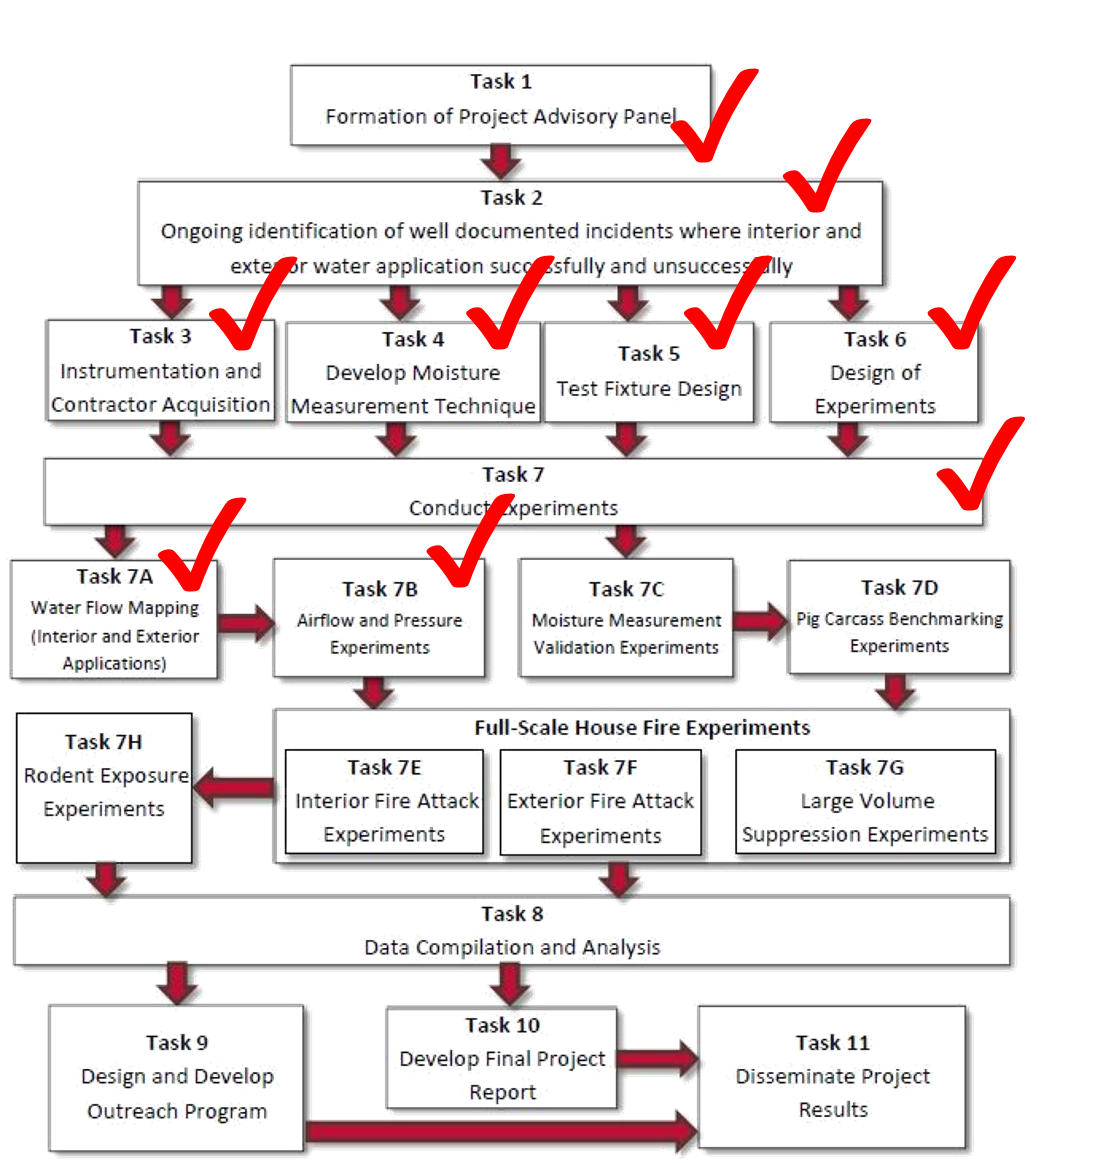
\includegraphics[width = 6in]{Figures/General/FlowChartChecks.png}
	\caption{Project Technical Plan Flow Chart}
	\label{fig:TechPlanChart}
\end{figure}

\clearpage

\item \bf{Task 1 – Formation of a Project Advisory Panel}
\normalfont
\vspace*{\baselineskip}

Task 1 will bring together an advisory panel of technical experts in the fire service; and fire service research field. An open application process will be administered to find fire service experts in fire stream application and training in fire attack methods. Representatives from organizations including: CFD (Chicago Fire Department), FDNY (Fire Department of New York), IAFC (International Association of Fire Chiefs), IAFF (International Association of Fire Fighters), NVFC (National Volunteer Fire Council), NIST (National Institute of Standards and Technology), and career and volunteer representatives from urban, suburban, and rural fire departments will be invited to participate. Invitations will also be extended to representatives of major fire service publications and training material publishers. This well rounded panel allows UL to ensure their research is directed to the target audiences and that the end product of the research is able to be easily disseminated into practice.
\vspace*{\baselineskip}

\item \bf{Task 2 – Incident Review}
\normalfont
\vspace*{\baselineskip}

Task 2 is to leverage our fire service advisory panel to conduct an extensive search to find examples of well documented successful and unsuccessful interior and exterior fire stream applications. This will be completed by monitoring fire service websites for videos and after action reports where there are defined flow paths and clear fire service fire attack actions. With approval of the fire department these incidents will be examined in detail to determine the impacts of fire stream type, flow, pattern and placement on the outcome of the incident, firefighter safety and victim injuries if applicable. Everyday the fire service is learning through their own experience and the experience of others through the means of sharing video. To make sure our experiments are tied in best with common fire service experiences we will identify trends in these incidents and tie the research results to the experience or beliefs gained from these incidents.
\vspace*{\baselineskip}

\item \bf{Task 3 – Test Supplies, Instrumentation and Contractor Acquisition}
\normalfont
\vspace*{\baselineskip}

Task 3 will allow for UL to acquire research supplies and instrumentation to complete this project. Instrumentation includes thermocouples to measure thermal conditions that potential victims or firefighters would be exposed to, differential pressure sensors and bidirectional probes to measure pressure and gas velocity throughout the test fixtures, bullet cameras to capture interior views of the test fixtures to provide visual evidence of conditions. Other test equipment such as data loggers, gas analyzers, thermal imaging cameras and video cameras were acquired from previous studies and will be utilized during this study. A contractor will also be selected to construct the test house structures using construction practices representative of what would be found in most neighborhoods across the country.
\vspace*{\baselineskip}

\item \bf{Task 4 – Develop Moisture Measurement Technique}
\normalfont
\vspace*{\baselineskip}

During this task different commercially available moisture measurement technologies will be examined for their ability to make moisture measurements in conditions that will be created in the full-scale house experiments. These conditions include elevated temperatures and a high density of particulate. This measurement will allow for the ability to map where steam travels in the structure to assess the impact of steam on fire victims and on fire service steam burns.

Several well established instruments exist to characterize the environmental conditions within a structure containing fires by measuring a variety of effluent gases along with temperature, heat flux and flow characteristics. However, the ability to measure moisture content in conditions applicable to describing fire environments, particularly after water has been applied to suppress the fire, is not presently available. The effect of measuring moisture at elevated temperatures is critical for hazard assessments for both firefighters operating within a structure and potential victims who are trapped in the structure. In the SFPE Handbook, Purser suggests that:  “… it is possible that the presence of water vapor may be an important neglected hazard in fires”, and, “Humid air, steam or smoke with a high thermal capacity of latent heat (due to vapor content or suspended liquid or solid particles) may be dangerous at temperatures of around 212~$^{\circ}$F (100~$^{\circ}$C), causing burns throughout the respiratory tract. It may be possible to predict the likely effects of hot-smoke atmospheres if thermal capacity or latent heat were measured.” 

Thus, the ability to measure moisture concentration in such environments is a critical avenue of research for firefighter safety as well as to fully understand the impact of tactical decisions on trapped victim safety. It is of particular importance to know the moisture content in the rooms adjacent to the fire room at the level of occupants crawling on the floor (1~ft above the floor) or on furnishings (3~ft above the floor). Based on past experimental results, the temperatures observed at these levels in rooms adjacent to the fire room are typically under 400~$^{\circ}$F.  

Commercially available moisture sensors have been developed recently for industrial process control, but these have not been studied for applicability to the live fire conditions. At the University of Illinois, Professor Dimitrios Kyritsis’ lab has advanced multiple techniques based on electrical and laser based measurements of gases during internal combustion engine operation that can be adapted to the sooty, dynamically changing live-fire environment. While there are a large number of techniques to measure moisture, most are inapplicable to the situation of high temperature moisture measurements in a combusting environment. Two techniques that could have use in these types of environments are infrared absorption techniques and electrical impedance techniques. There are two different methods to measure moisture using electrical impedance, resistive methods and capacitive methods. Both methods measure the relative humidity of the environment. Each method has its own set of advantages, with the resistive methods having a faster response time, while the capacitive methods can resolve relative humidity measurements all the way to 0\% RH. It is for this reason that the capacitive methods are most useful for this application, since at temperatures around 400 oF and volume percent of H2O under 10\%, the relative humidity will be under 1\% RH. Resistive methods do not accurately measure relative humidity under 5\% RH.  

Absorption spectrometry is another possible technique for measuring moisture content in harsh, high temperature environments. Water has several absorption bands in the near-infrared range, which allows the use of tunable diode lasers to measure the moisture content. With proper thermal and optical control of the laser source and sample train such a technique should be operable at temperature exceeding 1800~$^{\circ}$F, be able to operate in and compensate for sooty and smoky environments, and have a very rapid response time on the order of seconds. Such approaches have been utilized to perform in-situ analysis from controlled combustion and process exhaust systems. However, due to the nature of the live-fire experiments studied here, an extraction technique may have to be implemented. Such techniques will be designed and tested at the University of Illinois at Urbana-Champaign prior to the full-scale tests.
\vspace*{\baselineskip}

\item \bf{Task 5 – Test Fixture Design}
\normalfont
\vspace*{\baselineskip}

Task 5 is the design of the test fixtures to be used in the experiments. The main test fixtures will be two single family residential home (1200 ft$^2$ single story ranch house) to be constructed in UL’s Large Fire Facility. This is the near the same design built for the three previous ventilation research grants and will therefore allow continuity of previous results to expand our knowledge. One of the main test fixtures will be altered to constructed an open floor plan so that gas cooling can be analyzed in different volumes. The test fixture will be furnished with contents that is representative of common households and refurnished after each experiment. Additional test fixture details are provided in the Appendix.
\vspace*{\baselineskip}

\clearpage

\item \bf{Task 6 – Design of Experiments}
\normalfont
\vspace*{\baselineskip}

Task 6 is the design of the experiments. In this task UL’s project engineers will work closely with the advisory panel to ensure fire service concerns are addressed and that the results will be of great benefit to the end users. All experimental variables, equipment, personnel, infrastructure and other resources will be evaluated to determine the best set of experiments to get the most for the investment and provide the largest return to the fire community. Variables such as types of nozzles, flow rates, nozzle patterns, ventilation parameters, timing of tactics, ignition location, and fuel loading will be discussed and selected during a technical panel meeting.  
\vspace*{\baselineskip}

\item \bf{Task 7 - Conduct Experiments}
\normalfont
\vspace*{\baselineskip}

\subitem \bf{Task 7A:  Water Flow Mapping (Interior and Exterior Applications)}
\normalfont
\vspace*{\baselineskip} 

Methodology: Conduct a series of experiments in a compartment constructed to determine where water goes once discharged from fire department nozzles during a simulated interior fire attack and exterior fire attack. The ability to suppress a fire safely and efficiently is dependent on how much water absorbs energy from the fire and what surfaces are cooled. A combination of water mapping techniques that are commonly used for characterizing sprinkler sprays will be utilized to determine flow distribution. The compartment will be of similar size to the fire rooms in the full-scale fire experiments so that the results can be linked.

Water will be flowed utilizing common fire department nozzles with 3 patterns (combination nozzle in a straight stream pattern, combination nozzle in a narrow fog pattern and a smooth bore nozzle pattern). Different nozzle techniques that are commonly taught to firefighters and utilized in practice will be evaluated such as circular motions, z patterns, flowing off the ceiling and flowing ahead. Common flow rates for each nozzle will be used during the experiments. We will also calibrate our remote water delivery method that will be utilized during Tasks 7E and 7F to distribute the water in a repeatable manner to what would be done by firefighters. Several experiments will be done in triplicate to examine repeatability.  

Measurements: The actual delivered density apparatus (described later) will be used to determine water distribution, video cameras will be used to document the nozzle techniques and gross water distribution. Data from this Task will be analyzed and used to design the experiments described in Task 7E, 7F, and 7G.
\vspace*{\baselineskip}

\subitem \bf{Task 7B:  Air Flow and Pressure Experiments}
\normalfont
\vspace*{\baselineskip}

Methodology: Conduct air flow and pressure experiments in the test fixtures prior to the introduction of any fire. Different hose streams and nozzle movement techniques entrain different amounts of air which can greatly impact fire dynamics, firefighter safety and victim survivability. The same nozzles, stream types and nozzle techniques will be used as Task 7A and the amount of air flow created and pressures generated in the structure will be measured. Different flow paths will also be established to see their impact such as having a ventilation point ahead of the hose-line and having no ventilation opening ahead of the hoseline. We will also examine air movement generated by 1 ¾ in., 2 ½ in. hand-lines and flows from master-stream devices (deck gun and ladder pipe).

Measurements: During each of these experiments, velocities will be measured with anemometers and bidirectional probes attached to differential pressure gauges. Pressures will be measured with differential pressure gauges and HVAC air balancing measurements will be made. This data will allow for the analysis of air movement and its impact on fire growth measured in Tasks 7E and 7F.
\vspace*{\baselineskip}

\subitem \bf{Task 7C:  Moisture Measurement Validation Experiments}
\normalfont
\vspace*{\baselineskip}

Methodology: The candidate moisture measurement techniques identified in Task 4 will be validated by this series of experiments. A bench scale apparatus will be designed and constructed that will allow the team to carefully calibrate moisture concentrations at temperatures up to 500~$^{\circ}$F and in the presence of potential confounders such as typical fire effluent gases and dense smoke conditions. A closed loop flow bench will be designed with a radiative heating element and moisture injection ports allowing adding controlled volumes of moisture to initially dry room air. These ports will also allow controlled metering of CO and CO2 as well as fire smoke effluent collected from live-fire burn experiments.

Measurements: Moisture percentage will be measured and compared against controlled ambient conditions. Initial measurements will be made in a controlled environment with known temperature and moisture concentrations up to 500~$^{\circ}$F, (max 3~ft temperatures in bedrooms found in the Vertical Ventilation Study (source***)). After validation in these environments, a controlled concentration of potential confounders will be added to the test bench included typical fire gases (CO2, CO) and varying soot concentrations.
\vspace*{\baselineskip}

\subitem \bf{Task 7D:  Pig Carcass Benchmarking Experiments}
\normalfont
\vspace*{\baselineskip}

Victims trapped within a structure face the risk of thermal burn injuries, particularly with unprotected skin. Suppression activities by the Fire Service can reduce this hazard by removing the heat source producing these dangerous conditions, however, the additional risks encountered by the conversion of water to steam must be studied. The risk for moisture related skin burns is likewise present for firefighters applying water to burning materials from inside the structure. While firefighting PPE provides a significant measure of protection, burn injuries are still a significant hazard during interior firefighting operations.

The dangers of thermal injury from exposure to heat and products of combustion and time-temperature characteristics required for skin burns has been researched for several years. Typical studies involve exposing skin to a controlled thermal exposure and the time to an outcome, such as dermal or epidermal temperature changes or visual indications of damage. The synergistic effect of elevated temperature and moisture content on skin is conceptually understood due to the large latent heat and partial pressure of water at temperatures above 140~$^{\circ}$F. However, the effect of suppression tactics and the rapidly changing transient nature of exposure during this time frame (ambient temperature reducing, moisture content increasing) on risk for skin burns has not been measured in response to realistic fire suppression experiments. 

Most commonly, porcine skin is used as a surrogate for human skin in burn studies (source**) as pig skin is more human like than any other readily available animal (source***). Furthermore, epidermal and dermal thicknesses for 3-4 month old swine are similar to an average human is estimated to be 70~µm, and 2-3~mm. Pig carcasses have been successfully utilized in place of live animal studies in part because the water loss from the skin of a live pig does not differ significantly from a carcass (source**).

Methodology: In order to better understand burn injuries to both firefighters and potential occupants pig carcasses will be placed in various target rooms at different locations (1~ft and 3~ft from the floor) near the moisture sampling measurements during the house fire experiments. Pig carcasses will be obtained through the University Of Illinois College Of Veterinary Medicine after they have completed their research tasks at the University. The 3-4 month old pigs will be of similar weight and have skin thickness (epidermal layer ~60-80~µm, dermal thickness of 1-3~mm) that is comparable to human skin and can be analyzed as a surrogate for potential human skin damage. Prior to inclusion in the live-fire structure, samples will be exposed to varying levels of radiant and convected heat with controlled moisture content to establish a baseline for comparison of damage as a function of exposure.  

Measurements: Thermocouples will be sewn onto the skin surface and under the pig’s dermal layer using sutures to measure temperature gradient and establish the time line for first degree (skin surface at 113~$^{\circ}$F) and third degree (sub-dermal temperatures reach 113~$^{\circ}$F). In the scenarios where sections of the pig will be covered by firefighting PPE, temperature and relative humidity (to measure penetration of moisture through the PPE) will be measured on the exterior and interior of the clothing in the same area. Using the instrument developed and validated in Task 7C moisture concentration will be measured in the immediate vicinity of the exposed pig. Skin damage will be well documented visually for comparison with the carcasses utilized in Tasks 7E-G.
\vspace*{\baselineskip}

\subitem \bf{Task 7E:  Interior Fire Attack Experiments}
\normalfont
\vspace*{\baselineskip}

Methodology: A series of 12 full-scale house fire experiments will be conducted with simulated interior fire attack. The house will be furnished with modern furnishings and each experiment will have identical content.  A fire will be ignited in the master bedroom and the flow path will be altered to simulate scenarios that the fire department would arrive to or that would be created by fire department operations. The first 6 experiments will examine fire department arrival to a closed house with a ventilation limited fire. The front door will be opened creating a flow path. This will be repeated 5 times, utilizing 2 different hose streams, a controlled door, a coordinated ventilation opening, and once with no water application.  

Five victim locations will be instrumented and the flow path the attack crew would be advancing through will be instrumented to examine conditions that the crew would be exposed to. The hosestream will be applied utilizing a monitor nozzle that will be able to advance on a set of tracks and will be programmed to flow the desired pattern and motion. The second set of experiments will add a second flow path by ventilating the master bedroom window. This will increase the size of the fire but will provide a low pressure point opposite of the attack crew. This will be repeated 5 times with two different hose stream patterns, two different hose line advances, and once with no water application until the front door flow path closes up and fire extends out of the front door. A third set of experiments will add a third flow path through Bedroom 2. Again 2 different hose stream patterns will be examined, two difference advances will be tested, and one experiment where no water is applied until fire extends out of the front door of the structure.

Measurements: Measurements will be made to examine the fire dynamics in the test fixture, the exposure to firefighters in the flow path and to potential victims in several locations. The test fixture will be instrumented to measure temperature in every room, gas concentrations, pressure, gas velocity, thermal imaging and digital video. These measurements will allow for quantification of fire behavior, the impact of the water application and tenability for firefighters and occupants. Five victim measurement packages will be placed in the test fixture.  The packages will consist of temperature measurements at multiple elevations, gas concentration measurements (oxygen, carbon monoxide and carbon dioxide), heat flux with water conditioned to 98 degrees to get more accurate heat transfer to skin, an instrumented pig carcass, a moisture measurement device and a video camera. 
\vspace*{\baselineskip}

\subitem \bf{Task 7F:  Exterior Fire Attack Experiments}
\normalfont
\vspace*{\baselineskip}

Methodology: A series of 6 full-scale house fire experiments will be conducted with simulated offensive exterior fire attack. A fire will be ignited in the master bedroom and the flow path will be altered to simulate scenarios that the fire department would arrive to or that would be created by fire department operations. The first 4 experiments will examine fire department arrival to fire extending out of the master bedroom window. Water will be applied through the window, utilizing 3 different hose streams. Five victim locations will be instrumented to examine conditions that they would be exposed to. The hose stream will be applied utilizing a monitor nozzle that will be programmed to flow the desired pattern and motion. The second set of experiments will add a flow path by ventilating the Bedroom 2 window. This will increase the size of the fire and will allow it to begin to spread into Bedroom 2. This will be repeated 3 times with three different hose stream patterns and once with no water application. A third set of 2 experiments will ignite the fire in the master bedroom and Bedroom 2 with both of their windows open (Figure 10). Once fire is extending out of both bedroom windows 2 different hose stream patterns will be examined by flowing water into the master bedroom window.

Measurements: Same measurements as Task 7E, Interior Fire Attack Experiments.
\vspace*{\baselineskip}

\subitem \bf{Task 7G:  Large Volume Suppression Experiments}
\normalfont
\vspace*{\baselineskip}

Methodology: A series of 8 experiments will be conducted that are the same as the first 8 interior fire attack experiments with the exception that all of the interior walls in the test fixture will be removed except for the walls to the master bedroom (Figure 11 and Figure 12).  This increased volume will allow for the analysis of gas cooling as a result of indirect attack in an open floor plan when the fire can not be accessed with the hose stream without crawling into the structure through the flow path. The fire will be allowed to develop until temperatures in the large volume would require an advancing attack crew to cool the upper gas layer in order to advance to the bedroom fire.  The advancing crew will be simulated just as in Task 7E so that the 2 configurations can be compared, compartmented floor plan versus modern open floor plan.

Measurements:  The test fixture will be instrumented to measure temperature in every room, gas concentrations, pressure, gas velocity, thermal imaging and digital video. Four victim locations will be instrumented to examine conditions that they would be exposed to. These measurements will allow for quantification of fire behavior, the impact of the water application and tenability for firefighters and occupants. The data will be analyzed and compared to the compartmented measurements from Task 7E.
\vspace*{\baselineskip}
 
\item \bf{Task 8 – Data Compilation and Analysis}
\normalfont
\vspace*{\baselineskip}

Task 8 is the compilation and analysis that will be conducted by UL engineers to make the data usable by the fire community. The data will be organized in graphs that will be reviewed by the technical panel in preparation for the final report and the online training program. The focus of the analysis will be to calculate tenability conditions for potential victims and firefighters during each of the scenarios. In addition, tactical considerations will be developed in conjunction with the fire service advisory panel. Each of these considerations will be supported by data, experimental video evidence and actual fire incidents documented in Task 2 and incorporated in the technical report and outreach program.
\vspace*{\baselineskip}

\item \bf{Task 9 – Design and Develop Outreach Program}
\normalfont
\vspace*{\baselineskip}

In task 9, UL engineers will work with instructional designers to produce an interactive training program for the fire community. The final program will be shared via the www.ULfirefightersafety.com website, www.Modernfirebehavior.com website, and UL FSRI Social media accounts free of charge to the fire service. The course will be consistent with previous courses developed by UL as shown in the figures below. The course will contain data, pictures, video and professional narration and allow firefighters of all levels to navigate through the course at their own speed. This program will include linkages to tactical considerations learned from the previous three studies on horizontal, vertical and positive pressure ventilation and the Governor’s Island experiments completed in partnership with FDNY and NIST.
\vspace*{\baselineskip}

\item \bf{Task 10 – Develop Final Project Report}
\normalfont
\vspace*{\baselineskip}

Task 10 is the development of the final report that details all of the experiments and results. The report will be provided to DHS and made publicly available via UL’s website for the fire service, www.ULfirefightersafety.com to serve as a reference for future research. The tactical considerations developed with the technical advisory panel will be a focus within the report. A fire service summary report will also be written and disseminated that includes critical information for firefighter safety.
\vspace*{\baselineskip}

\item \bf{Task 11 – Disseminate Project Results}
\normalfont
\vspace*{\baselineskip}

Task 11 is the dissemination of the research results. Results are shared by presenting in venues such as the National Fire Protection Association Annual Conference, Fire Department Instructors Conference, International Association of Fire Chiefs Fire Rescue International, and the International Association of Fire Fighters Annual Conference. These venues provide a large number of attendees from the fire service and research communities and are a formal means to disseminate the results of the study. Additional dissemination will include publication in fire service trade magazines and peer reviewed journals. As with previous outreach results, videos and presentation content will be made available at request to be used for local dissemination and for train the trainer programs. Continued dissemination is achieved by making the final project report and online training program available via UL’s websites for the fire service, www.ULfirefightersafety.com and www.Modernfirebehavior.com. We will also share project results on our and our partners social media channels, Facebook, Twitter, Youtube and our Fire Engineering Radio Show, “Research to Tactics.”
\vspace*{\baselineskip}

\end{itemize}

\clearpage

\subsection{Limitation and Scope}

The fire attack study is not intended to establish which methods of fire attack are more effective when compared to others. More specifically, Part I of the study is not intended to dictate tactics or the purchasing of one type of nozzle over another. The purpose is to quantify the amount of air entrainment in nozzles given certain parameters as well as determine where water is distributed within a compartment. This is all without fire involvement in order to provide a baseline understanding before moving forward with the remainder of the study. This baseline knowledge is intended to bridge the gap in the fire service understanding about the use of various nozzles, application patterns, and advancement techniques in specific scenarios. Knowing how hose streams affect air movement and how water is distributed can allow for better decision making capabilities across the fire service when it comes to equipment purchasing and use during an actual emergency incident.

When analyzing the air entrainment and water distribution, equipment from various manufacturers was tested. For the purpose of the study, the companies will be referred to as Manufacturer 1, Manufacturer II, and Manufacturer III. The air entrainment experiments yielded results that showed little to no difference among the various manufacturers. Therefore, a single manufacturer was chosen for the remainder of Part I of the study.

The intent of the air entrainment experiments was to determine how much air nozzles entrain. This involved several components:

\begin{itemize}
	\item Does the amount of air entrainment vary dependent on manufacturer given set flows/pressures?
	\item Does adjusting the flows/pressures of the nozzles effect air entrainment? 
	\item Does the nozzle type (smooth bore versus combination) effect air entrainment? 
	\item Does the application pattern effect air entrainment (fixed, sweeping, O, T, Z, inverted U)?
	\item Does the distance from a ventilation opening effect the air entrainment?
	\item How do different building geometries and compartment layouts effect air entrainment?
\end{itemize}

Additionally, the intent of the water distribution experiments was to determine where water goes within a compartment. In order to answer this question, the tests considered the following:

\begin{itemize}
	\item Does interior versus exterior attack effect water distribution?
	\item Does the hose stream angle effect water distribution?
	\item Does adjusting the flows/pressures of the nozzles effect water distribution? 
	\item Does the nozzle type (smooth bore versus combination) effect water distribution? 
	\item Does the application pattern effect water distribution (fixed, sweeping, O, T, Z, inverted U)?
	\item Does the distance from a ventilation opening affect the water distribution?
	\item How does a first floor exterior attack effect the water distribution when compared to a second floor exterior attack?
\end{itemize}

Each and every fire department across the world utilizes different personal protective equipment, firefighting equipment, staffing levels, apparatus, standard operating procedures, and tactics. Additionally, no two fires are identical as well. Thus provides a challenge for researchers when evaluating what can be varied versus held constant during testing. For the purpose of these experiments we utilized the same structure throughout all of the air entrainment experiments. The water distribution testing utilized another structure, which also remained the same for the duration of those experiments. The only component of the firefighting equipment that was varied among the tests was the nozzle, and sometimes the hose line size. The hose line was either 1 3/4~in or 2 1/2~in in diameter and was always 200~ft in length. By creating some aspects that were not varied and by bounding other variables, we ensured that all aspects of the air entrainment and water distribution were examined as a baseline for further future evaluation in different structures with different conditions.

\clearpage

\section{Project Technical Panel}

In order to better design and implement the experiments for the Fire Attack study, UL - FSRI has gathered a group of fire service experts from across the world with knowledge in fire suppression and the impact of interior and exterior fire streams. Announcements were made regarding the open application period for firefighters of all ranks and experience to participate in the study. After the application period closed, the UL - FSRI team evaluated the responses for those with training and experience specifically related to fire suppression operations. In addition, the team selected applications which encompassed a wide variety of ranks and geographic areas to ensure that the majority of the tactics used in the United States, including some international presence, would be represented. The panel members selected best represent the firefighters' experience with fire attack and the impact on safety and survivability.

\begin{figure}[H]
	\centering
	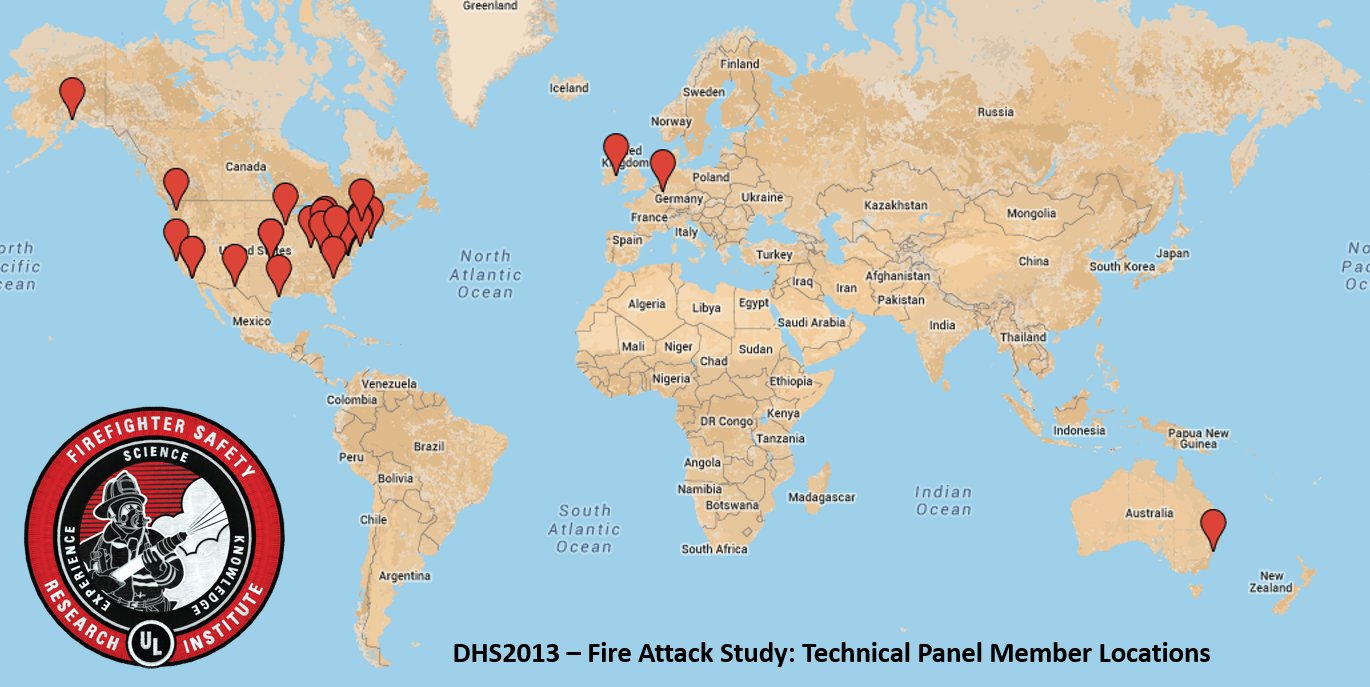
\includegraphics[width = 5in]{Figures/General/Technical_Panel_Logos.png} 
	\caption{Fire Attack Technical Panel Member Locations}
	\label{fig:PanelLocatoins}
\end{figure} 

\clearpage

The individuals below provided direction for the project, assisting in planing the experiments, witnessing the testing, and developing tactical considerations. Their tireless support and effort make this project relevant to the fire service across the world. 

\renewcommand{\arraystretch}{1.5}

\begin{table}[H]
	\centering
	\caption{Fire Service Technical Panel}
	\begin{tabular}{|c|c|}
		\hline
		\bf{Name} & \bf{Fire Department} \\ \hline \hline
		Chad Green & Anchorage Fire Department \\ \hline
		Chad Christensen & Los Angeles County Fire Department \\ \hline
		Dennis Legear & Oakland Fire Department \\ \hline
		Jerry Bedoya & Los Angeles City Fire Department \\ \hline
		Tony Carroll & Washington DC Fire Department \\ \hline
		Jordan Mohr & Sedgwick County Fire District 1 \\ \hline
		Samuel Hittle & Wichita Fire Department \\ \hline
		John Gallagher & Boston Fire Department \\ \hline
		Josh Hummel & Howard County Department of Fire and Rescue Services \\ \hline
		Matt Carrigan & Montgomery County Fire and Rescue Service \\ \hline
		Robert Shinske & Detroit Fire Department \\ \hline
		Kelly Hanink & Eden Prairie Fire Department \\ \hline
		Jason Floyd & Las Cruces Fire Department \\ \hline
		Jerry Knapp & West Haverstraw (NY) Fire Department \\ \hline
		Ray McCormack & Fire Department of New York \\ \hline
		Jacob Hoffman & Toledo Fire Department \\ \hline
		Steve Pegram & Goshen Township Fire and EMS \\ \hline
		Danny Doyle & Pittsburgh Fire Department \\ \hline
		Nick Martin & Columbia Fire Department \\ \hline
		Albert Castillo & Houston Fire Department \\ \hline
		Aaron Fields & Seattle Fire Department \\ \hline
		Steve Brisebois & Montreal Fire Department \\ \hline
		Hans Neiling & Zuid Limburg Fire \\ \hline
		John McDonough & New South Wales Fire Department \\ \hline
		John Chubb & Dublin Fire Brigade \\ \hline		 		  
	\end{tabular}
	\label{tab:TechPanelList}
\end{table}

\clearpage

\section{Previous Literature}

At the start of the study, a literature review was performed to identify and analyze the following:

\begin{itemize}
	\item Previous research in the field of air entrainment, water distribution, and fire suppression
	\item Previous research into victim burns and survivability in fires
	\item Both past and current fire suppression tactics 
	\item Knowledge gaps in fire suppression operations (choice of tactics, myths, traditions, etc.) 
\end{itemize}

The following section outlines some of the material as it relates to the fire attack study. The literature review encompassed past research work, various articles in fire service publications, fire service training manuals, fire department standard operating procedures, as well as line of duty injury/death reports to highlight some of the critical areas of information which drove the project at hand.

\subsection{Literature Overview}

Hose, nozzles and water have been used by the fire service for hundreds of years. Despite their frequent use, there has been little scientific research conducted on the effective use of these tools for fire suppression. It is common in the fire service to find discussions about which nozzle is better or which flow rate is required for what sized fire but this is based on experience and usually not science. 

In 1950 Chief Lloyd Layman presented a paper titled “Little Drops of Water” at the Fire Department Instructors Conference. He introduced what he called indirect method of attack to suppress interior building fires by using the heat absorbing properties of expanding and condensing steam, produced in great quantities by fog streams. The conclusions were based on Coast Guard experiments that Layman was in charge of conducting at the Coast Guard Firefighting School at Fort McHenry in Baltimore, MD. Layman continued his experiments after he returned to his position as fire chief in Parkersburg, WV where he applied his tactic in building fires.  This research had a very large impact on the fire service and their suppression techniques to this day. 

Throughout the 1950’s a National Committee began conducting experiments to collect data on the growth and behavior of interior fires and how to most effectively suppress them. Keith Royer and Bill Nelson were members of this committee, and as the heads of the firemanship training program at the Iowa State University’s Engineering Extension, they collected and analyzed data from hundreds of experimental fires. Through this research the fire service was taught about fire behavior and how to suppress fire with a combination fire attack. They examined the amount of heat generated by common fuels, the heat absorbing capacity of water, the impact of compartment volume during suppression and they developed the Iowa formula. The Iowa formula or critical rate of flow formula is still used today and it determines the amount of water needed to control a fire in the largest open space within a structure by dividing the cubic foot volume of the space by 100.

While the physics of fire development has not changed over time, the fire environment for specifically the single family home has evolved. Several factors including home size, geometry, contents and construction materials have changed significantly over the past 50 or more years. Each of these factors has impacted firefighter and occupant safety. Faster fire propagation, shorter times to flashover, rapid changes in fire dynamics and shorter escape times all impact fire service suppression techniques and effectiveness. Many of the variables in Royer and Nelson’s analysis have changed and more research is needed to see how suppression techniques used in the 1950’s with 1950’s fuel loads and firefighting tools translates to today’s firefighter safety and effectiveness.

Beginning in 1994, the Naval Research Laboratory carried out a series of full-scale fire experiments to compare straight stream attack versus fog pattern attack. These experiments were conducted on the Navy ship ex-USS Shadwell with a fire volume of approximately 110~m$^3$. In these experiments one 60 degree fog pattern was applied at a 45 degree angle into the smoke layer. They examined cooling effects, steam generation and thermal layer disruption. Their experiments examined shielded and non-shielded fires and concluded that using fog to cool the upper layer was more effective and safer than straight stream attack when the fire could not be attacked directly and the firefighters heart rates and body temperatures were lower utilizing the fog attack.

In 1998 NIST conducted a series of experiments to demonstrate the suppression effectiveness of water-based firefighting agents. This was a step toward creating test procedures to determine suppression effectiveness to develop a standardized test method for evaluating the fire fighting effectiveness of water and other agents. This study provides preliminary data upon which firefighting effectiveness test may be developed by it suggests additional research on application technique, tests reflective of the complexities found in firefighting and experiments involving structural-fire suppression.  

In 2002, The National Research Council of Canada conducted a literature search on 3D water fog techniques for firefighting. It discusses the impact of water fog characteristics associated with properties of the nozzle (e,g,, droplet size, momentum, flow rate, spray angle and pattern) and discharge techniques (e.g., discharge angle, and discharge duration related to the burts) on performance of the 3D water fog technique are discussed. This technique is to supplement a direct attack by controlling the environment the firefighters are in until they are in a position to apply water directly to the fire. Opponents of flowing water into smoke have concerns that include: (i) effectiveness of controlling the fire, compared to traditional straight stream attack; (ii) possible disruption of the thermal balance; (iii) possible generation of a large amount of hot steam that produces burn injuries to firefighters; and (iv) the performance of this technique is complex and requires extensive training. Advocates of this technique have attempted to respond to these concerns but very limited experimental studies have been undertaken do to complexity of the problems. Application techniques and fire conditions on the the performance of fog technique is not well studied and therefore there are little guidelines and adoption will be greatly limited.

Several theoretical studies had been conducted that examine droplet size and their ability to suppress fire gases. For example, when droplet diameter is reduced from 1000 nanometers to 100 nanometers the total surface area increases 10 times from 6 m2 to 60 m2 for 1 liter of water. Since these smaller droplets evaporate sooner, others have examined the lifetime of the droplet to determine how far it can travel based on temperature of the surrounding gases and droplet size. Further complicating this theory is that droplets all have an impact on each other as they turn to steam. Residence time can be further reduced compared to an individual droplet, because leading droplets impart forward momentum to the surrounding gas, reducing the air drag on the following droplets and resulting in better penetration. In 2010, the University of Maryland examined spray characteristics from fire hose nozzles. They examined the breakup of a smooth bore nozzle utilizing techniques such as shadowgraphy and a patternator and concluded that more research was needed to fully understand the water spray from fire hose nozzles.  

In 2000, Lund University examined the demand for extinguishing media in manual firefighting. They examined critical flow rates required to suppress fires by reviewing available literature and conducted a series of experiments that examined suppression of wood pallets at a fire training academy. They examined the five ways that water can be applied during fire extiguishment, on hot gases, on flames, on burning fuel, on fuel that is not yet burning and on hot surfaces. They highlight that what is most effective against the fire is not necessarily best for the firefighters since there are other constraints during firefighting operations such as limited air supply and multiple priorities. The optimum flow rate corresponds to an optimum control time, a control time that gives the lowest total demand for resources. Most of the current data for optimum water flow rate include experiments utilizing wood cribs or pallets, but not todays synthetic fuel loads in actual structures.  These studies also did not investigate the effect of flow paths or the impact of steam generation on firefighters or victims.

In 2003, a fire service group at the Rockland County (NY) Fire Training Center conducted a series of tests in their concrete training building. They measured the amount of air moved by solid bore and combination nozzles using common fire ground methods. They concluded that air volumes moved by smooth bore nozzles and combination nozzles in the straight stream setting are very similar if not the same, and that combination nozzles in the fog pattern move significant amounts of air which can over pressurize the fire area and send steam over the attack crew even with a ventilation opening opposite the attack crew. These tests were performed either with no fire or with a training fire but which are very different than actual fire conditions. Their tests do provide a good range of airflows that can be expected in our experiments. The authors state, “Our nozzle testing program was not as controlled and as precise as we would have liked.” They also did not have measurement devices that were able to accurately measure air flows from a fog pattern.  

The Firefighting Technology Group at NIST has a current project that is examining hose streams. This project examines a variety of fire fighting hose stream characteristics related to flow, distribution and thermal impact from both solid and fog stream nozzles. A series of real scale, laboratory based experiments have been started to look specifically at the water discharge and distribution characteristics, the impact of hose streams on a hot gas layer in a compartment, the impact of hose streams on gas flows through multi-compartment structures, and the suppression effectiveness on burning piles of wooden pallets. The proposed project will build on their results by utilizing real-scale structures with common residential fuels and making additional measurements to better characterize the impact of flow path, nozzle technique and steam generation on fire dynamics, firefighter exposure and occupant survivability.

\subsection{Fire Service Publications}

[MIKE]

\subsection{Fire Service Training Manuals}

[MIKE]

\subsection{Firefighter Line of Duty Deaths}

[MIKE]

\subsection{Research Work}

[MIKE]

\clearpage

\section{Instrumentation}

In order to obtain the results for Part I of this study, sensors were installed in the test fixtures to record measurements throughout the experiments. The instrumentation used varied between the air entrainment and the water distribution testing. The instrtuments, and associated uncertainty, used for each test series is outlined below.

\subsection{Air Entrainment}

To determine the amount of air entrained in nozzles, gas velocity was obtained through the use of an array of bi-directional probes in conjunction with differential pressure transducers and inconel thermocouples. The bi-directional probe was constructed of stainless steel and features a `high' side and a `low' side which travel back to a pressure transducer that evaulates the differential pressure from ambient pressure. The iconel thermocouples were placed in-line wtih the bi-directional probes to ensure that the measurements were recorded at the same location. The iconel thermocouple was a 0.063~in. diameter type KSL iconel 600 sheathed grounded junction with a type K, 24~gauge glass/glass insulation lead. The differential pressure transducer was a Setra Model 264 with a range of ±1.0~in. WC (±248.8~Pa). The uncertainty given by the manufacturer is 1\% or 1.2~Pa. The configuration had a velocity range of ±24.2~m/s (±54~mph). The pressure transducers were configured in groups of 6, contained in a single plastic box with connections for pressure, temperature and power (Figure \ref{fig:Gas_Velocity_Measurements}a). Five probes were installed in openings where velocity measurements were taken, centered horizontally in the opening (Figure \ref{fig:Gas_Velocity_Measurements}b). Velocity measurement with this configuration was determined to have an uncertainty of ±5\% \cite{BDPInPoolFires}.

\begin{figure} [H]
	\centering
	\begin{tabular}{c c}
		\subfloat[Pressure Transducer Box]{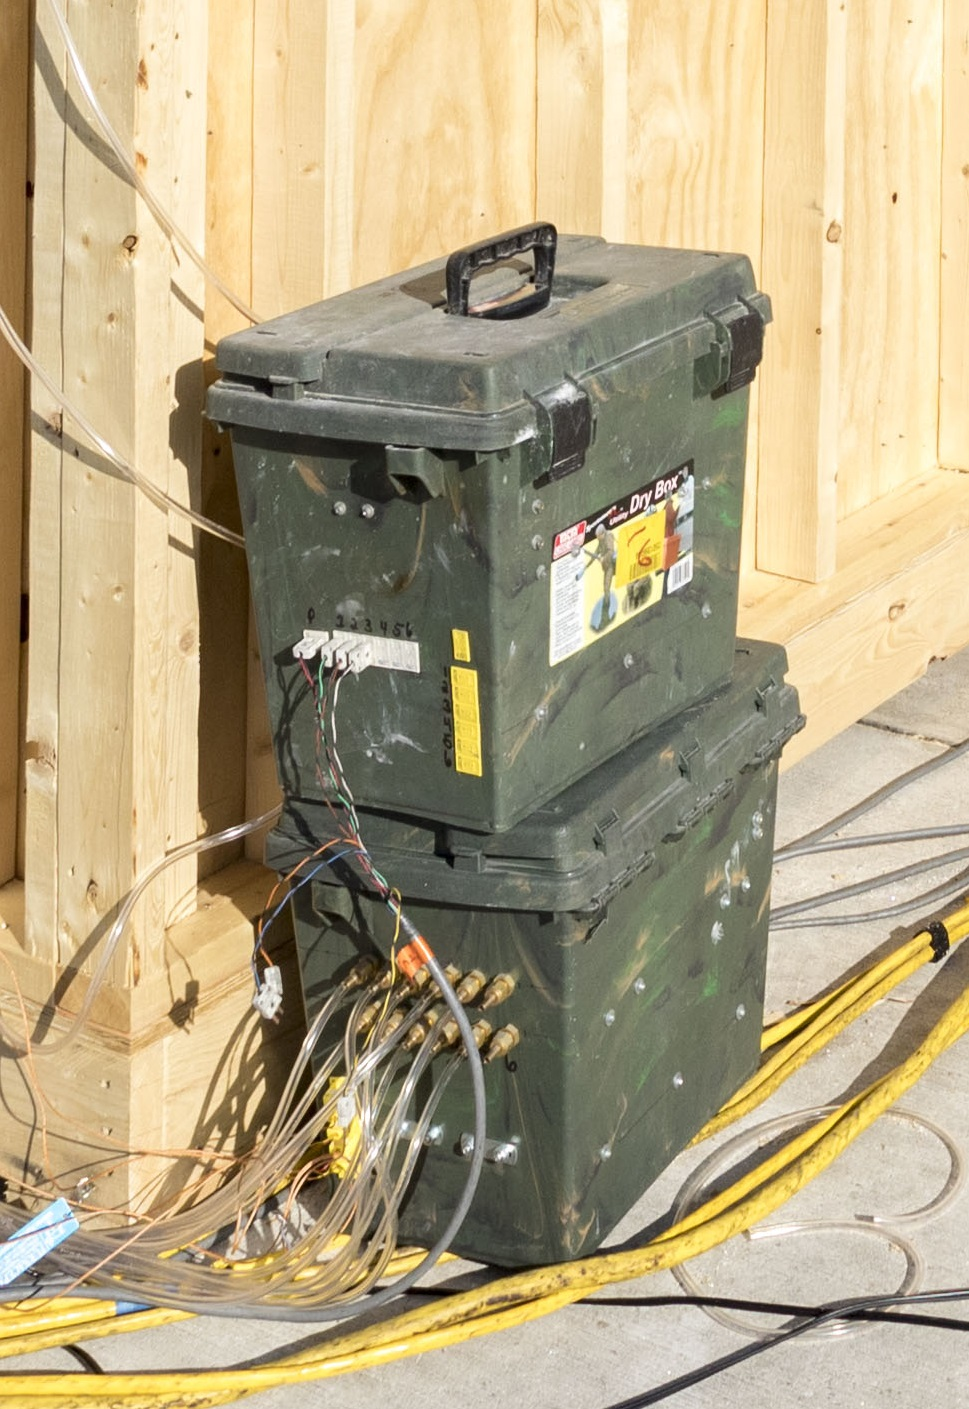
\includegraphics[height = 2.5in]{../0_Images/Instrumentation/PressureBox.jpg}} &
		\subfloat[Bi-Directional Probe Array]{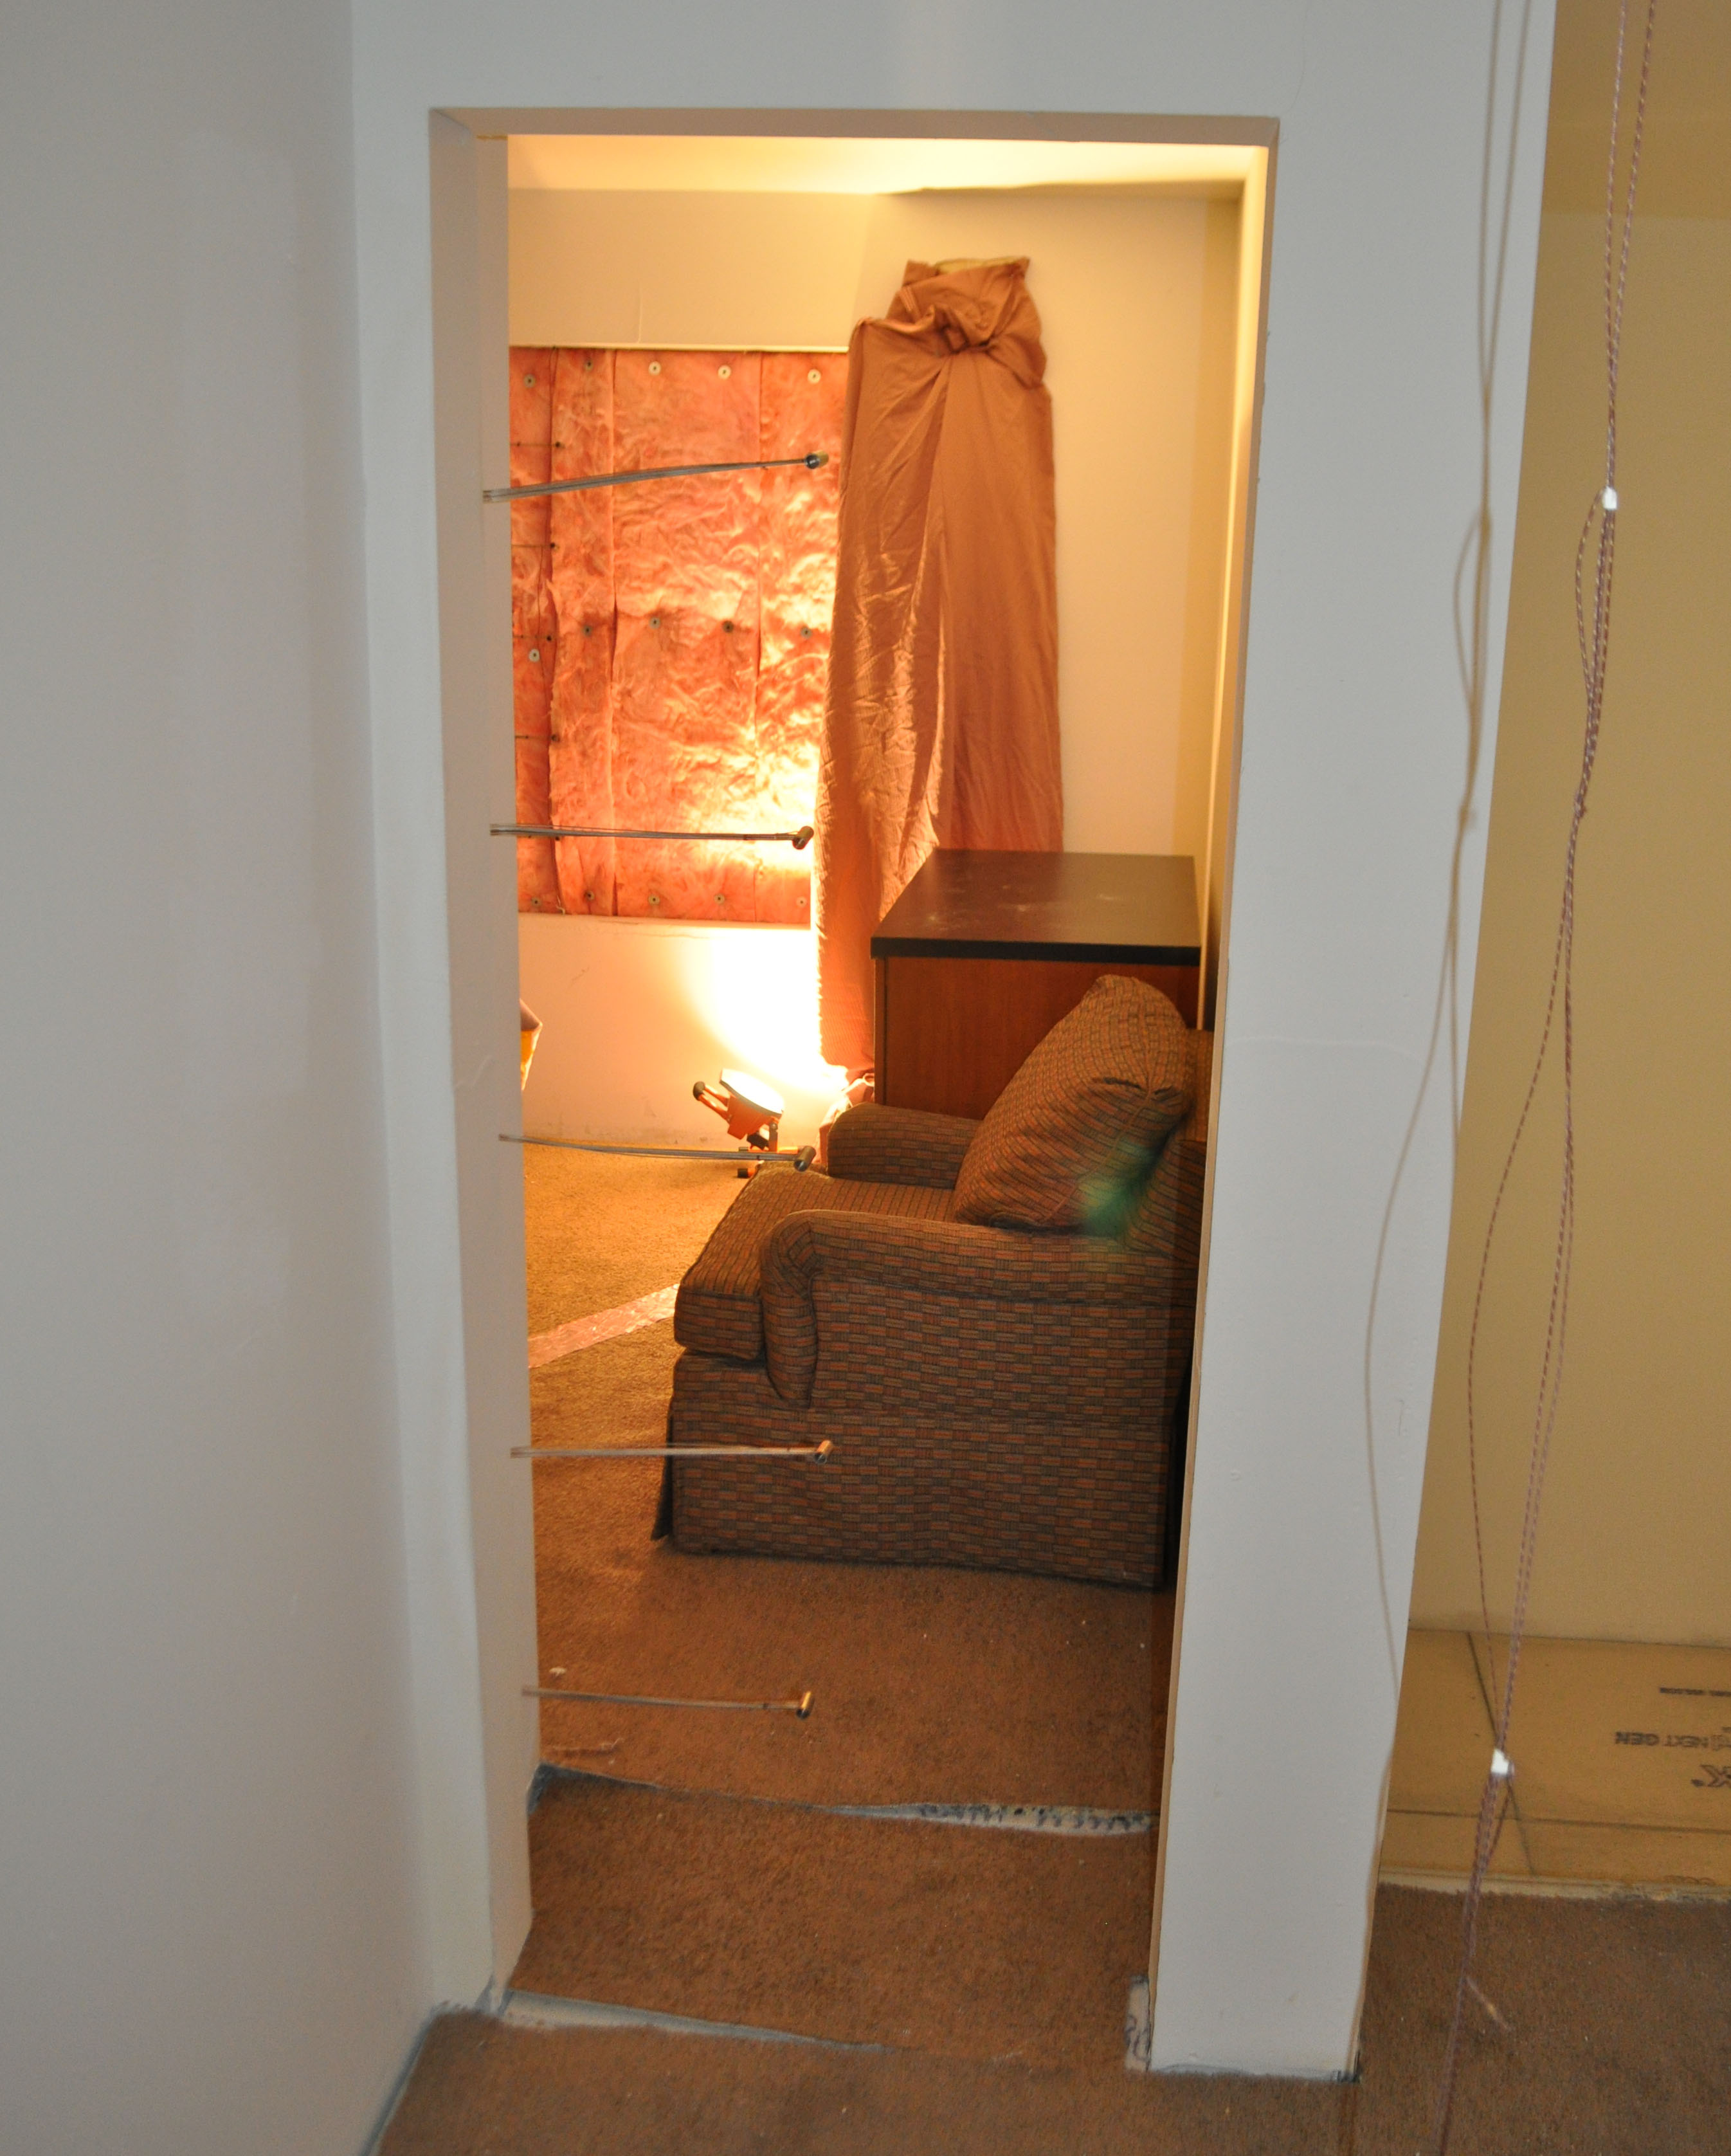
\includegraphics[height = 2.5in]{../0_Images/Instrumentation/BDPArray.jpg}} \\
	\end{tabular}
	\caption{Gas Velocity Measurements}
	\label{fig:Gas_Velocity_Measurements}
\end{figure}

\clearpage

Standard video was obtained through the use of BoschVTC-206F03-4 video cameras (Figure \ref{fig:BullettCam}). All cameras were recorded via Samsung DVR.

\begin{figure} [H]
	\centering
	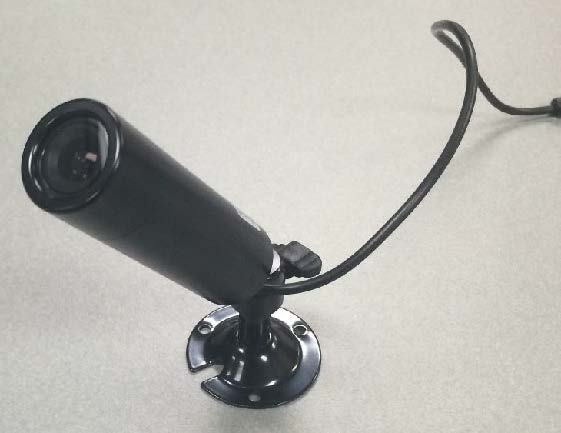
\includegraphics[width = 3in]{../0_Images/Instrumentation/BullettCam.jpg}
	\caption{Bullet Camera}
	\label{fig:BullettCam}
\end{figure}

All data was logged through the use of a national instruments data acquisition system incorporating a SCXI-1001 chassis with 8 SCXI-1102C 32-Channel modules (Figure \ref{fig:DataSystem}). The system is configured for a total of 256 channels capable of reading values between 0-10 volts DC. Values are recorded once a second and translated to quantities of interest through the use of LabVIEW software specifically programmed for use with the system.

\begin{figure}[H]
	\centering
	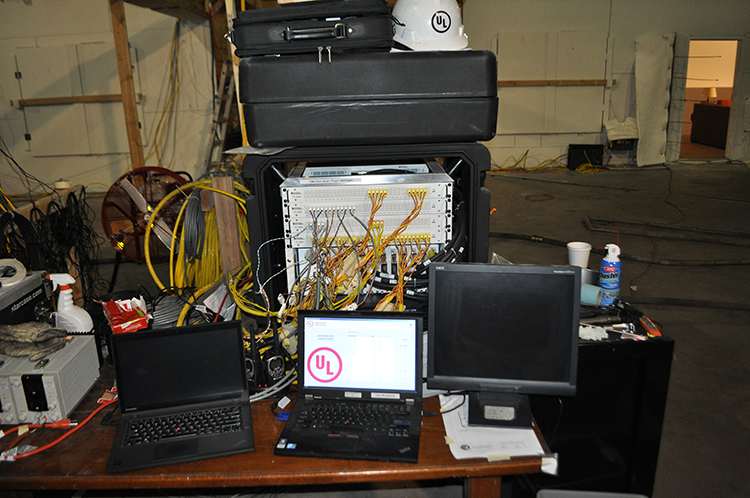
\includegraphics[width = 4in]{../0_Images/Instrumentation/DataSystem.jpg}
	\caption{Data Acquisition System}
	\label{fig:DataSystem}
\end{figure}

\clearpage

\subsection{Water Distribution}

UL operates a fire sprinkler spray density measurement instrument known as the Actual Delivered Density (ADD) apparatus. The first prototype of the apparatus was built at Factory Mutual in mid-1980’s, in order to enable manufacturers to design sprinklers that are effective at ever-increasing commodity storage heights \hl{[1, 2]}. The UL ADD apparatus, constructed in 2003, represents the 3rd generation design within the sprinkler industry. 
 
\begin{figure}[!ht]
	\centering
	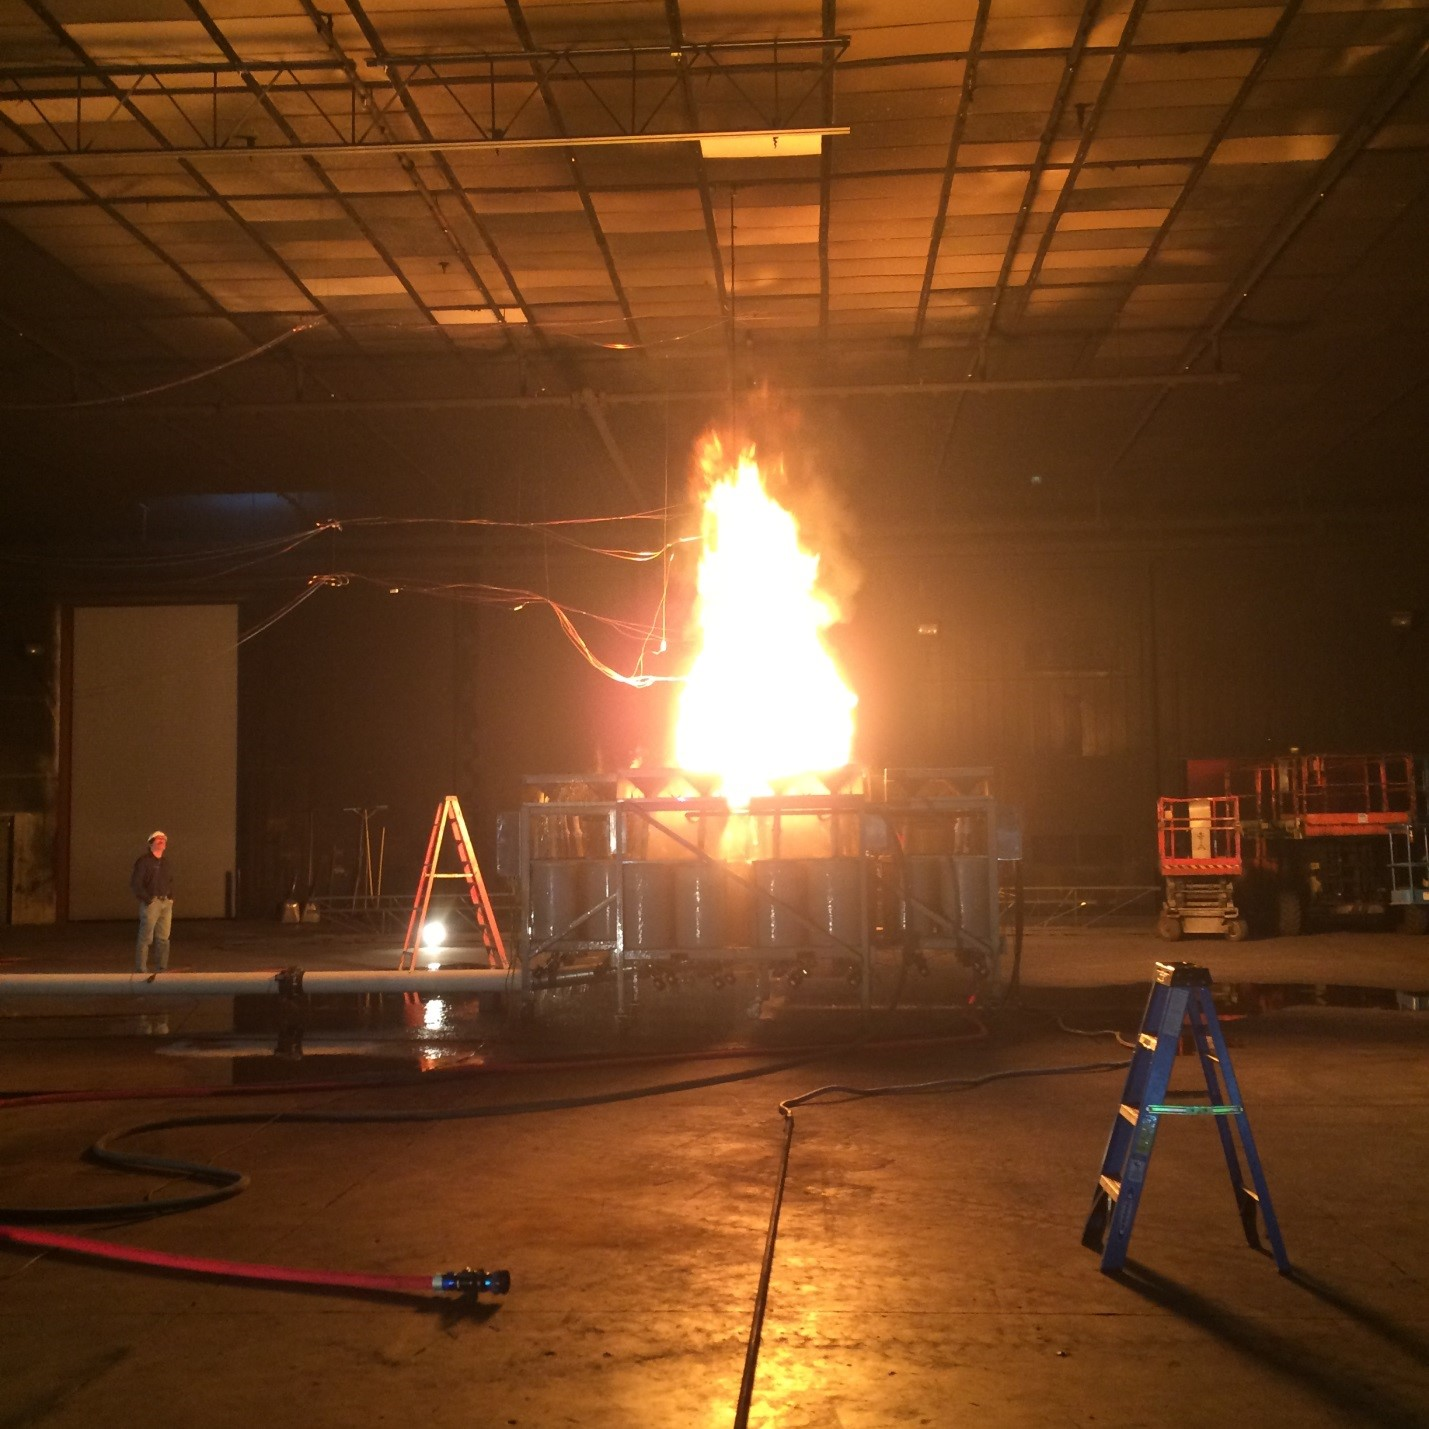
\includegraphics[width=4in]{Figures/Water_Distribution/ADD.jpg}
	\caption{The Actual Delivered Density (ADD) Apparatus Simulating a 2.5 MW Fire}
	\label{fig:ADD_Apparatus_Simulating_fire}
\end{figure}

The concept of the ADD measurement is to simulate the top surface of an array of high storage commodity, and measure the flux of water on this top surface as a result of the spray pattern discharged by one or more sprinklers. The ADD apparatus is designed to perform these measurements while simulating different sized rack storage fires (500~kW to 2.5~MW, in increments of 500~kW). This allows for insight into the effect of a real fire plume on sprinkler spray distribution. Typically, the ADD apparatus is used to simulate commodity underneath one, between two, or between four fire sprinklers. For sprinkler manufacturers, the ADD apparatus can be used as a screening tool for new automatic sprinkler designs. Figure \ref{fig:ADD_Apparatus_Simulating_fire} is a photograph of the UL ADD apparatus in operation.

The UL ADD apparatus is comprised of one main array and two satellite arrays of heavy steel framework. The main array consists of 32 water barrels and water pan collection assemblies while each satellite array contains 8 barrels and collection assemblies. All barrels are of 30-gallon capacity and are connected by a 2-inch diameter hose to a 20 inch by 20 inch inverted square pyramid shaped stainless steel water collection pan above. In total, there are 48 total collection pans/barrels. Differential pressure transducers connect to the bottom of each water collection barrel via flexible tubing. The water level in a given barrel is determined by the head pressure measured by the transducer. The water collection rate is calculated based the change in head pressure over time. As Figure \ref{fig:Top-down schematic view of the ADD apparatus} shows, collection assemblies are arranged into 2x2 arrays so that each group of 4 collection assemblies represents one pallet load of commodity.

\begin{figure}[!ht]
	\centering
	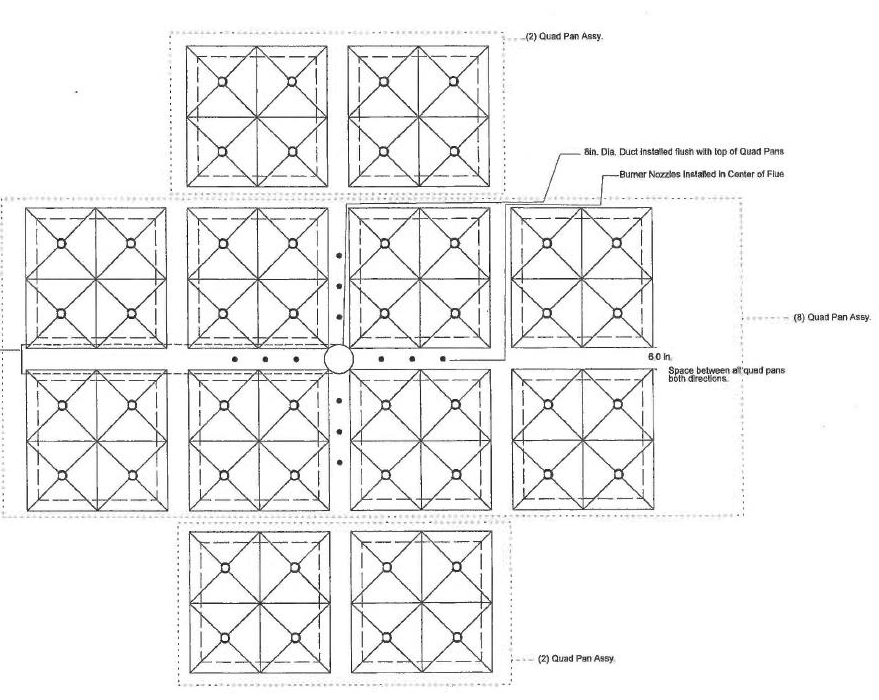
\includegraphics[width=6in]{Figures/Water_Distribution/addschematic.png}
	\caption{Top-down schematic view of the ADD apparatus}
	\label{fig:Top-down schematic view of the ADD apparatus}
\end{figure}

\begin{figure} [H]
	\centering
	\begin{tabular}{c c}
		\subfloat[Collection Barrels]{\includegraphics[height = 2in]{Figures/Water_Distribution/ADD2.jpg}} &
		\subfloat[Collection Pans]{\includegraphics[height = 2in]{Figures/Water_Distribution/ADDbottom3.jpg}} \\
	\end{tabular}
	\caption{ADD Collection Assembly}
	\label{fig:ADD_Collection_Assembly}
\end{figure}

\clearpage
 
Each collection barrel is also connected to a pneumatic drain valve which can be actuated to automatically drain each barrel at the conclusion of each experiment. Figure \ref{fig:Top-down schematic view of the ADD apparatus} also shows flue spaces, as well as an 8 inch duct in the center of the array, which enable the entrainment necessary to simulate a rack-storage fire. A blower supplies air to the center duct to simulate the momentum of the plume of a fire that has reached the top of a rack storage array. Within the center flue spaces of the main array, 12 spray nozzles are angled toward the center to provide the heptane spray used to simulate the commodity fire. Each of the three arrays contains a pipe network and water spray nozzles for cooling the underside of the water collection pans. Cooling is providing during fire simulation to prevent measurement error due to the evaporation of collected water from the hot steel pans, and to prevent absorbed thermal energy from damaging the steel pans.

In December of 2015, data was collected in order to estimate the uncertainty associated with the water distribution experiments performed using the ADD apparatus. Each water collection assembly was filled to capacity while recording pressure transducer measurements as well as data from a calibrated turbine flowmeter (with less than 1~\% measurement uncertainty).
Although the design of each water collection assembly is the same, the measurement performance across the entire apparatus varied in terms of bias and precision. Overall, the water collection assemblies reported volume with a bias of 0.5 gallons less than the volume calculated using the flow meter and with a precision of +/- 2.4 gallons. Using the same data, it is estimated that the real-time (1 Hz) flowrate calculated by the ADD apparatus reported 0.1 gpm less than the turbine flow meter, and with a precision +/- 0.4 gpm.

The recorded data was used to compute a total amount of water in a given bin with the units of gallons.

\clearpage

\section{Test Set Up}

\subsection{Structures}

Part I of the Fire Attack study was comprised of both air entrainment and water distribution testing, each of which involved a different structure.

\subsubsection{Air Entrainment}

The air entrainment testing was conducted at the Delaware County Emergency Services Training Center in Sharon Hill, PA. A two-story purpose built strucutre was constructed several years ago for the use during previous research work conducted by both NIST and UL.

\begin{figure}[!ht]
	\centering
	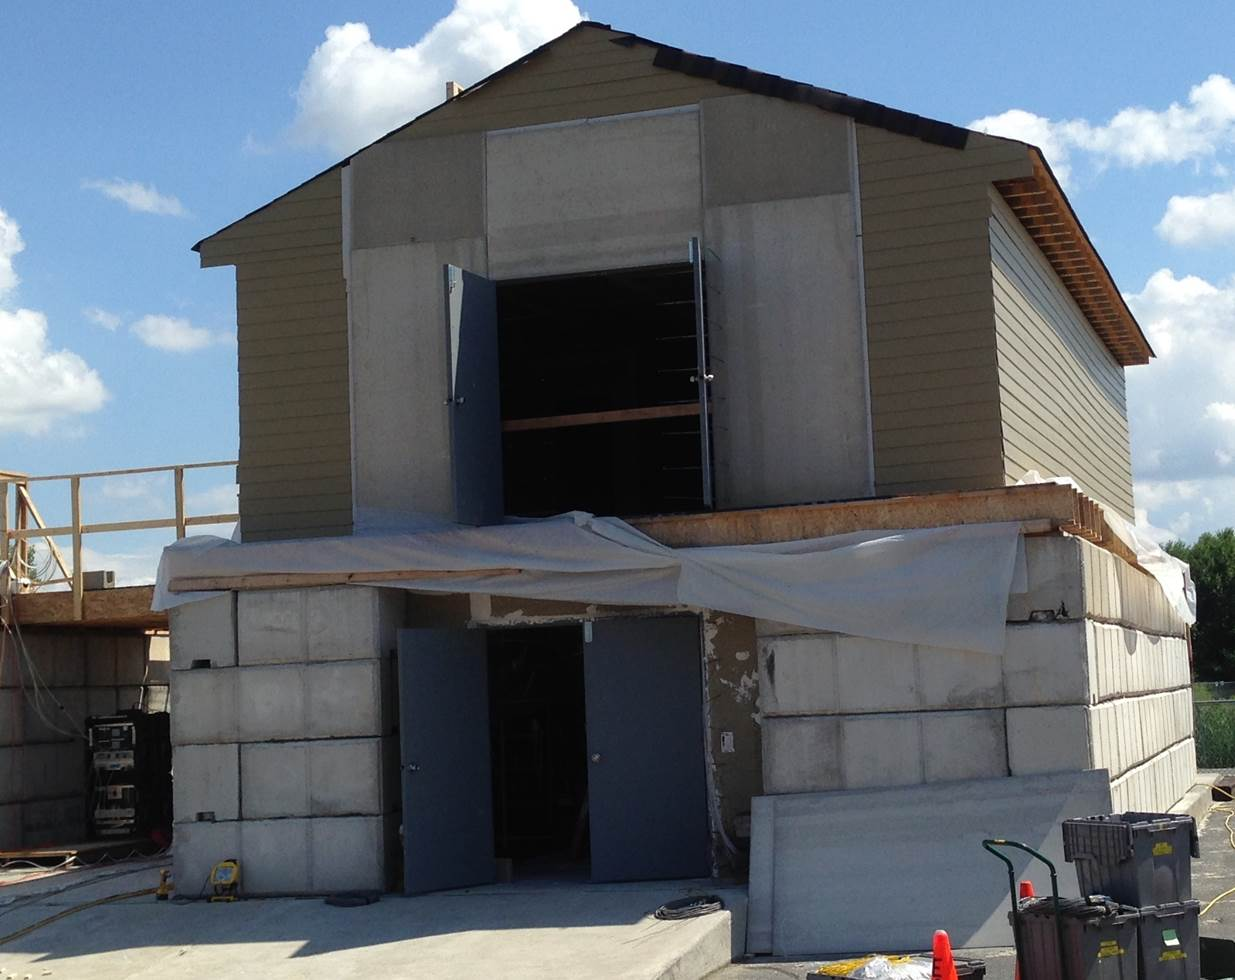
\includegraphics[width=6in]{Figures/Air_Entrainment/DelCo_2story.jpg}
	\caption{Delaware County, PA Fire Test Structure}
	\label{fig:Delaware_County,_PA_Fire_Test_Structure}
\end{figure}

The two-story concrete structure was built on a concrete slab as shown in Fig.~\ref{fig:Delaware_County,_PA_Fire_Test_Structure}. It was designed to simulate a representative residential structure. The outer wall of the structure was composed of interlocking concrete blocks 2~ft wide, 2~ft high and 4~ft long. The interior dimensions of the structure was 20~ft wide, 36~ft long and 8~ft high. The joints and gaps between the blocks were filled with high temperature insulation.

\clearpage

\begin{figure}[!ht]
	\centering
	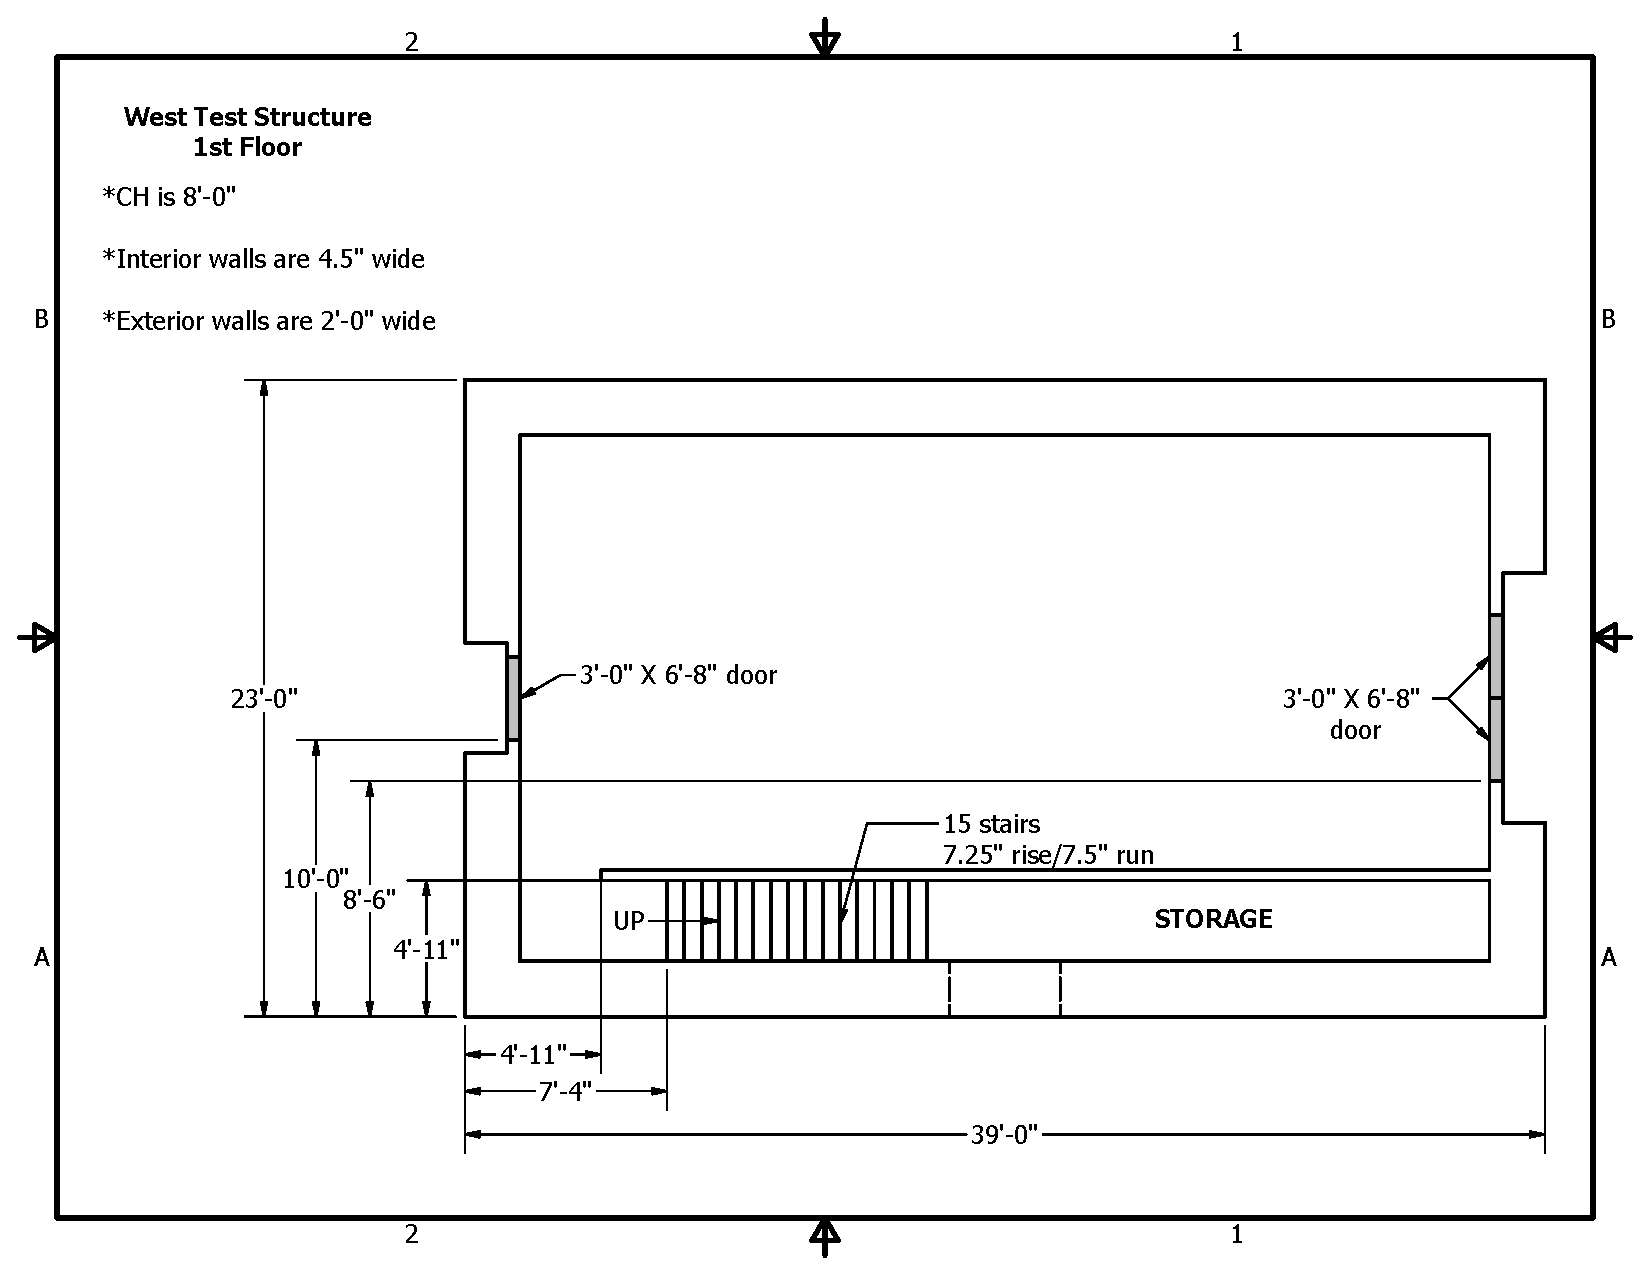
\includegraphics[width=4.5in]{Figures/Air_Entrainment/West_Test_Structure_1st_Floor_original.pdf}
	\caption{Delaware County, PA Fire Test Structure First Floor}
	\label{fig:Delaware_County,_PA_Fire_Test_Structure_First_Floor}
\end{figure}

\begin{figure}[!ht]
	\centering
	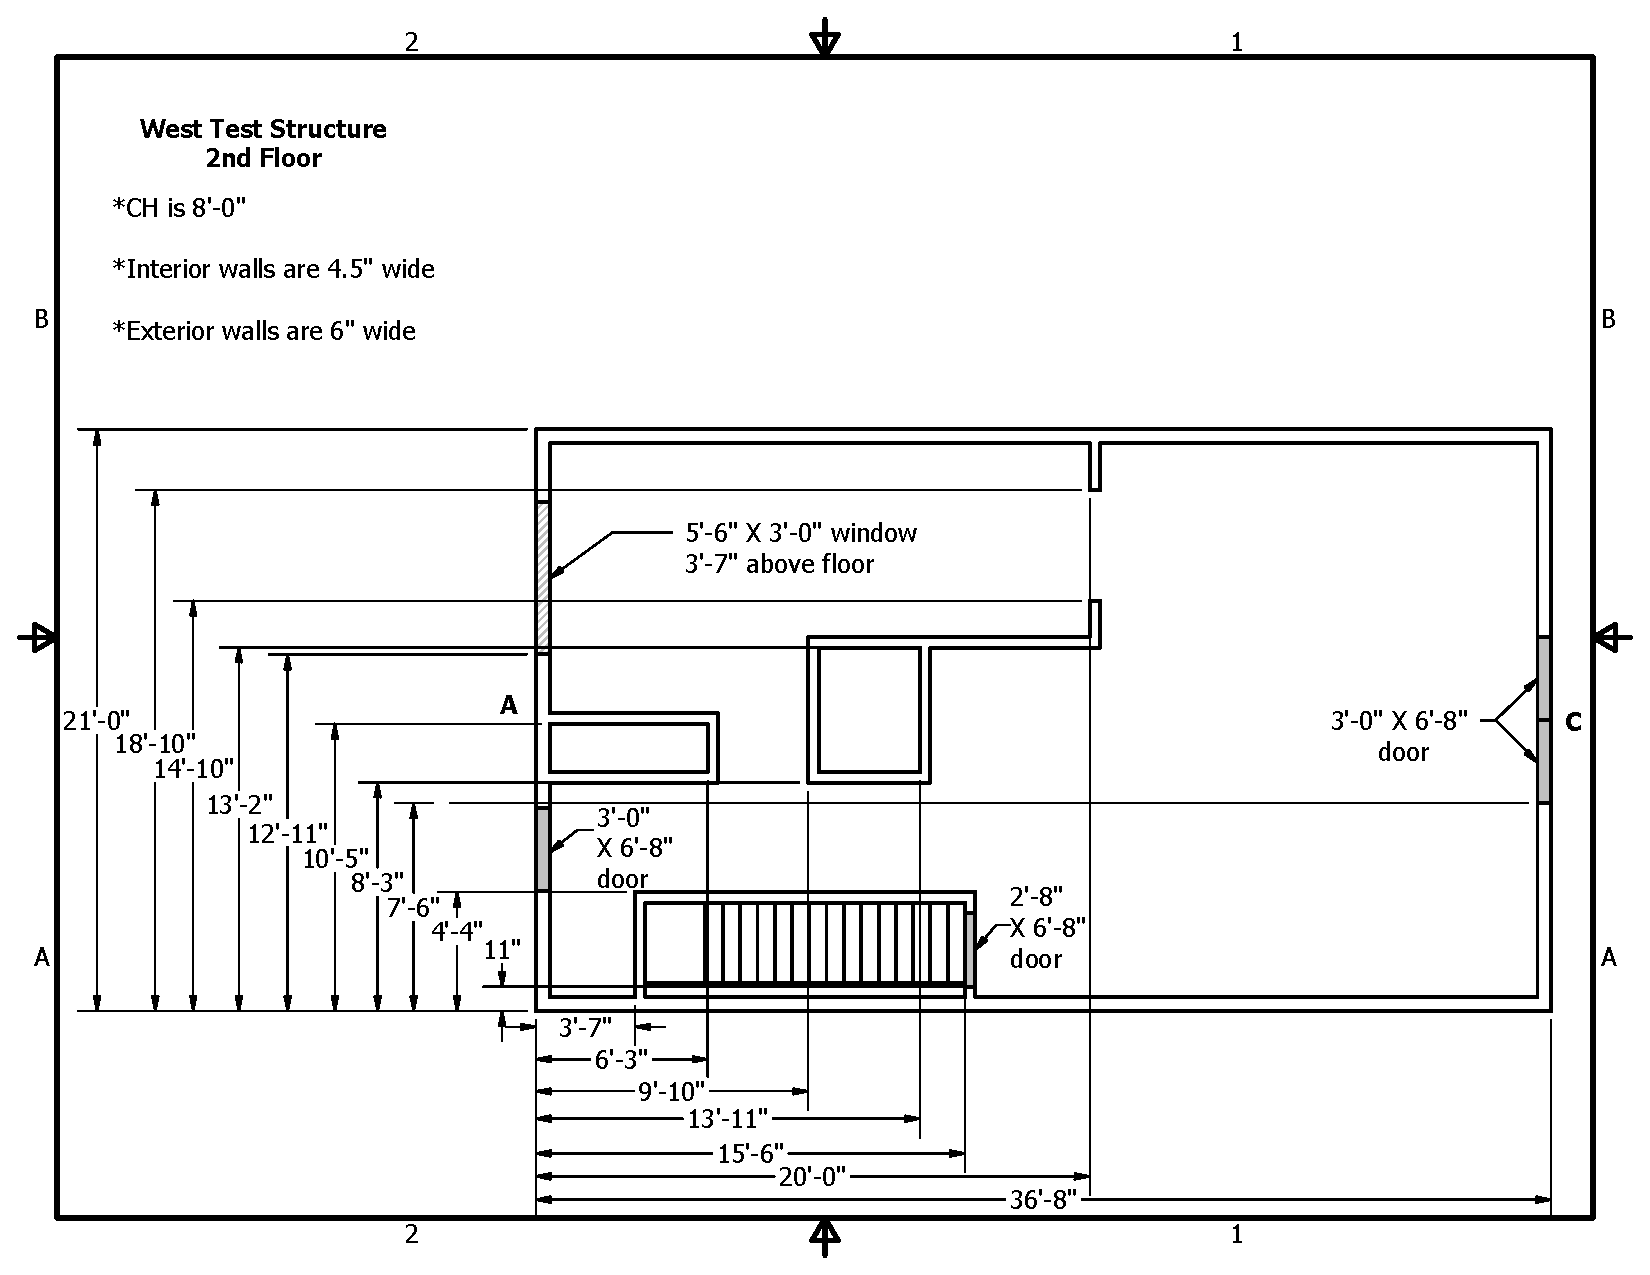
\includegraphics[width=4.5in]{Figures/Air_Entrainment/West_Test_Structure_2nd_Floor.pdf}
	\caption{Delaware County, PA Fire Test Structure Second Floor}
	\label{fig:Delaware_County,_PA_Fire_Test_Structure_Second_Floor}
\end{figure}

\clearpage

The interior walls of the first floor were framed with steel studs set to 16~in. centers and track and were lined with 0.5~in. thick cement board. The walls were composed of 0.63~in. Type X gypsum board. Additionally, the ceiling was composed of two layers of 0.5~in. thick cement board. The first floor ceiling support of the structure was composed of wood truss joist I-beams (TJIs) with a 11.75~in. depth. Each TJI was composed of laminated veneer lumber flanges with a cross section of 1.13~in. x 1.75~in. and an 0.43~in. thick oriented strand board web. Tongue and groove oriented strand board of 0.72~in. thickness was screwed to the top of the TJIs. The second floor of the two story structure was built on the wood ceiling support described above and was connected to the first floor by a stairwell. The walls of the second floor were wood frame with nominal 2~in. by 4~in. studs set to 16~in. centers. The interior walls were protected by 0.63~in. fire rated gypsum board, 0.63~in. durarock board, and a second layer of 0.63~in. fire rated gypsum board. The exterior walls were protected with 0.44~in oriented strand board and 0.31~in. fiber cement lap siding.

The interior layout of the structure can be seen in the dimensioned floor plans above. The interior dimensions of the first and second floors of the structure were 19~ft by 35.1~ft and 20~ft by 35.8~ft, respectively. The stairs connecting the two floors of the structure started 5.3~ft off the South wall with a width of 4~ft off the East wall and contained a 7.25~in rise and 7.5~in run. The exterior doorways of each structure and the stairwell doorway on the second level of the structure all contained steel doors that were opened or closed at certain instances during tests to change the ventilation configuration within the structure. All other doorways in the structures did not contain a door. If it was determined that these doors needed closed during a test, a sheet of either gypsum board or oriented strand board was used to cover the opening and remainded as such until the conclusion of the given test.

\clearpage

\subsubsection{Water Distribution}

Testing for the water distribution experiments was conducted at the UL - Headquarters in Northbrook, IL. A purpose built compartment with a small attached hallway and moveable staircase was constructed to sit atop the ADD apparatus.

\begin{figure}[!ht]
	\centering
	\includegraphics[width=4in]{Figures/Water_Distribution/Building.jpg}
	\caption{Water Distribution Test Structure and ADD Apparatus}
	\label{fig:Water_Distribution_Test_Structure_and_ADD_Apparatus}
\end{figure}

The elevated compartment was build on an existing concrete slab located in one of the rooms within the UL large fire lab. It was designed to simulate a room of size commonly found in residential structures. The size and orientation of the ADD apparatus dictated the overall size of the compartment which measured 15~ft 4~in. by 10~ft 5~in. finished interior dimensions. The compartment was wood frame construction with 2~in. by 4~in. studs and track set to 16~in. centers with a interior height measuring 8~ft 1 1/8~in. rough. The walls and ceiling were lined with 1/2~in. durarock cement board atop 1/2~in. plywood. The ceiling joists were 2~in. by 6~in. set to 16~in. on center. 

\begin{figure}[!ht]
	\centering
	\includegraphics[width=4in]{Figures/Water_Distribution/floor3.jpg}
	\caption{ADD Interior Layout with Flashing}
	\label{fig:ADD_Flashing}
\end{figure}

\clearpage

There was no floor constructed in the compartment as the top of the ADD aparatus served as such. The gaps between the collection bins were covered by flashing which was folded to divert the water evenly in each bin to ensure adequate distribution results. The gaps between the outer collection bins and the walls of the structure were also covered with flashing to ensure all water directed into the structure was collected in the appropriate bins. The interior layout of the structure and use of flashing can be seen in Figure \ref{fig:ADD_Flashing}. 

The compartment featured two ventilation openings, one doorway measuring 3~ft by 6~ft 8~in. which opens to the interior hallway, and one window measuring 2~ft by 4~ft which opens to the exterior of the compartment. A moveable staircase and landing was constructed to provide access to either the interior hallway of the compartment or provide a simulation of a first floor exterior attack. The dimensions of the both the staircase and overall compartment can be seen in the dimensioned drawings below.

\begin{figure}[!ht]
	\centering
	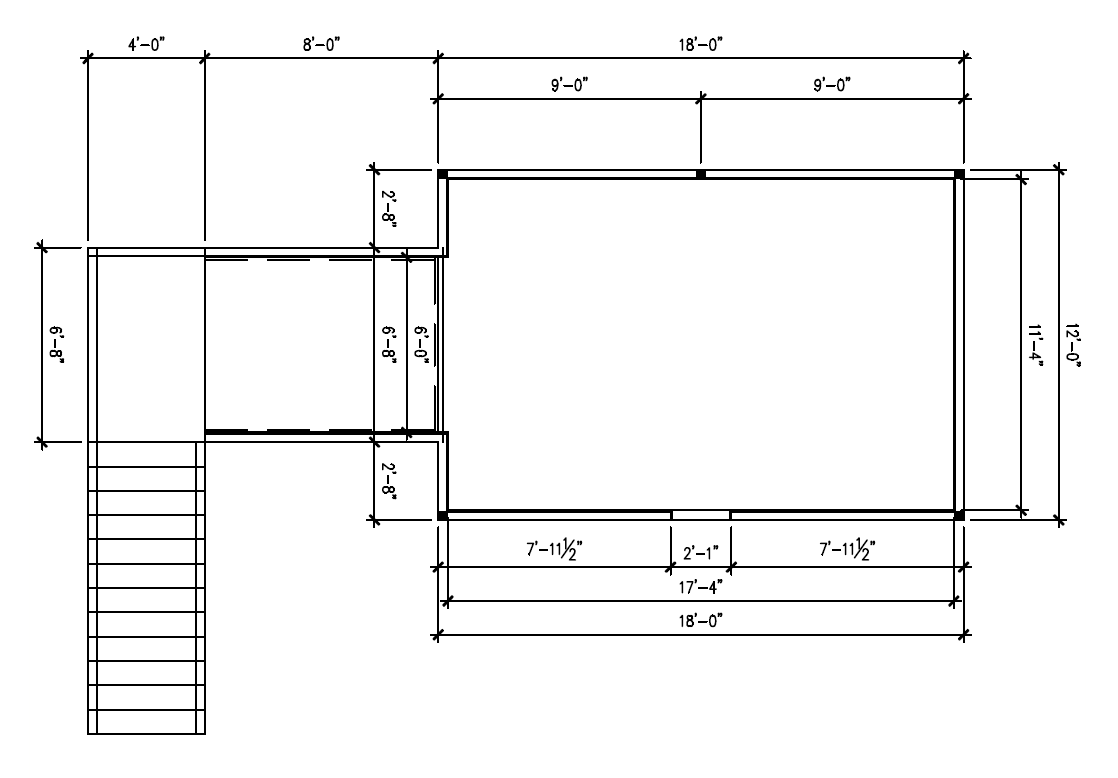
\includegraphics[width=5.5in]{Figures/Water_Distribution/ADDtopviewprint.png}
	\caption{ADD Top View}
	\label{fig:ADD_Top_View}
\end{figure}

\clearpage

\begin{figure}[!ht]
	\centering
	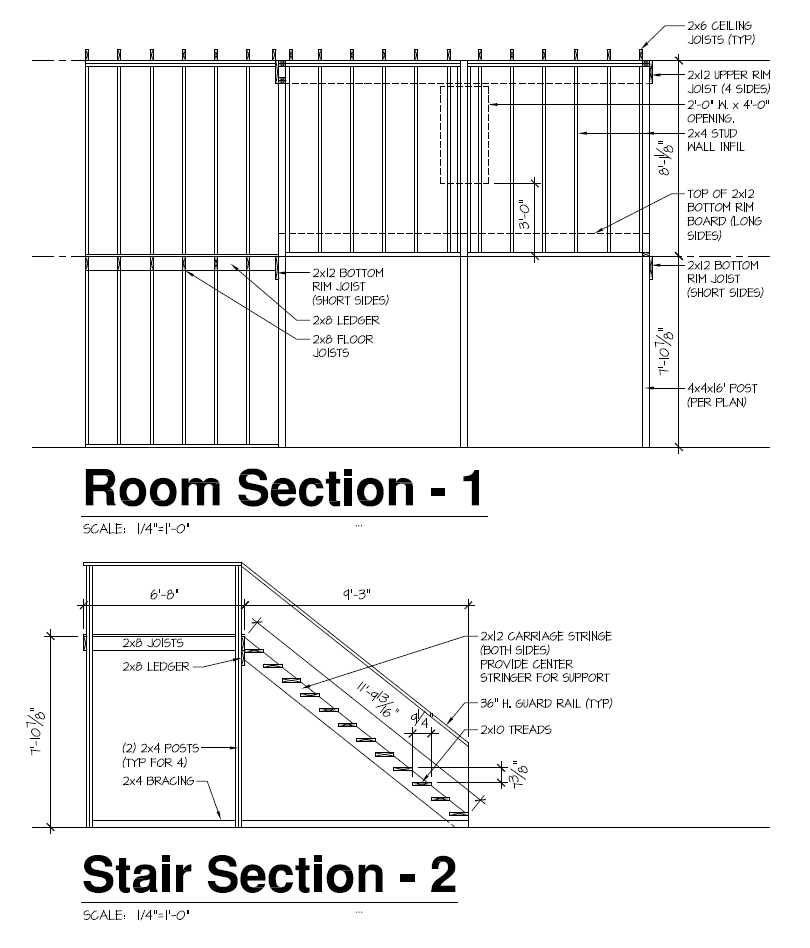
\includegraphics[width=5.5in]{Figures/Water_Distribution/ADDsideviewprint.png}
	\caption{ADD Side View}
	\label{fig:ADD_Side_View}
\end{figure}

\clearpage

\subsection{Measurement Locations}

In order to collect the data needed for this analysis, sensors were installed and measurements were recorded throughout each structure. The measurement locations varied dependent on the structure and desired information.

\subsubsection{Air Entrainment}

When examining the amount of air entrainment in nozzles and caused by variations in hose stream application, several challenges arose in determining the location to measure the gas velocity in the structure. Because the experiments were conducted in an outdoor fixture, considering environmental factors such as wind was critical; especially when quantifying the amount of air moved by nozzles and hose streams. Additionally, the instrumentation used in data collection requires a dry environment to maintain the smallest level of uncertainty and remain operational. In order to combat these challenges, it was determined that the best way to acquire flow data would be to utilize the structure in such a way that there would be an inlet for replacement air, a measurement location, and an exhaust for both the hose streams and air moved. 

\begin{figure}[!ht]
	\centering
	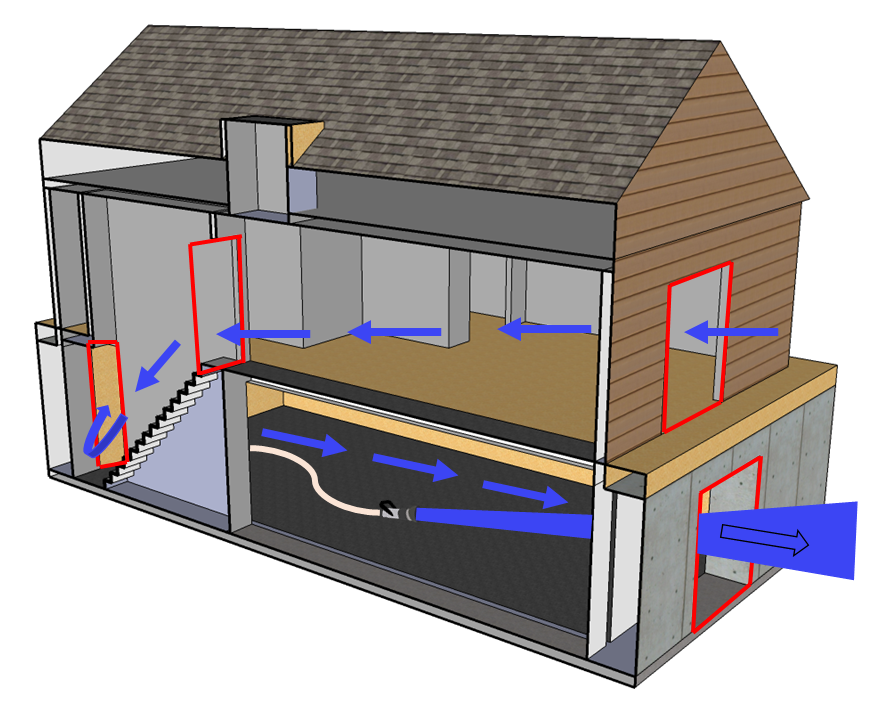
\includegraphics[width=6in]{Figures/Air_Entrainment/Airflow_Layout.png}
	\caption{Air Entrainment Flowpath}
	\label{fig:Air_Entrainment_Flowpath}
\end{figure}

By placing the inlet and exhaust on the same side of the building, we can ensure that any presence of wind does not affect the pressure or air flow within the building. Therefore, the interior environment was consistent throughout the flow path (Figure \ref{fig:Air_Entrainment_Flowpath}) as to not affect the measurements taken. The measurement location was placed in the inlet portion of the flow path in order to keep the instrumentation dry and out of the reach of a hose stream. With the exception of the predetermined inlet and outlet, the remainder of the ventilation openings in the structure remained closed throughout the duration of testing. This ensures that the air entrained by the nozzle is drawn from the inlet location and passes through the measurement location seen in Figure \ref{fig:Measurement_Location_Second_Floor}.

\clearpage

\begin{figure}[!ht]
	\centering
	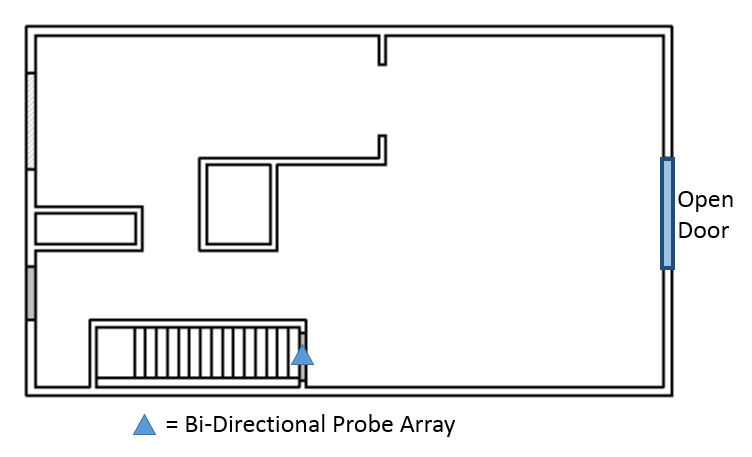
\includegraphics[width=4in]{Figures/Air_Entrainment/Measurement_Locations_Secondfloor.png}
	\caption{Measurement Location (Second Floor)}
	\label{fig:Measurement_Location_Second_Floor}
\end{figure}

\subsubsection{Water Distribution}

The Actual Delivered Density apparatus, described above, was utilized to measure the amount and dsitribution of water flowed into the compartment constructed specifically for this testing. By placing the ADD apparatus beneath the compartment, all of the water flowed was collected and measured. The collection bins were numbered according to their location within the apparatus which allowed a 3D map of the water flow to show the distribution.

\begin{figure}[!ht]
	\centering
	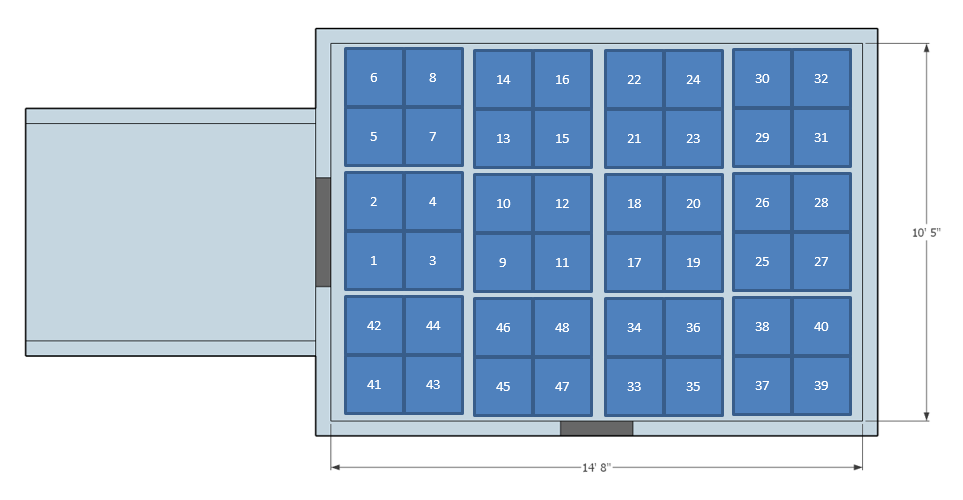
\includegraphics[width=6in]{Figures/Water_Distribution/Measurement_Locations_BinNumbers.png}
	\caption{Bin Numbers and Locations}
	\label{fig:Bin Numbers and Locations}
\end{figure}

\clearpage

\subsection{Equipment Utilized}

In order to ensure the data collected and associated results were applicable to the majority of the fire servce, our technical panel was tasked with creating a list of represetative nozzles, specified flows/pressures, and hose line techniques. All of these variables were tested during both the air entrainment and water distribution experiments; however, several other aspects were held constant such as the length of hose used. The nozzles utilized during these experiments can be seen in the table below.

\begin{table}[]
\centering
\begin{tabular}{|llccc|}
\hline
\multicolumn{1}{|l|}{\textbf{Line Size}} & \multicolumn{1}{l|}{\textbf{Nozzle}} & \multicolumn{1}{l|}{\textbf{Tip (in)}} & \multicolumn{1}{l|}{\textbf{Nozzle Pressure (psi)}} & \textbf{Approximate Flow Rate (gpm)} \\ \hline
1 3/4 in. & Smooth Bore & 1 & 50 & 210 \\
 & Smooth Bore & 15/16 & 50 & 180 \\
 & Smooth Bore & 7/8 & 50 & 150 \\
 & Fog &  & 100 & 100 \\
 & Fog &  & 100 & 150 \\
 & Fog &  & 75 & 150 \\
 & Fog &  & 50 & 150 \\ \hline
2 1/2 in. & Smooth Bore & 1 1/8 & 50 & 260 \\
 & Smooth Bore & 1 1/4 & 50 & 320 \\
 & Fog &  & 100 & 250 \\
 & Fog &  & 75 & 250 \\
 & Fog &  & 50 & 250 \\ \hline
Portable Monitor & Smooth Bore & 1 3/8 & 80 & 500 \\
 & Fog &  & 75 & 500 \\ \hline
Master Stream & Smooth Bore & 1 1/2 & 80 & 600 \\
 & Smooth Bore & 1 3/4 & 80 & 800 \\
 & Fog &  & 100 & 500-1000 \\ \hline
\end{tabular}
\caption{Nozzle Selection}
\label{Nozzle Selection}
\end{table}

\clearpage

\section{Air Entrainment Experiments}

The experiments to determine the amount of air entrained by nozzles and hose streams consisted of several test series to gain a wholelistic view of how varying different components, either with the structure or equipment utilized, affected the end result.

% \hl{A discription of the experiments.} Table \ref{table:Air_Entrainment_Experiments} shows the experiments conducted. 

\subsection{Manufacturer Comparison}

\begin{figure}[!ht]
	\centering
	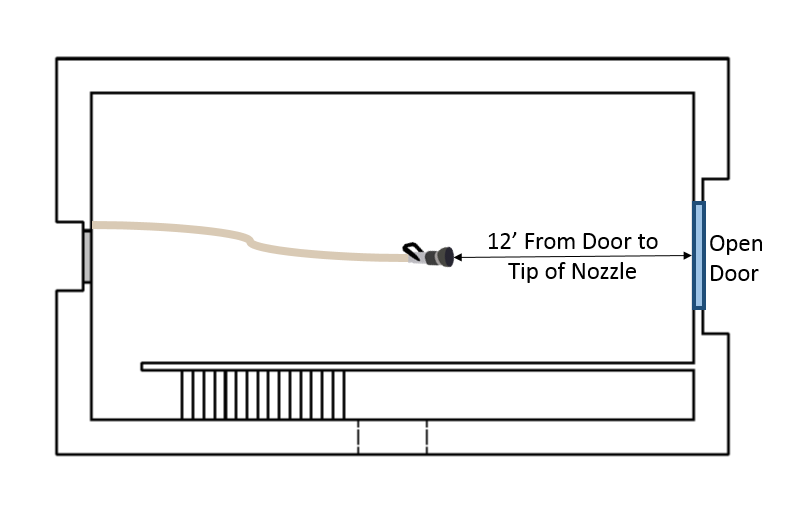
\includegraphics[width=4in]{Figures/Air_Entrainment/Measurement_Locations_Firstfloor.png}
	\caption{Nozzle Position, First Floor, Manufacturer Comparison}
	\label{fig:Nozzle_Position_First_Floor_Manufacturer_Comparison}
\end{figure}

\subsection{Room Configuration}

\begin{figure}[!ht]
	\centering
	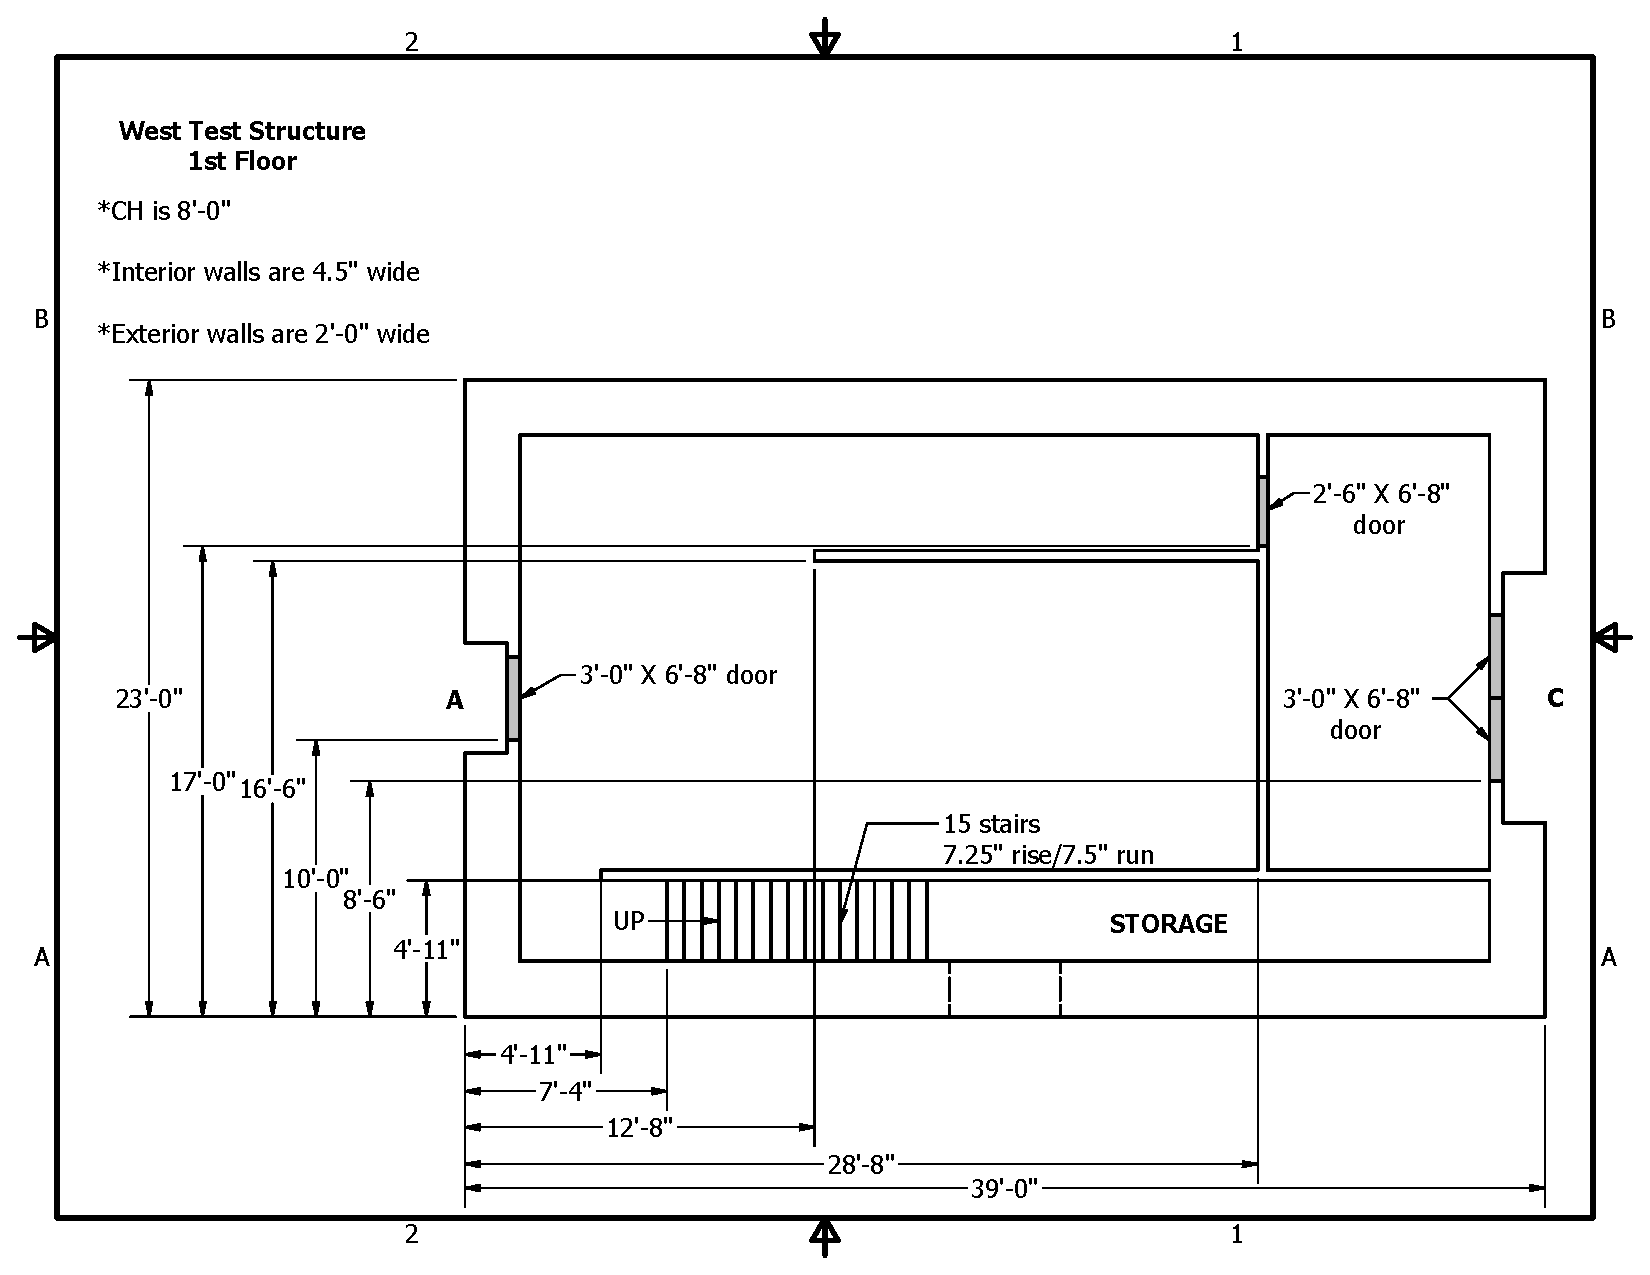
\includegraphics[width=4in]{Figures/Air_Entrainment/West_Test_Structure_1st_Floor.pdf}
	\caption{Room Configuration, First Floor}
	\label{fig:Room Configuration, First Floor}
\end{figure}

\begin{figure}[!ht]
	\centering
	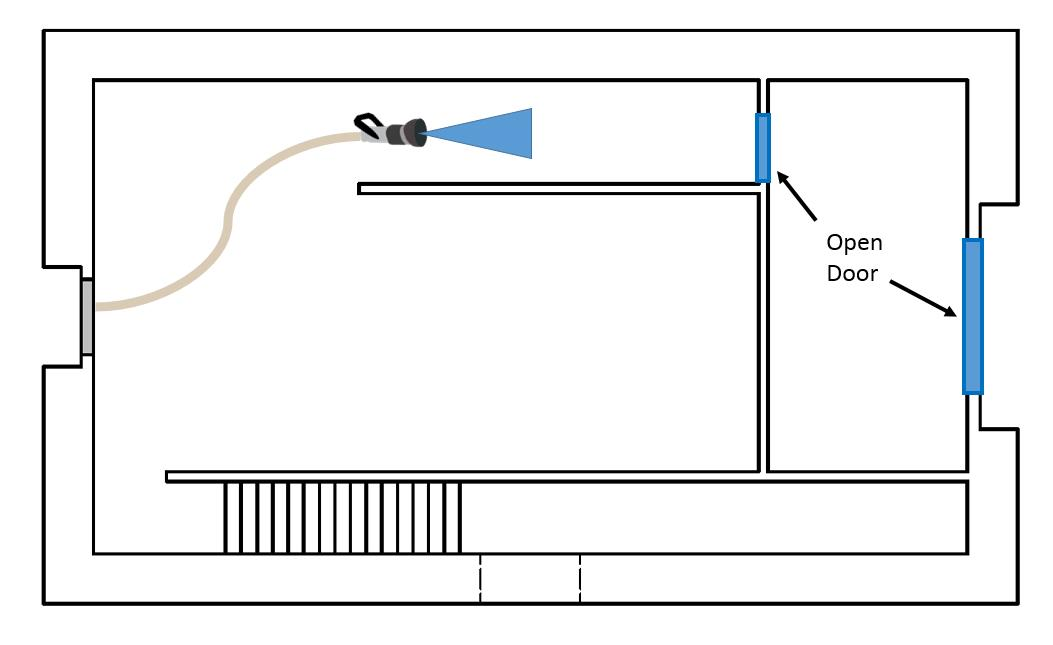
\includegraphics[width=4in]{Figures/Air_Entrainment/Measurement_Location_Room_Configuration.jpg}
	\caption{Nozzle Position, First Floor, Room Configuration}
	\label{fig:Nozzle_Position_First_Floor_Room_Configuration}
\end{figure}

\section{Water Distribution Experiments}

The water distribution experiments incorporated both interior and exterior fire attack utilizing the various nozzles and configurations chosen by the technical panel. 

The interior testing was simulating a fire on the same floor as the attack crew in which the suppression operations were conducted from an adjoining room/hallway. At this position, the nozzle type as well as nozzle direction and application pattern were varied to determine the water distribution within the compartment. The nozzle directions and associated terminology can be seen in Figure \ref{fig:Nozzle_Direction_Interior_Attack}.

\begin{figure}[!ht]
	\centering
	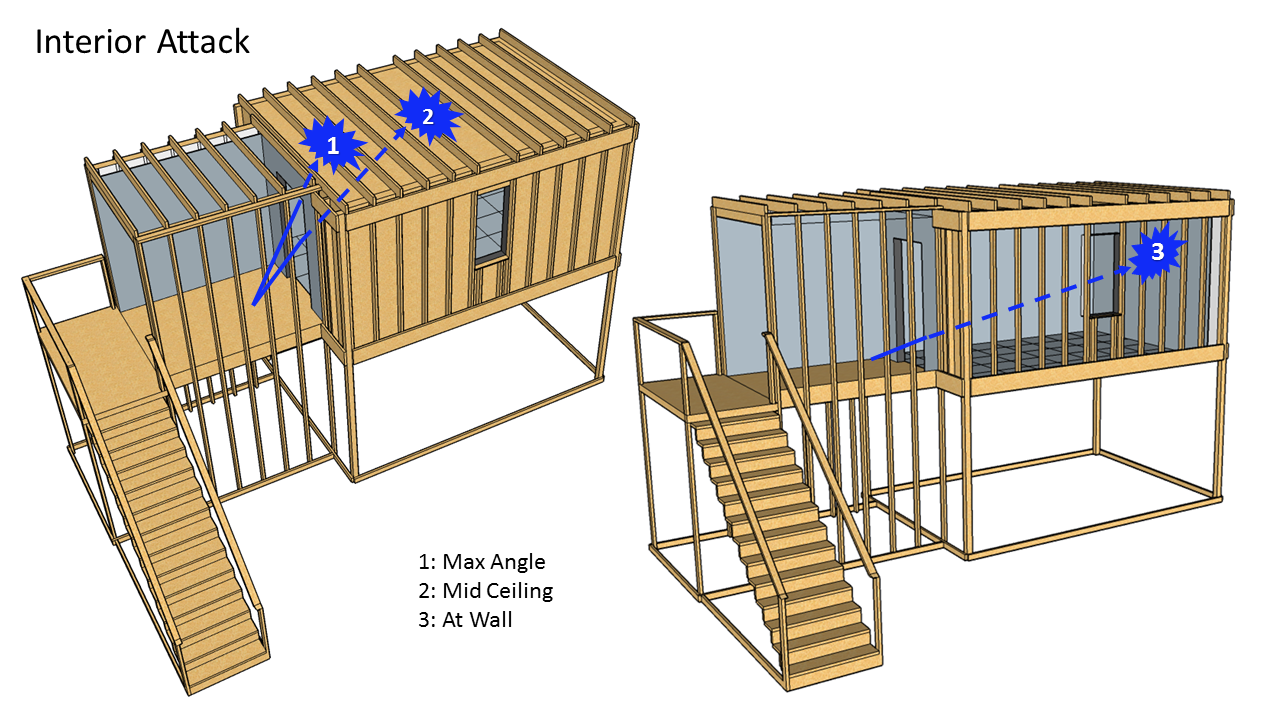
\includegraphics[width=6in]{Figures/Water_Distribution/Nozzle_Position_Int.png}
	\caption{Nozzle Direction, Interior Attack}
	\label{fig:Nozzle_Direction_Interior_Attack}
\end{figure}

\clearpage

\begin{table}[]
\centering
\scalebox{0.7}{
\begin{tabular}{|lccccc|}
\hline
\multicolumn{1}{|c|}{\textbf{Nozzle Position}} & \multicolumn{1}{c|}{\textbf{Nozzle Pattern}} & \multicolumn{1}{c|}{\textbf{Nozzle Direction}} & \multicolumn{1}{c|}{\textbf{Nozzle Type}} & \multicolumn{1}{c|}{\textbf{Nozzle Pressure (psi)}} & \textbf{Flow Rate (gpm)} \\ \hline
At Room Entrance & Fixed & Mid Ceiling & Straight Stream & 100 & 125 \\
At Room Entrance & O & Mid Ceiling & Straight Stream & 100 & 125 \\
At Room Entrance & Z & Mid Ceiling & Straight Stream & 100 & 125 \\
At Room Entrance & T & Mid Ceiling & Straight Stream & 100 & 125 \\
At Room Entrance & Inverted U & Mid Ceiling & Straight Stream & 100 & 125 \\
At Room Entrance & Fixed & Mid Ceiling & Fog & 100 & 125 \\
At Room Entrance & Fixed & Mid Ceiling & Straight Stream & 100 & 150 \\
At Room Entrance & O & Mid Ceiling & Straight Stream & 100 & 150 \\
At Room Entrance & Fixed & Mid Ceiling & Fog & 100 & 150 \\
At Room Entrance & O & Mid Ceiling & Fog & 100 & 150 \\
At Room Entrance & Fixed & Mid Ceiling & Straight Stream & 75 & 150 \\
At Room Entrance & O & Mid Ceiling & Straight Stream & 75 & 150 \\
At Room Entrance & Fixed & Mid Ceiling & Fog & 75 & 150 \\
At Room Entrance & O & Mid Ceiling & Fog & 75 & 150 \\
At Room Entrance & Fixed & Mid Ceiling & Straight Stream & 50 & 150 \\
At Room Entrance & O & Mid Ceiling & Straight Stream & 50 & 150 \\
At Room Entrance & Fixed & Mid Ceiling & Fog & 50 & 150 \\
At Room Entrance & O & Mid Ceiling & Fog & 50 & 150 \\
At Room Entrance & Fixed & At Wall & 15/16 Smooth Bore & 50 & 180 \\
At Room Entrance & O & At Wall & 15/16 Smooth Bore & 50 & 180 \\
At Room Entrance & Fixed & Mid Ceiling & 15/16 Smooth Bore & 50 & 180 \\
At Room Entrance & O & Mid Ceiling & 15/16 Smooth Bore & 50 & 180 \\
At Room Entrance & Fixed & Max Angle & 15/16 Smooth Bore & 50 & 180 \\
At Room Entrance & O & Max Angle & 15/16 Smooth Bore & 50 & 180 \\
At Room Entrance & Fixed & At Wall & Straight Stream & 100 & 150 \\
At Room Entrance & O & At Wall & Straight Stream & 100 & 150 \\
At Room Entrance & Fixed & Max Angle & Straight Stream & 100 & 150 \\
At Room Entrance & O & Max Angle & Straight Stream & 100 & 150 \\
At Room Entrance & O & Mid Ceiling & Fog & 100 & 125 \\
At Hall Entrance & O & At Wall & Straight Stream & 100 & 150 \\
At Hall Entrance & Z & At Wall & Straight Stream & 100 & 150 \\
At Hall Entrance & Pulsing & At Ceiling & Straight Stream & 100 & 150 \\ \hline
\end{tabular}}
\caption{Interior Fire Attack Distribution Experiments}
\label{Interior_Fire_Attack_Distribution_Experiments}
\end{table}

\clearpage

The exterior testing included both an attack from the fire floor as well as the floor below. These were referred to as first floor and second floor attacks for the purpose of this testing. The construction of the compartment featured a moveable staircase to allow for the variation between first floor and second floor suppression. The exterior testing simulated a single room of fire in which a transitional, or exterior attack, was made by suppression crews. As done in the interior testing, both the nozzle type as well as the nozzle direction and application pattern were varied for comparison. The differences in first floor and second floor attacks can been seen in Figures \ref{fig:Nozzle_Direction_Exterior_1st_Floor_Attack} and \ref{fig:Nozzle_Direction_Exterior_2nd_Floor_Attack}.

\begin{figure}[!ht]
	\centering
	\includegraphics[width=6in]{Figures/Water_Distribution/Nozzle_Position_ExtFirstfloor.png}
	\caption{Nozzle Direction, Exterior 1st Floor Attack}
	\label{fig:Nozzle_Direction_Exterior_1st_Floor_Attack}
\end{figure}

\begin{figure}[!ht]
	\centering
	\includegraphics[width=6in]{Figures/Water_Distribution/Nozzle_Position_ExtSecondfloor.png}
	\caption{Nozzle Direction, Exterior 2nd Floor Attack}
	\label{fig:Nozzle_Direction_Exterior_2nd_Floor_Attack}
\end{figure}

\clearpage

\begin{table}[]
\centering
\scalebox{0.7}{
\begin{tabular}{|lccccc|}
\hline
\multicolumn{1}{|c|}{\textbf{Nozzle Position}} & \multicolumn{1}{c|}{\textbf{Nozzle Pattern}} & \multicolumn{1}{c|}{\textbf{Nozzle Direction}} & \multicolumn{1}{c|}{\textbf{Nozzle Type}} & \multicolumn{1}{c|}{\textbf{Nozzle Pressure (psi)}} & \textbf{Flow Rate (gpm)} \\ \hline
Second Floor & Fixed & Max Angle & 15/16 Smooth Bore & 50 & 180 \\
Second Floor & Sweeping & Max Angle & 15/16 Smooth Bore & 50 & 180 \\
Second Floor & Fixed & Mid Ceiling & 15/16 Smooth Bore & 50 & 180 \\
Second Floor & Fixed & Min Angle: Ceiling & 15/16 Smooth Bore & 50 & 180 \\
Second Floor & Fixed & Min Angle: Wall & 15/16 Smooth Bore & 50 & 180 \\
Second Floor & Fixed & Max Angle & 7/8 Smooth Bore & 50 & 150 \\
Second Floor & Fixed & Max Angle & 1 Smooth Bore & 50 & 210 \\
Second Floor & Fixed & Max Angle & Straight Stream & 100 & 150 \\
Second Floor & Sweeping & Max Angle & Straight Stream & 100 & 150 \\
Second Floor & Wide Sweep & Max Angle & Straight Stream & 100 & 150 \\
Second Floor & Fixed & Max Angle: Sill & Straight Stream & 100 & 150 \\
Second Floor & Fixed & Mid Ceiling & Straight Stream & 100 & 150 \\
Second Floor & Fixed & Min Angle: Ceiling & Straight Stream & 100 & 150 \\
Second Floor & Fixed & Min Angle: Wall & Straight Stream & 100 & 150 \\
Second Floor & Fixed & Max Angle & Fog & 100 & 150 \\
Second Floor & Comb (Fixed then O) & Max Angle & Fog & 100 & 150 \\
First Floor & Fixed & Max Angle & 15/16 Smooth Bore & 50 & 180 \\
First Floor & Sweeping & Max Angle & 15/16 Smooth Bore & 50 & 180 \\
First Floor & Fixed & Mid Ceiling & 15/16 Smooth Bore & 50 & 180 \\
First Floor & Fixed & Min Angle: Ceiling & 15/16 Smooth Bore & 50 & 180 \\
First Floor & Fixed & Min Angle: Wall & 15/16 Smooth Bore & 50 & 180 \\
First Floor & Fixed & At Wall & 15/16 Smooth Bore & 50 & 180 \\
First Floor & Fixed & Max Angle & 7/8 Smooth Bore & 50 & 150 \\
First Floor & Fixed & Max Angle & 1 Smooth Bore & 50 & 210 \\
First Floor & Fixed & Max Angle & Straight Stream & 100 & 150 \\
First Floor & Sweeping & Max Angle & Straight Stream & 100 & 150 \\
First Floor & Wide Sweep & Max Angle & Straight Stream & 100 & 150 \\
First Floor & Fixed & Mid Ceiling & Straight Stream & 100 & 150 \\
First Floor & Fixed & Min Angle: Ceiling & Straight Stream & 100 & 150 \\
First Floor & Fixed & Min Angle: Wall & Straight Stream & 100 & 150 \\
First Floor & Fixed & At Wall & Straight Stream & 100 & 150 \\
First Floor & Fixed & Max Angle & Fog & 100 & 150 \\
First Floor & Comb (SS then Fog O) & Max Angle & Fog & 100 & 150 \\
First Floor & Fixed & Max Angle & Straight Stream & 100 & 250 \\
First Floor & Fixed & Min Angle: Ceiling & Straight Stream & 100 & 250 \\
First Floor & Fixed & Max Angle & 1 1/4 Smooth Bore & 50 & 260 \\
First Floor & Fixed & Max Angle & Straight Stream & 100 & 150 \\
First Floor & Fixed & Max Angle & Straight Stream & 100 & 150 \\
First Floor & Fixed & Max Angle & Straight Stream & 100 & 150 \\
First Floor & Fixed & Max Angle & Straight Stream & 100 & 150 \\
First Floor & Fixed & Max Angle & Straight Stream & 100 & 150 \\
First Floor & Fixed & Max Angle & 15/16 Smooth Bore & 50 & 180 \\
First Floor & Fixed & Max Angle & 15/16 Smooth Bore & 30 & 150 \\
First Floor & Fixed & Max Angle & 15/16 Smooth Bore & 15 & 130 \\
First Floor & Fixed & Max Angle & 15/16 Smooth Bore & 10 & 100 \\
First Floor & Fixed & Max Angle & Straight Stream & 50 & 150 \\
First Floor & Fixed & Max Angle & Straight Stream & 75 & 60 \\
First Floor & Fixed & Max Angle & Straight Stream & 50 & 185 \\
First Floor & Fixed & Max Angle & Straight Stream & 25 & 130 \\ \hline
\end{tabular}}
\caption{Exterior Fire Attack Distribution Experiments}
\label{Exterior_Fire_Attack_Distribution_Experiments}
\end{table}

\clearpage

\section{Experiment Analysis}

\subsection{Air Entrainment Analysis}

\vspace*{\baselineskip}
\paragraph{Air entrainment in nozzles is dependent on nozzle type (smooth bore, straight stream, fog) and not nozzle manufacturer.} \mbox{}



\paragraph{Air entrainment in nozzles is dependent on structure geometry and configurations.} \mbox{}



\paragraph{Nozzle application patterns have little effect on overall air entrainment.} \mbox{}



\paragraph{Air entrainment, either into or out of the strucutre, is dependent on the distance of the nozzle to the ventilation opening.} \mbox{}



\vspace*{\baselineskip}

\clearpage

\subsection{Water Distribution Analysis}

The results from the water distribution testing yielded several tactical considerations for suppression operations on the fireground. These are outlined below along with examples from the results. There are several key points to keep in mind when viewing the analysis. 

The experiments conducted for water distribution were approximately 1 minute in length. This was dictated by the size of the collection barrels in the ADD apparatus. Each collection barrel was a total of 30 gallons. At the start of each test, there was a predetermined amount of water in the bottom of the barrel to ensure the sensors were able to record the intial water received during the testing. This `predetermined' amount of water was recorded prior to the start of the test and was subtracted from the final total so that the end results were not affected by the measurement technique. 

Because of these limitations, the results were only plotted to 20 gallons to minimize uncertainty. Additionally, various bins in various tests only received a final total of a couple gallons or less, and thus, appending the charts to 20 gallons, allows the viewer to more easily see these results. Please keep in mind that the intent of the testing was to determine the location of where water is going within the compartment and not necessarily the total quantity of water that reached a given area. As such, focus on the overall distribution and not the amount of water to a given area.

\subsubsection{Repeatability}

It should be noted that several tests were conducted to determine the repeatability of the experiments to ensure accuracy in the results as well as several tests utilizing `live-fire' in order to detemine the applicability of this testing to the remainder of the study.

Four tests utilizing a straight stream nozzle flowing 150~gpm at 100~psi from the exterior first floor position directed into the structure with a maximum angle were conducted to determine the variance in results.

\clearpage

\begin{figure}[ht]
\begin{tabular*}{\textwidth}{lr}
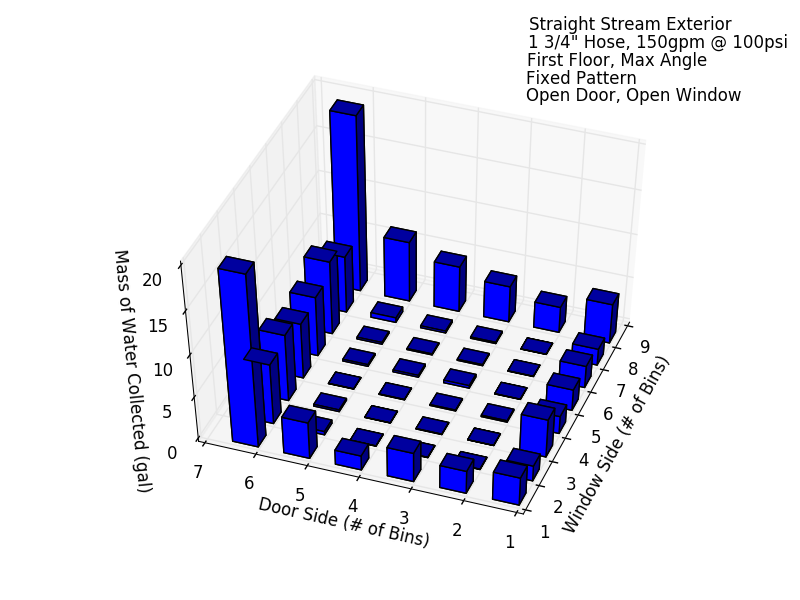
\includegraphics[width=3.2in]{../ADD_Analysis/Figures/15-12-10_082039_Datafile_Straight_Stream_Exterior.png} &
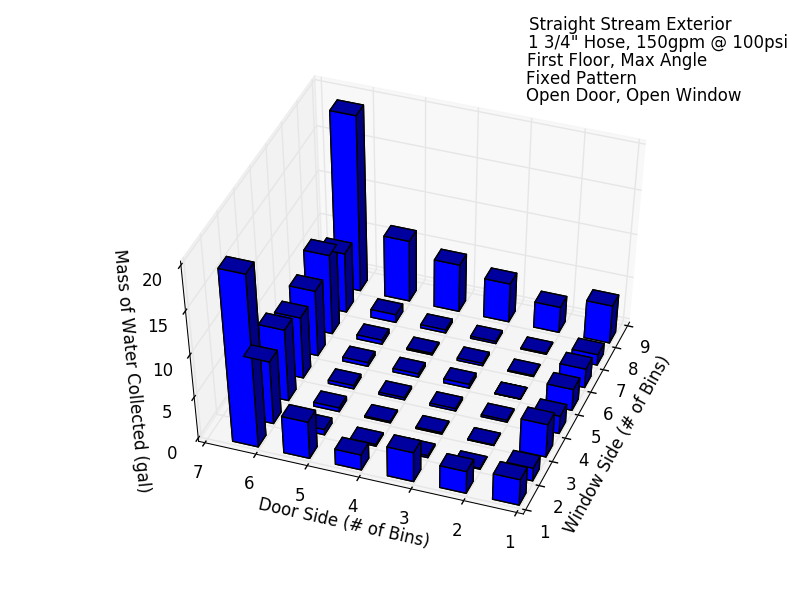
\includegraphics[width=3.2in]{../ADD_Analysis/Figures/15-12-10_082423_Datafile_Straight_Stream_Exterior.png} \\
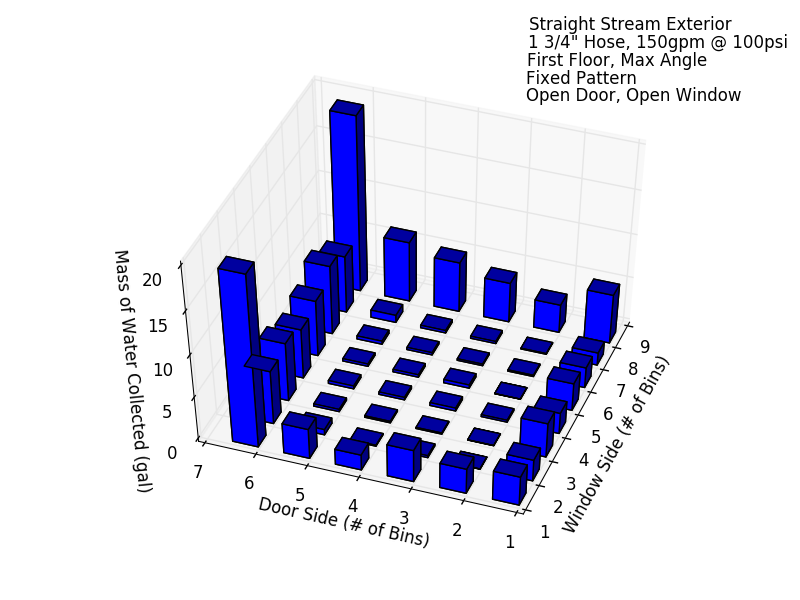
\includegraphics[width=3.2in]{../ADD_Analysis/Figures/15-12-10_083305_Datafile_Straight_Stream_Exterior.png} &
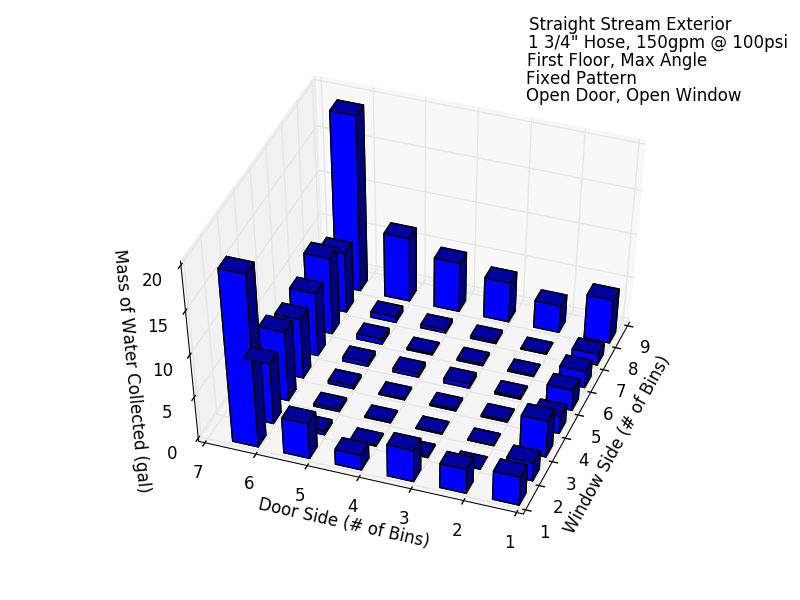
\includegraphics[width=3.2in]{../ADD_Analysis/Figures/15-12-10_083751_Datafile_Straight_Stream_Exterior.png} \\
\end{tabular*}
\caption{Figures showing repeatability in test results.}
\label{fig:Repeatability_Testing}
\end{figure}

\vspace*{\baselineskip}

From these results, it is clear that the differences between the tests were minimal and thus determined that the measurement technique was repeatable.

\clearpage

\subsubsection{Comparison to Fire Testing}

Additionally, two tests were conducted using `live fire' in which two UL 199 standard commodity wooden cribs were placed in the center of the compartment, as shown in Figure \ref{fig:Wood_Crib_Location}, atop a collection pan filled with heptane. The wooden cribs were chosen because of their ability to maintain a near constant burn rate for a period of time. Wooden cribs have been used in the standards testing of sprinklers for many years. The wood cribs were constructed of kiln-dried spruce or fir sticks measuring 1.5~in. high by 1.5~in. wide by 20~in. long. These were fastened together with nails and stacked atop one another to form the overal structure (10 alternating layers, with 5 sticks per layer). The crib measured 20~in. wide by 20~in. deep by 15~in. high and weighed approximately 33~lbs. each. Two cribs were stacked atop one another to ensure the steady burning period of the fire would last for the duration of the experiment. In order to shorten the time to reach the steady burning period and assist in the near uniform ignition of the cribs, 32~oz of Heptane was poured in the pan beneath and ignited with a propane torch.

\begin{figure}[!ht]
	\centering
	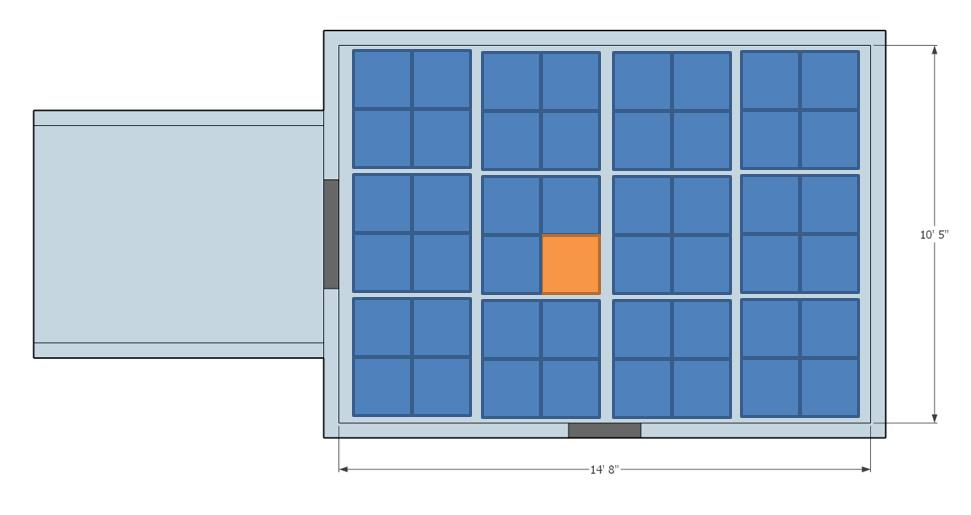
\includegraphics[width=4in]{Figures/Water_Distribution/ADDcriblocation.jpg}
	\caption{Wood Crib Location}
	\label{fig:Wood_Crib_Location}
\end{figure}

\begin{figure} [H]
	\centering
	\begin{tabular}{c c}
		\subfloat[Wooden Cribs]{\includegraphics[height = 2.5in]{Figures/Water_Distribution/WoodCrib2.jpg}} &
		\subfloat[Fire Test]{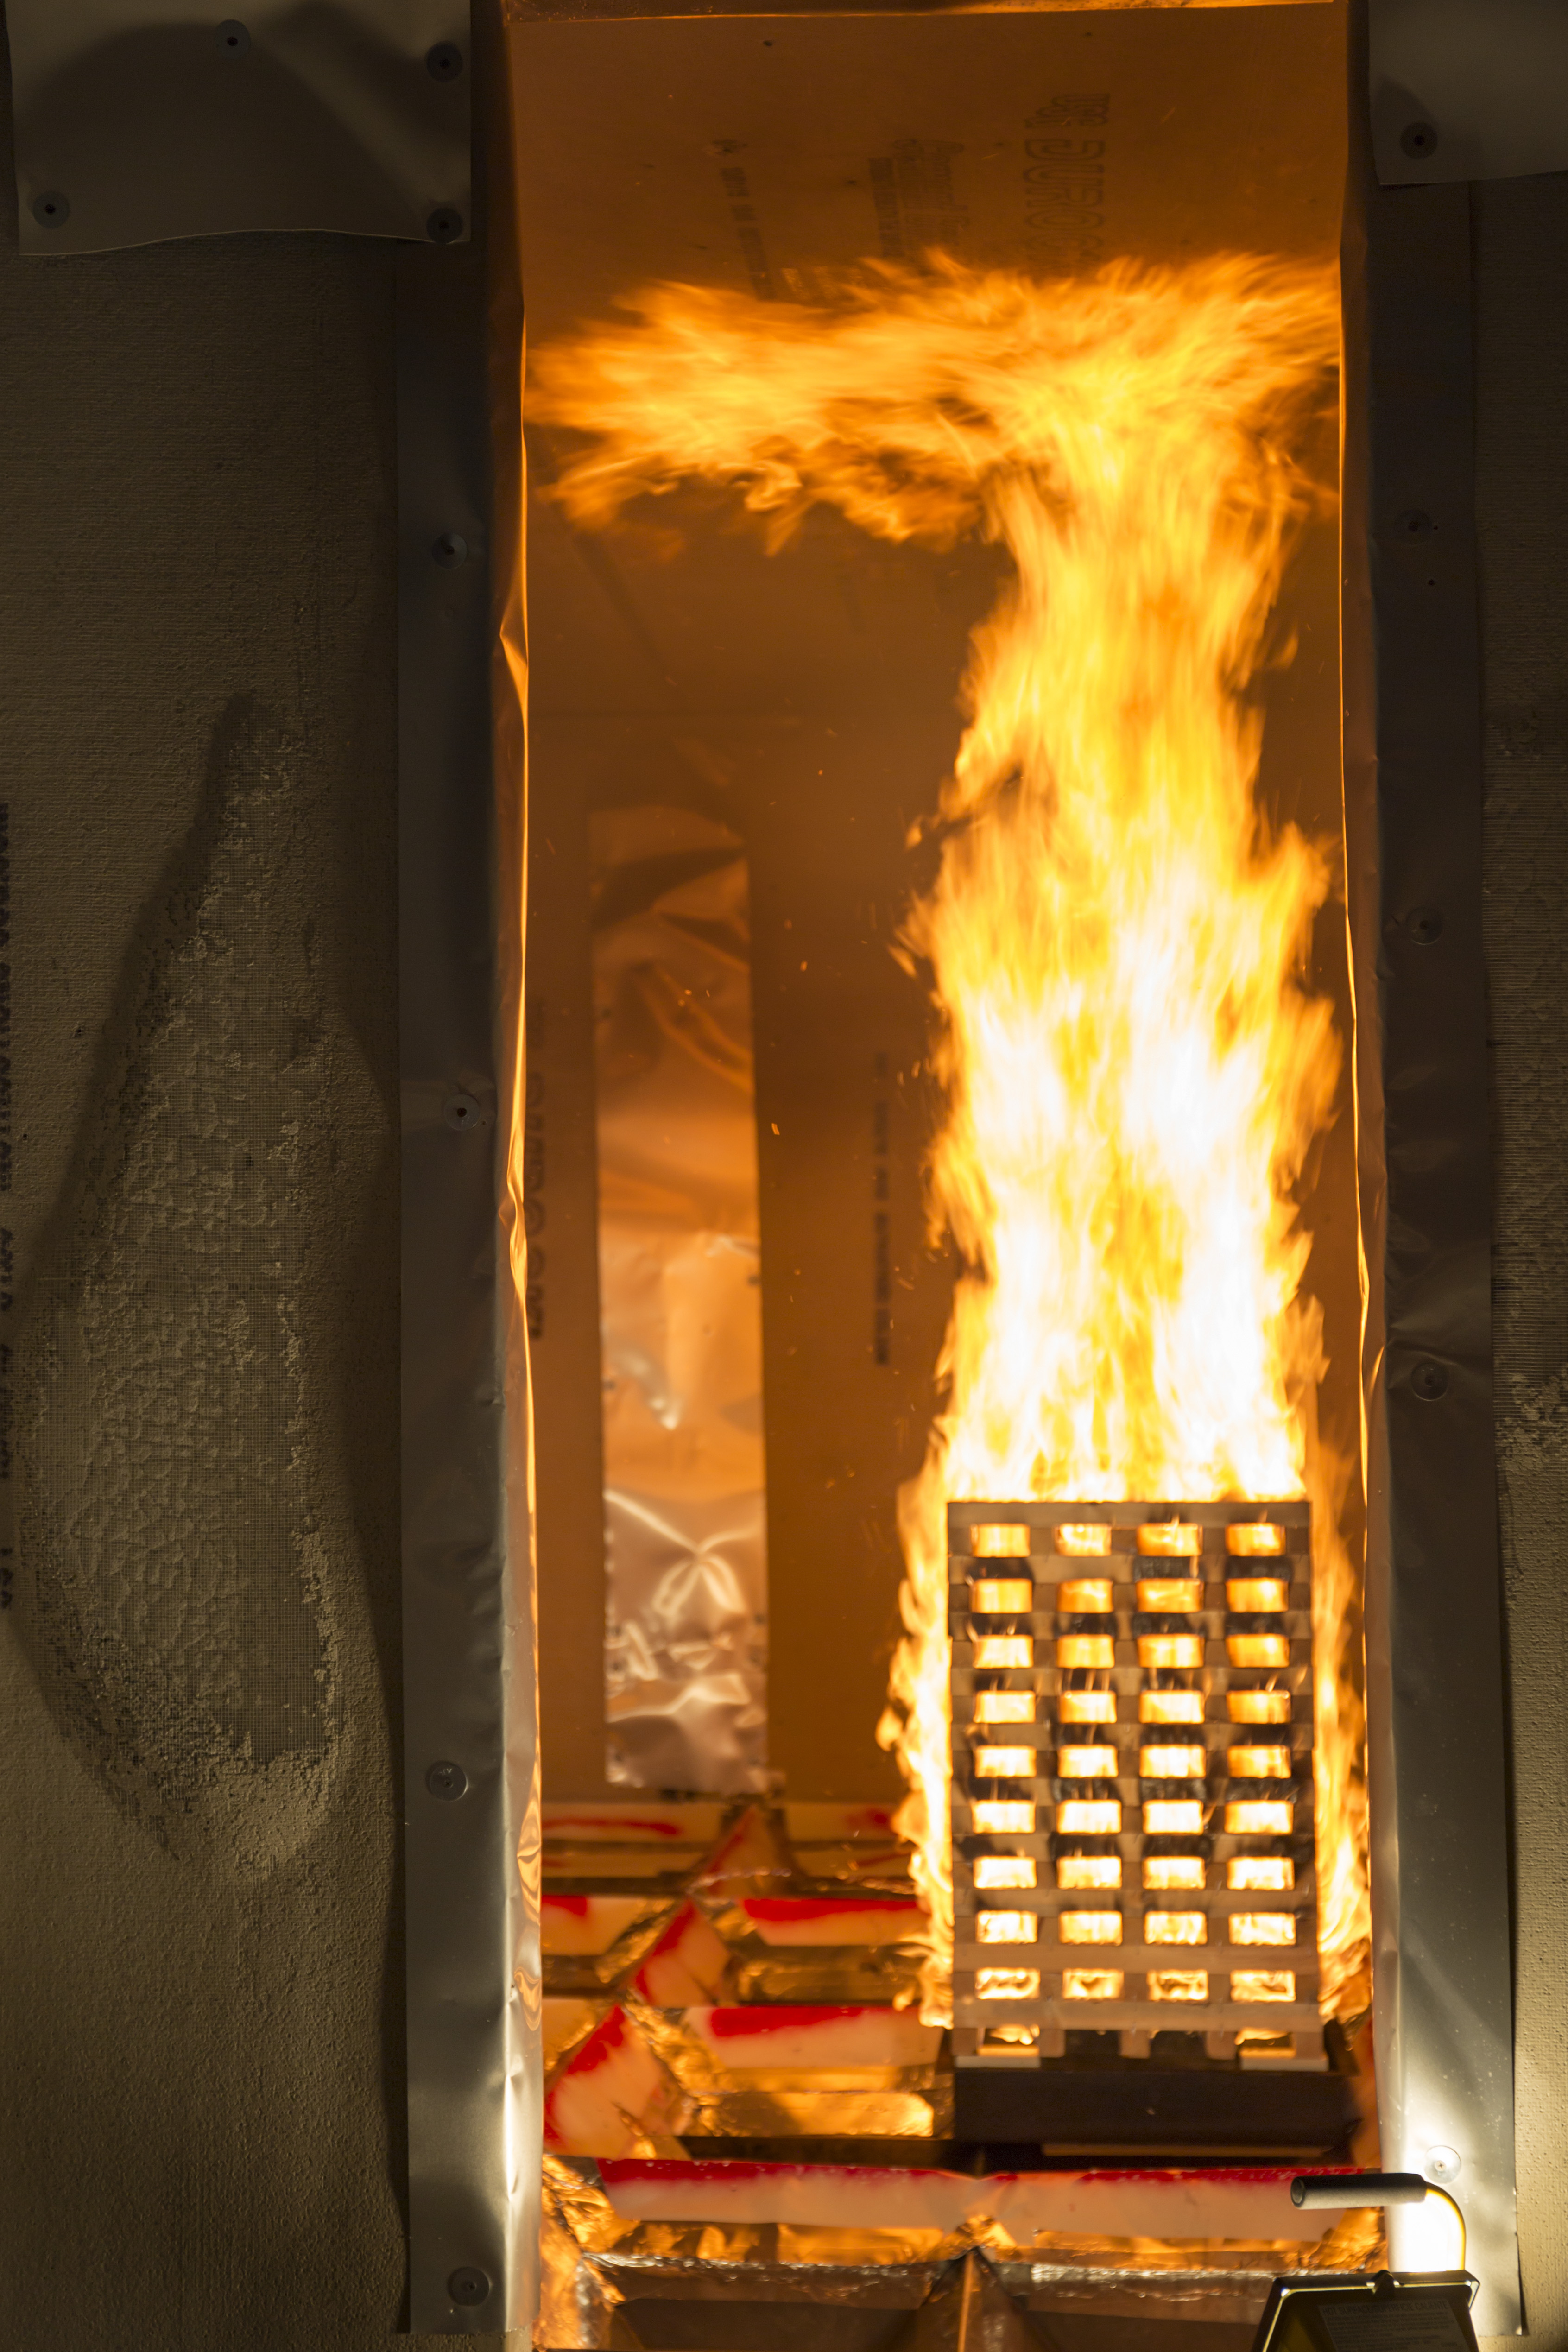
\includegraphics[height = 2.5in]{Figures/Water_Distribution/WoodCribfire3.jpg}} \\
	\end{tabular}
	\caption{ADD Fire Tests}
	\label{fig:ADD_Fire_Tests}
\end{figure}

\clearpage

The results of the two fire tests are shown below as compared to the same tests conducted without `live fire.'

\vspace*{\baselineskip}

\begin{figure}[ht]
\begin{tabular*}{\textwidth}{lr}
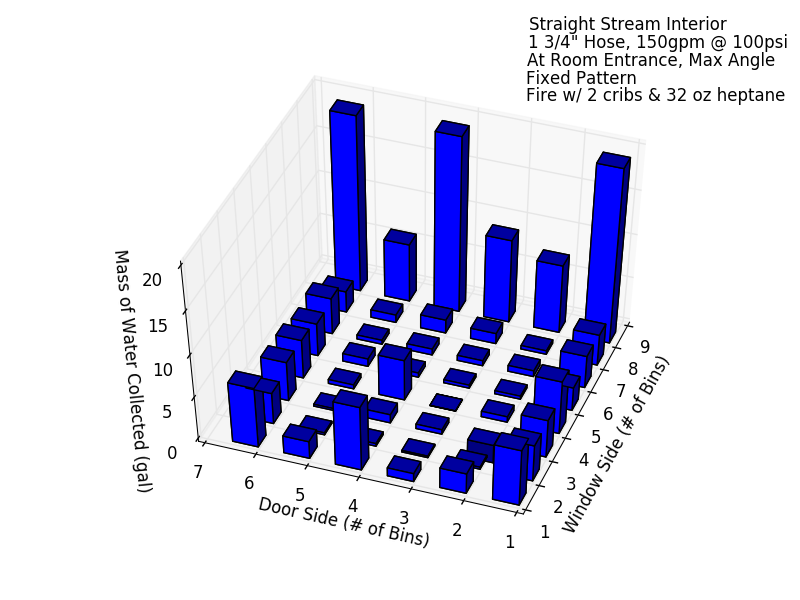
\includegraphics[width=3.2in]{../ADD_Analysis/Figures/15-12-10_132600_Datafile_Straight_Stream_Interior.png} &
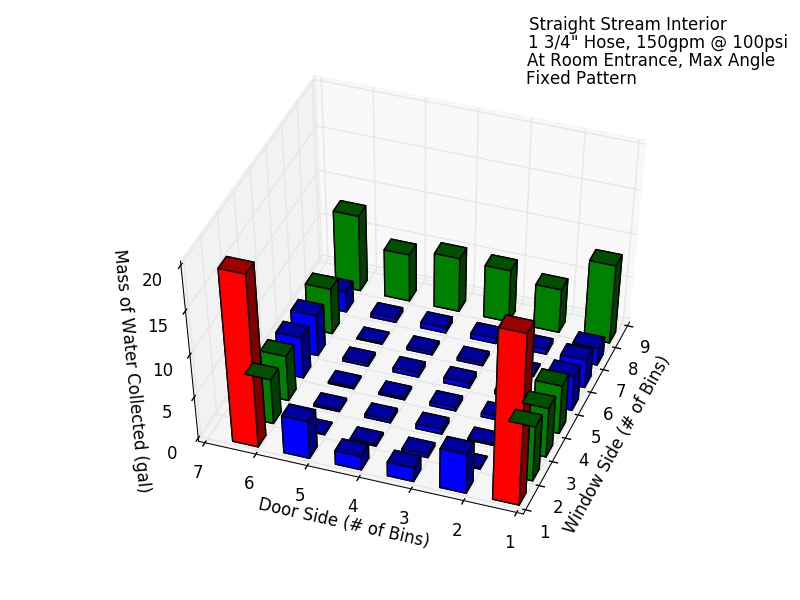
\includegraphics[width=3.2in]{../ADD_Analysis/Figures/15-12-09_152435_Datafile_Straight_Stream_Interior.png} \\
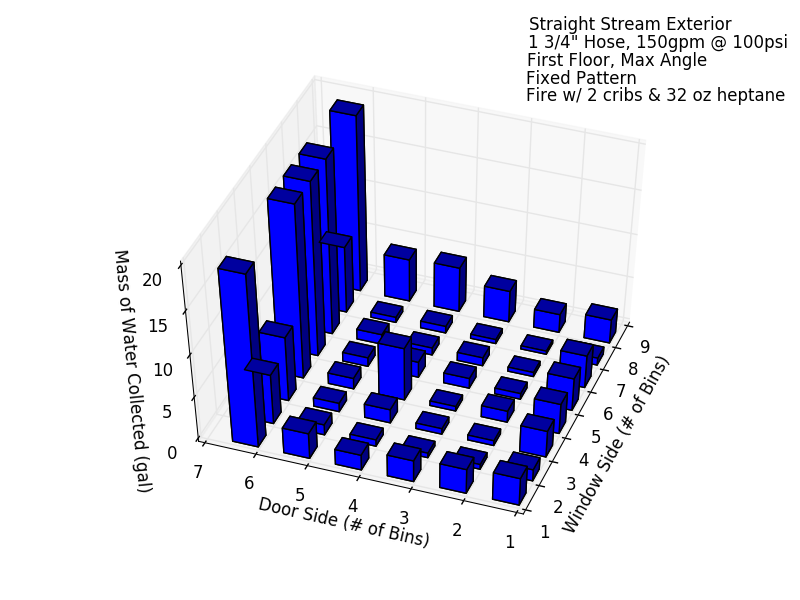
\includegraphics[width=3.2in]{../ADD_Analysis/Figures/15-12-10_122043_Datafile_Straight_Stream_Exterior.png} &
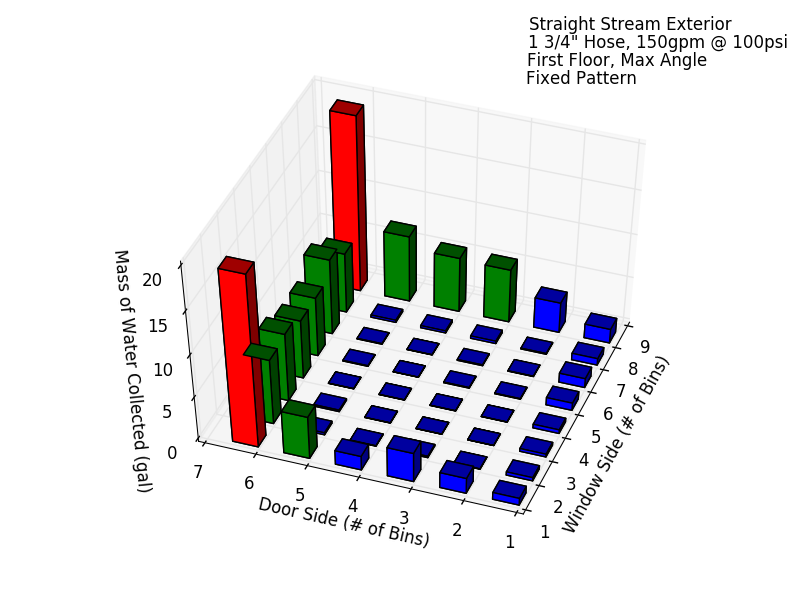
\includegraphics[width=3.2in]{../ADD_Analysis/Figures/15-12-08_113237_Datafile_Straight_Stream_Exterior.png} \\
\end{tabular*}
\caption{`Live fire' comparison results.}
\label{fig:Live_Fire_Comparison}
\end{figure}

From these results, it was determined that the distributions were similar with or without the presence of fire. The small differences can be attributed to several aspects of the testing, including:

\begin{itemize}
	\item As the water passes into the heated compartment and contacts the hot gas layer, some of the water is converted to steam as it heats up and thus the total quantity of water making it into the bins will be slightly smaller in the fire tests.
	\item The collection bins immediately adjacent to the bin where the wooden cribs were placed showed a higher amount of water collected in the fire tests when compared to those without fire. This is attributed to some of the water deflecting off of the crib and falling into the bins surrounding the crib.
\end{itemize}

% If the attack is made from either the interior or exterior of the structure and the stream is directed at the ceiling, the majority of the water `rides' down the opposite wall from the nozzle location, with little to no water making it into the center of the compartment.

\clearpage

\paragraph{Water distribution is dependent on nozzle type (smooth bore, straight stream, fog).} \mbox{}

% ------------------------------------------------------------------------------------
% Interior
% ------------------------------------------------------------------------------------

% Interior (at room entrance, fixed pattern, set flow/pressure)
% 	SS (150 @ 50), Fog (150 @ 50), 15/16 SB (180 @ 50)
% 	15-12-09_121955_Datafile, 15-12-09_123142_Datafile, 15-12-09_144839_Datafile

\begin{figure}[ht]
\begin{tabular*}{\textwidth}{lr}
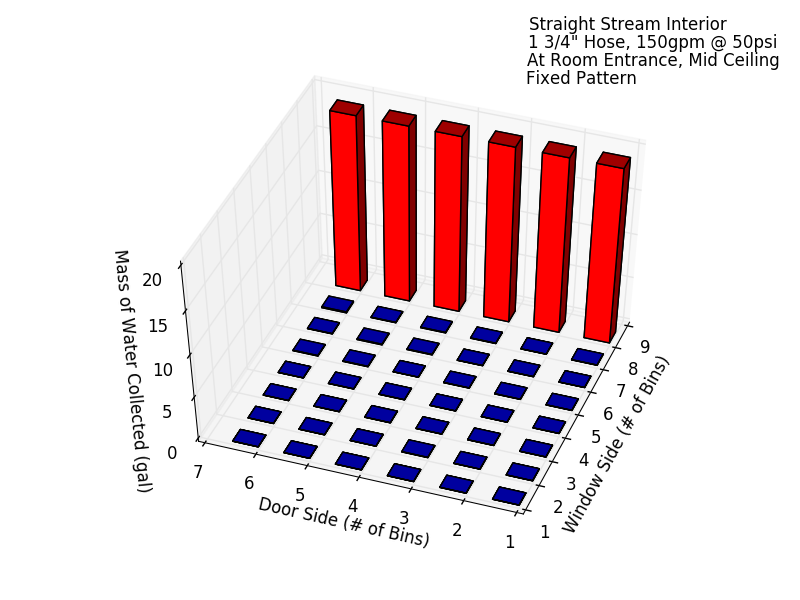
\includegraphics[width=3.2in]{../ADD_Analysis/Figures/15-12-09_121955_Datafile_Straight_Stream_Interior.png} &
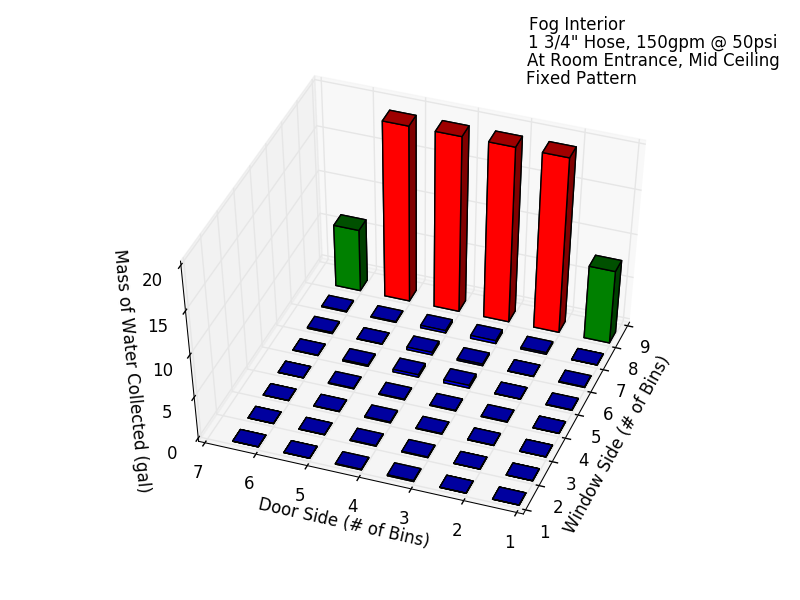
\includegraphics[width=3.2in]{../ADD_Analysis/Figures/15-12-09_123142_Datafile_Fog_Interior.png} \\
\end{tabular*}
\centering
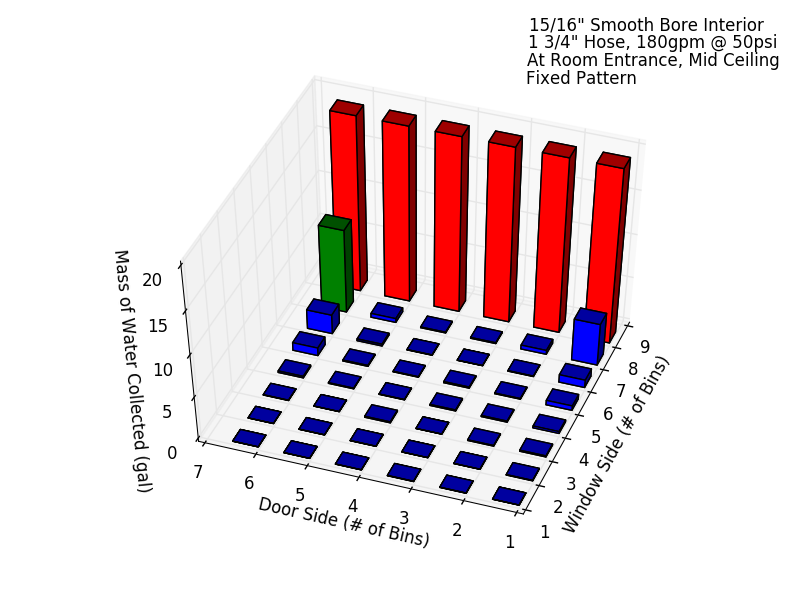
\includegraphics[width=3.2in]{../ADD_Analysis/Figures/15-12-09_144839_Datafile_15_16in_Smooth_Bore_Interior.png}
\caption{Figures showing distribution differences in varying nozzle types during an interior attack with a fixed pattern.}
\label{fig:Interior_Varying_Nozzle_Types_Fixed_Pattern}
\end{figure}

\clearpage

% Interior (at room entrance, O pattern, set flow/pressure)
% 	SS (150 @ 50), Fog (150 @ 50), 15/16 SB (180 @ 50)
% 	15-12-09_122551_Datafile, 15-12-09_123636_Datafile, 15-12-09_145534_Datafile

\begin{figure}[ht]
\begin{tabular*}{\textwidth}{lr}
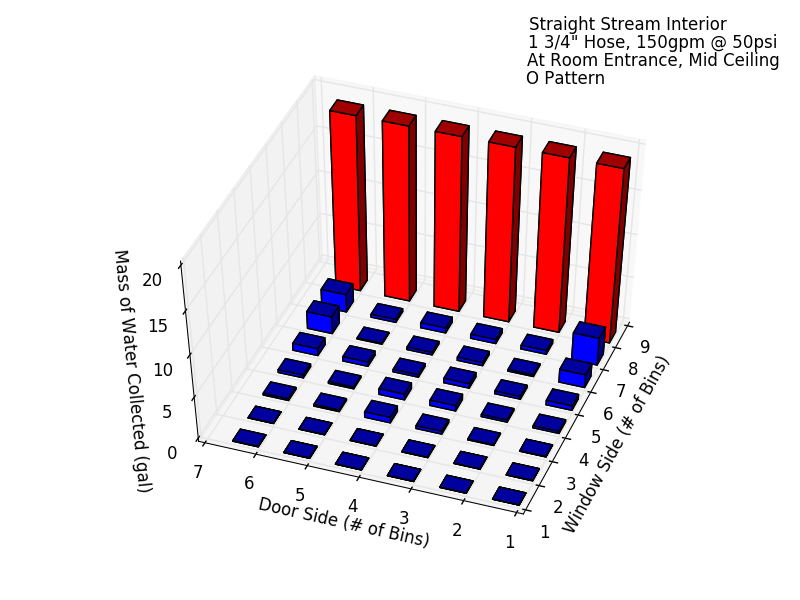
\includegraphics[width=3.2in]{../ADD_Analysis/Figures/15-12-09_122551_Datafile_Straight_Stream_Interior.png} &
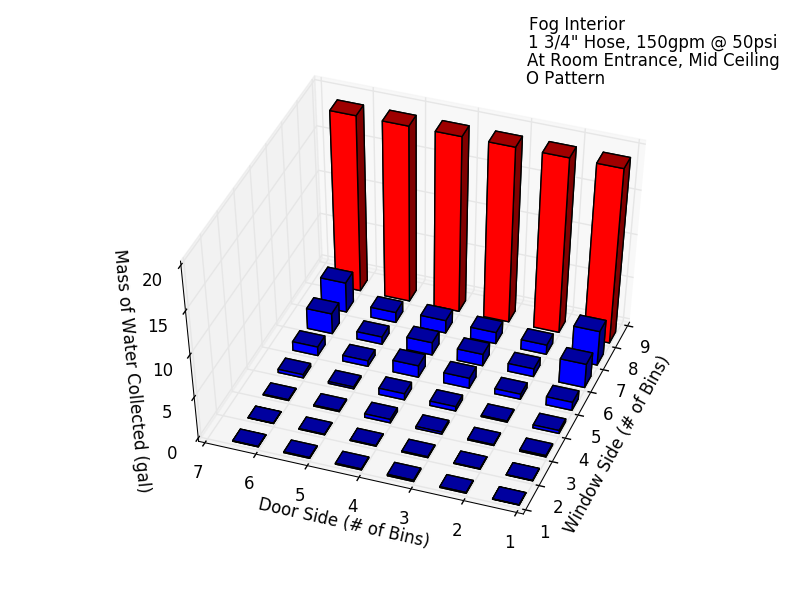
\includegraphics[width=3.2in]{../ADD_Analysis/Figures/15-12-09_123636_Datafile_Fog_Interior.png} \\
\end{tabular*}
\centering
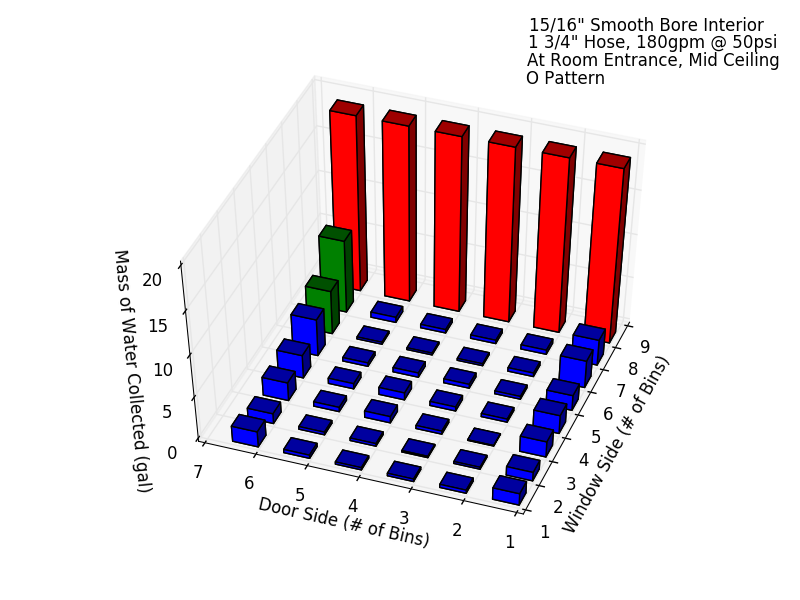
\includegraphics[width=3.2in]{../ADD_Analysis/Figures/15-12-09_145534_Datafile_15_16in_Smooth_Bore_Interior.png}
\caption{Figures showing distribution differences in varying nozzle types during an interior attack with an `O' pattern.}
\label{fig:Interior_Varying_Nozzle_Types_O_Pattern}
\end{figure}

\clearpage

% --------------------------------------------------------------------------------
% Exterior, First Floor/Second Floor
% --------------------------------------------------------------------------------

% % Exterior (first floor, fixed, set flow/pressure)
% % 	SS (150 @ 100), Fog (150 @ 100), 15/16 SB (180 @ 50)
% % 	15-12-08_113237_Datafile, 15-12-08_121806_Datafile, 15-12-08_101028_Datafile

% Exterior (second floor, fixed, set flow/pressure)
% 	SS (150 @ 100), Fog (150 @ 100), 15/16 SB (180 @ 50)
% 	15-12-07_145156_Datafile, 15-12-07_155751_Datafile, 15-12-07_111118_Datafile

\begin{figure}[ht]
\begin{tabular*}{\textwidth}{lr}
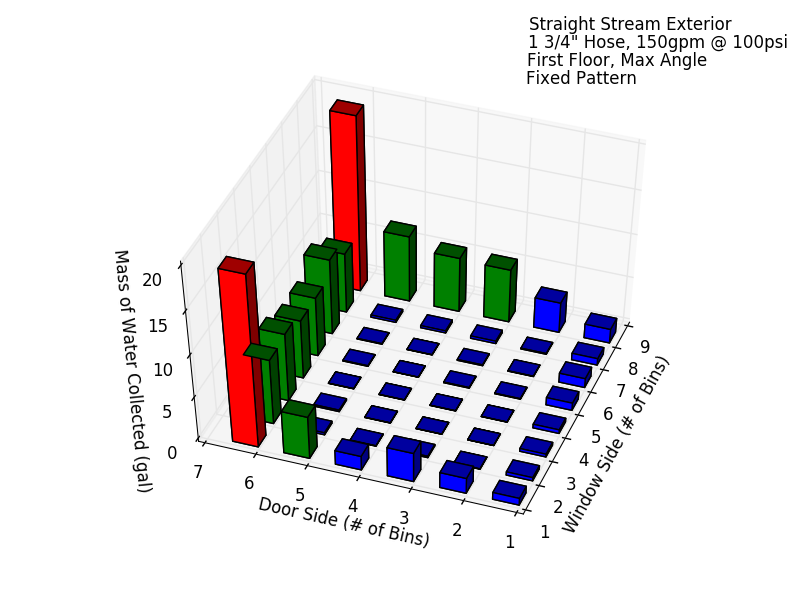
\includegraphics[width=3.2in]{../ADD_Analysis/Figures/15-12-08_113237_Datafile_Straight_Stream_Exterior.png} &
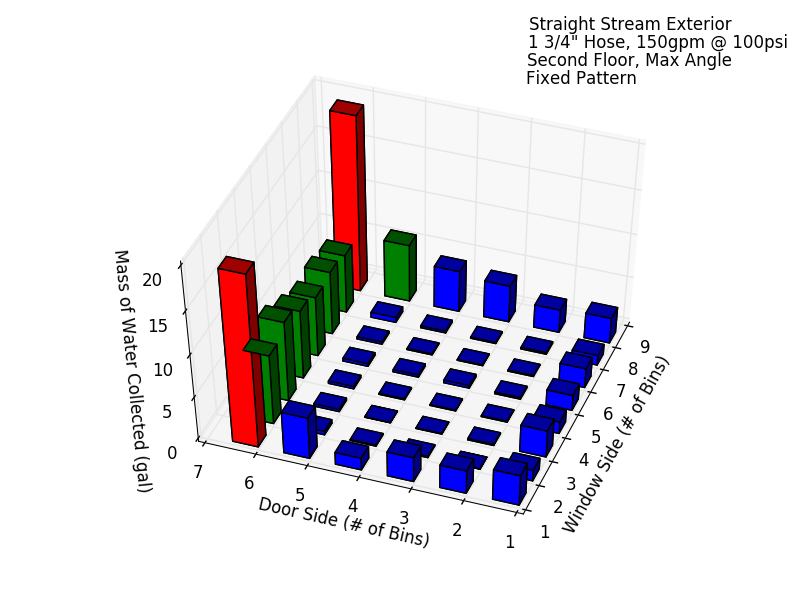
\includegraphics[width=3.2in]{../ADD_Analysis/Figures/15-12-07_145156_Datafile_Straight_Stream_Exterior.png} \\
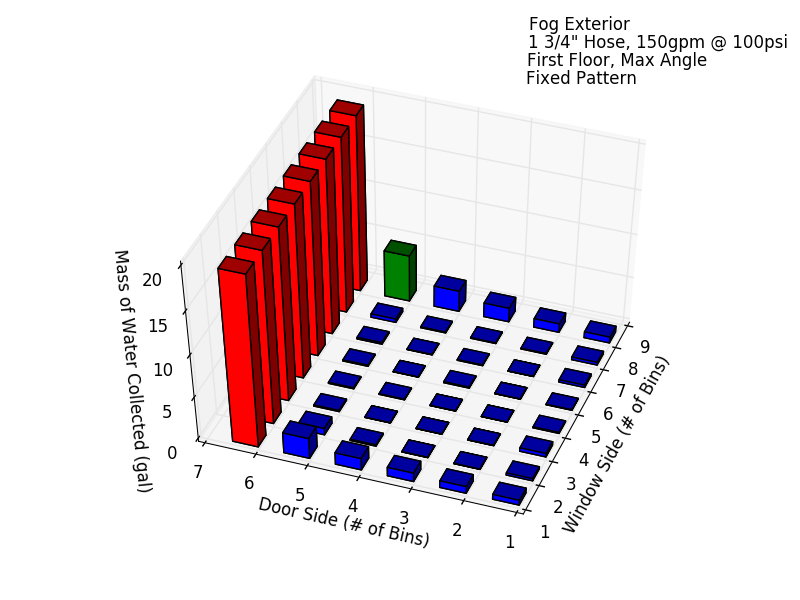
\includegraphics[width=3.2in]{../ADD_Analysis/Figures/15-12-08_121806_Datafile_Fog_Exterior.png} &
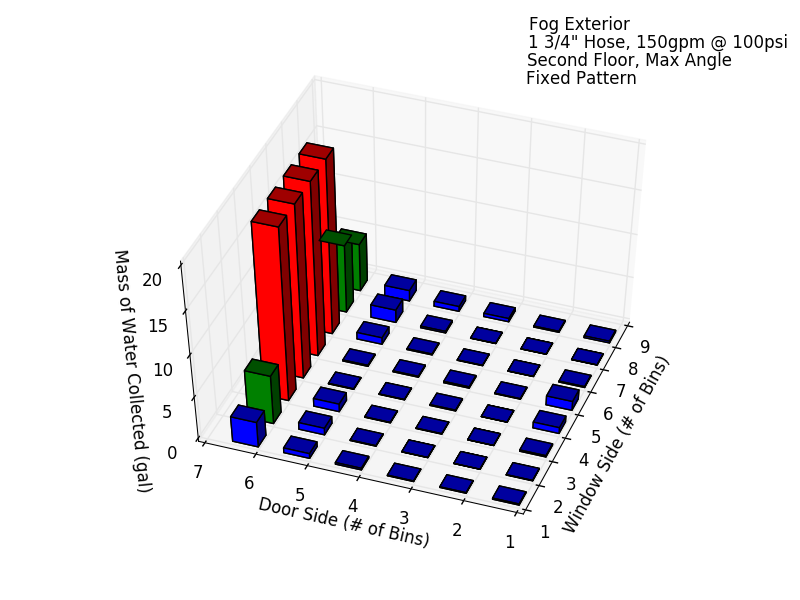
\includegraphics[width=3.2in]{../ADD_Analysis/Figures/15-12-07_155751_Datafile_Fog_Exterior.png} \\
\includegraphics[width=3.2in]{../ADD_Analysis/Figures/15-12-08_101028_Datafile_15_16in_Smooth_Bore_Exterior.png} & 
\includegraphics[width=3.2in]{../ADD_Analysis/Figures/15-12-07_111118_Datafile_15_16in_Smooth_Bore_Exterior.png} \\
\end{tabular*}
\centering
\caption{Figures showing distribution differences in varying nozzle types during an exterior attack with a fixed pattern.}
\label{fig:Exterior_Varying_Nozzle_Types_Fixed_Pattern}
\end{figure}

\clearpage

% Exterior (first floor, Sweeping pattern, set flow/pressure)
% 	SS (150 @ 50), 15/16 SB (180 @ 50)
% 	15-12-08_113716_Datafile, 15-12-08_101825_Datafile

% Exterior (second floor, Sweeping pattern, set flow/pressure)
% 	SS (150 @ 50), 15/16 SB (180 @ 50)
% 	15-12-07_121014_Datafile, 15-12-07_145842_Datafile

\begin{figure}[ht]
\begin{tabular*}{\textwidth}{lr}
\includegraphics[width=3.2in]{../ADD_Analysis/Figures/15-12-08_113716_Datafile_Straight_Stream_Exterior.png} &
\includegraphics[width=3.2in]{../ADD_Analysis/Figures/15-12-07_145842_Datafile_Straight_Stream_Exterior.png} \\
\includegraphics[width=3.2in]{../ADD_Analysis/Figures/15-12-08_101825_Datafile_15_16in_Smooth_Bore_Exterior.png} &
\includegraphics[width=3.2in]{../ADD_Analysis/Figures/15-12-07_121014_Datafile_15_16in_Smooth_Bore_Exterior.png} \\
\end{tabular*}
\caption{Figures showing distribution differences in varying nozzle types during an exterior attack with a sweeping pattern.}
\label{fig:Exterior_Varying_Nozzle_Types_Sweeping_Pattern}
\end{figure}

\clearpage

\paragraph{Water distrubtion is dependent on stream direction within a compartment (max angle, mid ceiling, min angle).} \mbox{}

% ------------------------------------------------------------------------------------
% Interior
% ------------------------------------------------------------------------------------

% Interior (at room entrance, fixed pattern, set flow/pressure: 180 @ 50)
% 	15/16 SB at wall, 15/16 SB mid-ceiling, 15/16 SB max angle
% 	15-12-09_142948_Datafile, 15-12-09_144839_Datafile, 15-12-09_145932_Datafile

\begin{figure}[ht]
\begin{tabular*}{\textwidth}{lr}
\includegraphics[width=3.2in]{../ADD_Analysis/Figures/15-12-09_142948_Datafile_15_16in_Smooth_Bore_Interior.png} &
\includegraphics[width=3.2in]{../ADD_Analysis/Figures/15-12-09_144839_Datafile_15_16in_Smooth_Bore_Interior.png} \\
\end{tabular*}
\centering
\includegraphics[width=3.2in]{../ADD_Analysis/Figures/15-12-09_145932_Datafile_15_16in_Smooth_Bore_Interior.png}
\caption{Figures showing distribution differences in varying nozzle directions during smooth bore attack with a fixed pattern.}
\label{fig:Interior_Varying_Nozzle_Direction_SB_Fixed_Pattern}
\end{figure}

\clearpage

% Interior (at room entrance, O pattern, set flow/pressure: 180 @ 50)
% 	15/16 SB at wall, 15/16 SB mid-ceiling, 15/16 SB max angle
% 	15-12-09_144524_Datafile, 15-12-09_145534_Datafile, 15-12-09_150300_Datafile

\begin{figure}[ht]
\begin{tabular*}{\textwidth}{lr}
\includegraphics[width=3.2in]{../ADD_Analysis/Figures/15-12-09_144524_Datafile_15_16in_Smooth_Bore_Interior.png} &
\includegraphics[width=3.2in]{../ADD_Analysis/Figures/15-12-09_145534_Datafile_15_16in_Smooth_Bore_Interior.png} \\
\end{tabular*}
\centering
\includegraphics[width=3.2in]{../ADD_Analysis/Figures/15-12-09_150300_Datafile_15_16in_Smooth_Bore_Interior.png}
\caption{Figures showing distribution differences in varying nozzle directions during smooth bore attack with an `O' pattern.}
\label{fig:Interior_Varying_Nozzle_Direction_SB_O_Pattern}
\end{figure}

\clearpage

% Interior (at room entrance, fixed pattern, set flow/pressure: 150 @ 100)
% 	SS at wall, SS mid-ceiling, SS max angle
% 	15-12-09_151401_Datafile, 15-12-09_112850_Datafile, 15-12-09_152435_Datafile

\begin{figure}[ht]
\begin{tabular*}{\textwidth}{lr}
\includegraphics[width=3.2in]{../ADD_Analysis/Figures/15-12-09_151401_Datafile_Straight_Stream_Interior.png} &
\includegraphics[width=3.2in]{../ADD_Analysis/Figures/15-12-09_112850_Datafile_Straight_Stream_Interior.png} \\
\end{tabular*}
\centering
\includegraphics[width=3.2in]{../ADD_Analysis/Figures/15-12-09_152435_Datafile_Straight_Stream_Interior.png}
\caption{Figures showing distribution differences in varying nozzle directions during a straight stream attack with a fixed pattern.}
\label{fig:Interior_Varying_Nozzle_Direction_SS_Fixed_Pattern}
\end{figure}

\clearpage

% Interior (at room entrance, O pattern, set flow/pressure: 150 @ 100)
% 	SS at wall, SS mid-ceiling, SS max angle
% 	15-12-09_151823_Datafile, 15-12-09_113335_Datafile, 15-12-09_153038_Datafile

\begin{figure}[ht]
\begin{tabular*}{\textwidth}{lr}
\includegraphics[width=3.2in]{../ADD_Analysis/Figures/15-12-09_151823_Datafile_Straight_Stream_Interior.png} &
\includegraphics[width=3.2in]{../ADD_Analysis/Figures/15-12-09_113335_Datafile_Straight_Stream_Interior.png} \\
\end{tabular*}
\centering
\includegraphics[width=3.2in]{../ADD_Analysis/Figures/15-12-09_153038_Datafile_Straight_Stream_Interior.png}
\caption{Figures showing distribution differences in varying nozzle directions during a straight stream attack with an `O' pattern.}
\label{fig:Interior_Varying_Nozzle_Direction_SS_O_Pattern}
\end{figure}

\clearpage

% -----------------------------------------------------------------------------
% Exterior, First Floor/Second Floor
% -----------------------------------------------------------------------------

\begin{figure}[ht]
\begin{tabular*}{\textwidth}{lr}
\includegraphics[width=3.2in]{../ADD_Analysis/Figures/15-12-08_113237_Datafile_Straight_Stream_Exterior.png} &
\includegraphics[width=3.2in]{../ADD_Analysis/Figures/15-12-08_114905_Datafile_Straight_Stream_Exterior.png} \\
\includegraphics[width=3.2in]{../ADD_Analysis/Figures/15-12-08_120311_Datafile_Straight_Stream_Exterior.png} &
\includegraphics[width=3.2in]{../ADD_Analysis/Figures/15-12-08_121011_Datafile_Straight_Stream_Exterior.png} \\
\end{tabular*}
\centering
\includegraphics[width=3.2in]{../ADD_Analysis/Figures/15-12-08_121425_Datafile_Straight_Stream_Exterior.png} \\
\caption{Figures showing distribution differences in varying nozzle directions during an exterior first floor attack with a SS fixed pattern.}
\label{fig:Exterior_First_Floor_Varying_Nozzle_Directions_SS_Fixed_Pattern}
\end{figure}

\clearpage

\begin{figure}[ht]
\begin{tabular*}{\textwidth}{lr}
\includegraphics[width=3.2in]{../ADD_Analysis/Figures/15-12-07_145156_Datafile_Straight_Stream_Exterior.png} &
\includegraphics[width=3.2in]{../ADD_Analysis/Figures/15-12-07_151001_Datafile_Straight_Stream_Exterior.png} \\
\includegraphics[width=3.2in]{../ADD_Analysis/Figures/15-12-07_151630_Datafile_Straight_Stream_Exterior.png} &
\includegraphics[width=3.2in]{../ADD_Analysis/Figures/15-12-07_152028_Datafile_Straight_Stream_Exterior.png} \\
\end{tabular*}
\centering
\includegraphics[width=3.2in]{../ADD_Analysis/Figures/15-12-07_155226_Datafile_Straight_Stream_Exterior.png} \\
\caption{Figures showing distribution differences in varying nozzle directions during an exterior second floor attack with a SS fixed pattern.}
\label{fig:Exterior_Second_Floor_Varying_Nozzle_Directions_SS_Fixed_Pattern}
\end{figure}

\clearpage

\begin{figure}[ht]
\begin{tabular*}{\textwidth}{lr}
\includegraphics[width=3.2in]{../ADD_Analysis/Figures/15-12-08_101028_Datafile_15_16in_Smooth_Bore_Exterior.png} &
\includegraphics[width=3.2in]{../ADD_Analysis/Figures/15-12-08_102802_Datafile_15_16in_Smooth_Bore_Exterior.png} \\
\includegraphics[width=3.2in]{../ADD_Analysis/Figures/15-12-08_103414_Datafile_15_16in_Smooth_Bore_Exterior.png} &
\includegraphics[width=3.2in]{../ADD_Analysis/Figures/15-12-08_104150_Datafile_15_16in_Smooth_Bore_Exterior.png} \\
\end{tabular*}
\centering
\includegraphics[width=3.2in]{../ADD_Analysis/Figures/15-12-08_104620_Datafile_15_16in_Smooth_Bore_Exterior.png} \\
\caption{Figures showing distribution differences in varying nozzle directions during an exterior first floor attack with a SB fixed pattern.}
\label{fig:Exterior_First_Floor_Varying_Nozzle_Directions_SB_Fixed_Pattern}
\end{figure}

\clearpage

\begin{figure}[ht]
\begin{tabular*}{\textwidth}{lr}
\includegraphics[width=3.2in]{../ADD_Analysis/Figures/15-12-07_111118_Datafile_15_16in_Smooth_Bore_Exterior.png} &
\includegraphics[width=3.2in]{../ADD_Analysis/Figures/15-12-07_122135_Datafile_15_16in_Smooth_Bore_Exterior.png} \\
\includegraphics[width=3.2in]{../ADD_Analysis/Figures/15-12-07_140034_Datafile_15_16in_Smooth_Bore_Exterior.png} &
\includegraphics[width=3.2in]{../ADD_Analysis/Figures/15-12-07_141333_Datafile_15_16in_Smooth_Bore_Exterior.png} \\
\end{tabular*}
\caption{Figures showing distribution differences in varying nozzle directions during an exterior second floor attack with a SB fixed pattern.}
\label{fig:Exterior_Second_Floor_Varying_Nozzle_Directions_SB_Fixed_Pattern}
\end{figure}

\clearpage

\paragraph{Varying nozzle pressure and flow can affect the amount of water applied to a given area while the distribution remains somewhat constant.} \mbox{}

% ------------------------------------------------------------------------------------
% Interior
% ------------------------------------------------------------------------------------

% Interior (at room entrance, fixed, SS, mid-ceiling)
% 	150 @ 100, 150 @ 75, 150 @ 50
% 	15-12-09_112850_Datafile, 15-12-09_115707_Datafile, 15-12-09_121955_Datafile

\begin{figure}[ht]
\begin{tabular*}{\textwidth}{lr}
\includegraphics[width=3.2in]{../ADD_Analysis/Figures/15-12-09_112850_Datafile_Straight_Stream_Interior.png} &
\includegraphics[width=3.2in]{../ADD_Analysis/Figures/15-12-09_115707_Datafile_Straight_Stream_Interior.png} \\
\end{tabular*}
\centering
\includegraphics[width=3.2in]{../ADD_Analysis/Figures/15-12-09_121955_Datafile_Straight_Stream_Interior.png}
\caption{Figures showing distribution differences in varying nozzle pressures during a straight stream attack with a fixed pattern.}
\label{fig:Interior_Varying_Nozzle_Pressure_SS_Fixed_Pattern}
\end{figure}

\clearpage

% Interior (at room entrance, fixed, fog, mid-ceiling)
% 	150 @ 100, 150 @ 75, 150 @ 50
% 	15-12-09_113802_Datafile, 15-12-09_120821_Datafile, 15-12-09_123142_Datafile

\begin{figure}[ht]
\begin{tabular*}{\textwidth}{lr}
\includegraphics[width=3.2in]{../ADD_Analysis/Figures/15-12-09_113802_Datafile_Fog_Interior.png} &
\includegraphics[width=3.2in]{../ADD_Analysis/Figures/15-12-09_120821_Datafile_Fog_Interior.png} \\
\end{tabular*}
\centering
\includegraphics[width=3.2in]{../ADD_Analysis/Figures/15-12-09_123142_Datafile_Fog_Interior.png}
\caption{Figures showing distribution differences in varying nozzle pressures during a fog attack with a fixed pattern.}
\label{fig:Interior_Varying_Nozzle_Pressure_Fog_Fixed_Pattern}
\end{figure}

\clearpage

% ------------------------------------------------------------------------------------
% Exterior First Floor/Second Floor
% ------------------------------------------------------------------------------------

\begin{figure}[ht]
\begin{tabular*}{\textwidth}{lr}
\includegraphics[width=3.2in]{../ADD_Analysis/Figures/15-12-08_160630_Datafile_Straight_Stream_Exterior.png} &
\includegraphics[width=3.2in]{../ADD_Analysis/Figures/15-12-08_161540_Datafile_Straight_Stream_Exterior.png} \\
\includegraphics[width=3.2in]{../ADD_Analysis/Figures/15-12-08_162126_Datafile_Straight_Stream_Exterior.png} &
\includegraphics[width=3.2in]{../ADD_Analysis/Figures/15-12-08_162547_Datafile_Straight_Stream_Exterior.png} \\
\end{tabular*}
\caption{Figures showing distribution differences in varying nozzle pressures during an exterior first floor straight stream attack with a fixed pattern.}
\label{fig:Exterior_First_Floor_Varying_Nozzle_Pressure_SS_Fixed_Pattern}
\end{figure}

\clearpage

\begin{figure}[ht]
\begin{tabular*}{\textwidth}{lr}
\includegraphics[width=3.2in]{../ADD_Analysis/Figures/15-12-08_153737_Datafile_15_16in_Smooth_Bore_Exterior.png} &
\includegraphics[width=3.2in]{../ADD_Analysis/Figures/15-12-08_154306_Datafile_15_16in_Smooth_Bore_Exterior.png} \\
\includegraphics[width=3.2in]{../ADD_Analysis/Figures/15-12-08_154812_Datafile_15_16in_Smooth_Bore_Exterior.png} &
\includegraphics[width=3.2in]{../ADD_Analysis/Figures/15-12-08_155710_Datafile_15_16in_Smooth_Bore_Exterior.png} \\
\end{tabular*}
\caption{Figures showing distribution differences in varying nozzle pressures during an exterior first floor smooth bore attack with a fixed pattern.}
\label{fig:Exterior_First_Floor_Varying_Nozzle_Pressure_SB_Fixed_Pattern}
\end{figure}

\clearpage

\begin{figure}[ht]
\begin{tabular*}{\textwidth}{lr}
\includegraphics[width=3.2in]{../ADD_Analysis/Figures/15-12-07_111118_Datafile_15_16in_Smooth_Bore_Exterior.png} &
\includegraphics[width=3.2in]{../ADD_Analysis/Figures/15-12-07_143141_Datafile_7_8in_Smooth_Bore_Exterior.png} \\
\end{tabular*}
\centering
\includegraphics[width=3.2in]{../ADD_Analysis/Figures/15-12-07_143828_Datafile_1in_Smooth_Bore_Exterior.png}
\caption{Figures showing distribution differences in varying nozzle flows by increasing the tip size during an exterior second floor smooth bore attack with a fixed pattern.}
\label{fig:Exterior_Second_Floor_Varying_Nozzle_Pressure_SB_Fixed_Pattern}
\end{figure}

\clearpage

\paragraph{Applying water from the exterior or from a distance via the interior will adequately coat the surfaces of a compartment (walls and ceiling) while applying little water to the center of the room.} \mbox{}

% Interior (at room entrance, fixed, SB, max angle) - 15-12-09_145932_Datafile
% 		 (at room entrance, fixed, fog, mid-ceiling) - 15-12-09_113802_Datafile

\begin{figure}[ht]
\begin{tabular*}{\textwidth}{lr}
\includegraphics[width=3.2in]{../ADD_Analysis/Figures/15-12-09_145932_Datafile_15_16in_Smooth_Bore_Interior.png} &
\includegraphics[width=3.2in]{../ADD_Analysis/Figures/15-12-09_113802_Datafile_Fog_Interior.png} \\
\end{tabular*}
\caption{Figures showing lack of adequate coverage to the center of the room from an interior attack.}
\label{fig:Lack_of_Center_Coverage_Interior}
\end{figure}

% ----------------------------------------------------------------------------

\begin{figure}[ht]
\begin{tabular*}{\textwidth}{lr}
\includegraphics[width=3.2in]{../ADD_Analysis/Figures/15-12-08_101028_Datafile_15_16in_Smooth_Bore_Exterior.png} &
\includegraphics[width=3.2in]{../ADD_Analysis/Figures/15-12-08_121806_Datafile_Fog_Exterior.png} \\
\end{tabular*}
\caption{Figures showing lack of adequate coverage to the center of the room from an exterior attack.}
\label{fig:Lack_of_Center_Coverage_Exterior}
\end{figure}

From both the fire tests as well as the non-fire tests, it is evident that little to no water makes it into the center of the room given an attack featuring the nozzle directed at either the ceiling or the side walls of the compartment.

\vspace*{\baselineskip}

\clearpage

\section{Future Research Needs}

Part I of the Fire Attack Study was intended to provide preliminary results and insight into the amount of air entrained by hose streams using differing nozzles and configurations in addition to determining where water is distributed within compartments. These tests have built upon the work conducted by Knapp et. all of the Rockland County, NY Fire Training Academy who conducted early experiments to attempt to quantify the amount of air entrained by suppression operations. Because the testing scope was limied to certain geometries for both air entrainment and water distribution, a future study analyzing different sized structures (including a varying ceiling height and design) in addition to differing compartmentation versus open concepts would be beneficial to further the understanding.

% ****** REMOVE COMMRENTS IN THIS BLOCK TO ADD GLOSSARY SEE IN HEADER FOR OTHER BLOCK TO REMOVE ***********
% \clearpage

% \glsaddall
% \printglossary[nonumberlist]
% \newpage

\printbibliography

\clearpage

\begin{appendices}

\section{Experimental Results} \label{App:Results}
\renewcommand{\thesubsection}{\Alph{section}}
\counterwithin{figure}{subsection}

\appendix


\chapter{Air Entrainment Figures}
\label{app:Air_Entrainment_Figures}

Section currently commented out.

\chapter{Water Distribution Figures}
\label{app:Water_Distribution_Figures}

Section currently commented out.

% \begin{figure}[ht]
% \begin{tabular*}{\textwidth}{lr}
% \includegraphics[width=3.2in]{../ADD_Analysis/Figures/15-04-13_103117_Datafile_Fog_Interior.png} &
% \includegraphics[width=3.2in]{../ADD_Analysis/Figures/15-12-07_111118_Datafile_15_16in_Smooth_Bore_Exterior.png} \\
% \includegraphics[width=3.2in]{../ADD_Analysis/Figures/15-12-07_121014_Datafile_15_16in_Smooth_Bore_Exterior.png} &
% \includegraphics[width=3.2in]{../ADD_Analysis/Figures/15-12-07_122135_Datafile_15_16in_Smooth_Bore_Exterior.png}
% \end{tabular*}
% \caption{Spray density figures for burn building tests 1) Water Straight Stream Back (upper left), 2) Water Straight Stream Back (upper right), 3) Water Straight Stream Mid (lower left), and 4) Water Straight Stream Mid (lower right)}
% \label{fig:15/16_Smooth_Bore_Exterior}
% \end{figure}

% \clearpage

% \begin{figure}[ht]
% \begin{tabular*}{\textwidth}{lr}
% \includegraphics[width=3.2in]{../Figures/Bars/BB5} &
% \includegraphics[width=3.2in]{../Figures/Bars/BB6} \\
% \includegraphics[width=3.2in]{../Figures/Bars/BB7} &
% \includegraphics[width=3.2in]{../Figures/Bars/BB8}
% \end{tabular*}
% \caption{Spray density figures for burn building tests 5) Water Straight Stream Mid (upper left), 6) Water Fog Mid (upper right), 7) Water Fog Mid (lower left), and 8) Water Fog Back (lower right)}
% \label{fig:bb_5_8}
% \end{figure}

% \clearpage

% \begin{figure}[ht]
% \begin{tabular*}{\textwidth}{lr}
% \includegraphics[width=3.2in]{../Figures/Bars/BB9} &
% \includegraphics[width=3.2in]{../Figures/Bars/BB10} \\
% \includegraphics[width=3.2in]{../Figures/Bars/BB11} &
% \includegraphics[width=3.2in]{../Figures/Bars/BB12}
% \end{tabular*}
% \caption{Spray density figures for burn building tests 9) Water Fog Back (upper left), 10) Water Solid Stream Back (upper right), 11) Water Solid Stream Back (lower left), and 12) CAF Solid Stream Back (lower right)}
% \label{fig:bb_9_12}
% \end{figure}

% \clearpage

% \begin{figure}[ht]
% \begin{tabular*}{\textwidth}{lr}
% \includegraphics[width=3.2in]{../Figures/Bars/BB13} &
% \includegraphics[width=3.2in]{../Figures/Bars/BB14} \\
% \includegraphics[width=3.2in]{../Figures/Bars/BB15} &
% \includegraphics[width=3.2in]{../Figures/Bars/BB16}
% \end{tabular*}
% \caption{Spray density figures for burn building tests 13) CAF Solid Stream Mid (upper left), 14) CAF Solid Stream Back (upper right), 15) CAF Solid Stream Mid (lower left), and 16) CAF Fog Mid (lower right)}
% \label{fig:bb_13_16}
% \end{figure}

% \clearpage

% \begin{figure}[ht]
% \begin{tabular*}{\textwidth}{lr}
% \includegraphics[width=3.2in]{../Figures/Bars/BB17} &
% \includegraphics[width=3.2in]{../Figures/Bars/BB18} \\
% \includegraphics[width=3.2in]{../Figures/Bars/BB19} &
% \includegraphics[width=3.2in]{../Figures/Bars/BB20}
% \end{tabular*}
% \caption{Spray density figures for burn building tests 17) CAF Straight Stream Mid (upper left), 18) CAF Straight Stream Mid (upper right), 19) CAF Fog Back (lower left), and 20) CAF Fog Back (lower right)}
% \label{fig:bb_19_21}
% \end{figure}

% \clearpage

% \begin{figure}[ht]
% \centering
% \includegraphics[width=3.2in]{../Figures/Bars/BB21}
% \caption{Spray density figures for burn building test 21) CAF Straight Stream Back}
% \label{fig:bb_21}
% \end{figure}

% \clearpage

% \section{Spray density figures for experimental structure tests}

% \begin{figure}[ht]
% \begin{tabular*}{\textwidth}{lr}
% \includegraphics[width=3.2in]{../Figures/Bars/ES_1} &
% \includegraphics[width=3.2in]{../Figures/Bars/ES_2} \\
% \includegraphics[width=3.2in]{../Figures/Bars/ES_3} &
% \includegraphics[width=3.2in]{../Figures/Bars/ES_4}
% \end{tabular*}
% \caption{Spray density figures for experimental structure tests 1) Water Straight Stream FR (upper left), 2) Water Straight Stream FR (upper right), 3) Water Straight Stream FR (lower left), and 4) Water Straight Stream FR (lower right)}
% \label{fig:es_1_4}
% \end{figure}

% \clearpage

% \begin{figure}[ht]
% \begin{tabular*}{\textwidth}{lr}
% \includegraphics[width=3.2in]{../Figures/Bars/ES_5} &
% \includegraphics[width=3.2in]{../Figures/Bars/ES_6} \\
% \includegraphics[width=3.2in]{../Figures/Bars/ES_7} &
% \includegraphics[width=3.2in]{../Figures/Bars/ES_72}
% \end{tabular*}
% \caption{Spray density figures for experimental structure tests 5) Water Fog FR (upper left), 6) Water Fog FR (upper right), 7) Water Solid Stream FR (lower left), and 8) Water Solid Stream H (lower right)}
% \label{fig:es_5_72}
% \end{figure}

% \clearpage

% \begin{figure}[ht]
% \begin{tabular*}{\textwidth}{lr}
% \includegraphics[width=3.2in]{../Figures/Bars/ES_8} &
% \includegraphics[width=3.2in]{../Figures/Bars/ES_9} \\
% \includegraphics[width=3.2in]{../Figures/Bars/ES_10} &
% \includegraphics[width=3.2in]{../Figures/Bars/ES_11}
% \end{tabular*}
% \caption{Spray density figures for experimental structure tests 9) Water Fog H (upper left), 10) Water Fog H (upper right), 11) Water Straight Stream H (lower left), and 12) Water Straight Stream H (lower right)}
% \label{fig:es_8_11}
% \end{figure}

% \clearpage		\large
% \subsection{Experiment 1 Results} \label{App:Exp1Results} 

%\begin{figure}[h!]
%	\centering
%	\includegraphics[height=3.05in]{}
%	\caption{Experiment 1 - Chart Name}
%\end{figure}
%
%
%\begin{figure}[h!]
%	\centering
%	\includegraphics[height=3.05in]{}
%	\caption{Experiment 1 - Chart Name}
%\end{figure}

\clearpage

\end{appendices}

\end{document}

